% Options for packages loaded elsewhere
\PassOptionsToPackage{unicode}{hyperref}
\PassOptionsToPackage{hyphens}{url}
%
\documentclass[
  9pt,
]{extbook}
\usepackage{lmodern}
\usepackage{amsmath}
\usepackage{ifxetex,ifluatex}
\ifnum 0\ifxetex 1\fi\ifluatex 1\fi=0 % if pdftex
  \usepackage[T1]{fontenc}
  \usepackage[utf8]{inputenc}
  \usepackage{textcomp} % provide euro and other symbols
  \usepackage{amssymb}
\else % if luatex or xetex
  \usepackage{unicode-math}
  \defaultfontfeatures{Scale=MatchLowercase}
  \defaultfontfeatures[\rmfamily]{Ligatures=TeX,Scale=1}
\fi
% Use upquote if available, for straight quotes in verbatim environments
\IfFileExists{upquote.sty}{\usepackage{upquote}}{}
\IfFileExists{microtype.sty}{% use microtype if available
  \usepackage[]{microtype}
  \UseMicrotypeSet[protrusion]{basicmath} % disable protrusion for tt fonts
}{}
\makeatletter
\@ifundefined{KOMAClassName}{% if non-KOMA class
  \IfFileExists{parskip.sty}{%
    \usepackage{parskip}
  }{% else
    \setlength{\parindent}{0pt}
    \setlength{\parskip}{6pt plus 2pt minus 1pt}}
}{% if KOMA class
  \KOMAoptions{parskip=half}}
\makeatother
\usepackage{xcolor}
\IfFileExists{xurl.sty}{\usepackage{xurl}}{} % add URL line breaks if available
\IfFileExists{bookmark.sty}{\usepackage{bookmark}}{\usepackage{hyperref}}
\hypersetup{
  pdftitle={The Live Textbook of Physical Chemistry 2},
  pdfauthor={Dr.~Roberto Peverati},
  hidelinks,
  pdfcreator={LaTeX via pandoc}}
\urlstyle{same} % disable monospaced font for URLs
\usepackage{longtable,booktabs}
\usepackage{calc} % for calculating minipage widths
% Correct order of tables after \paragraph or \subparagraph
\usepackage{etoolbox}
\makeatletter
\patchcmd\longtable{\par}{\if@noskipsec\mbox{}\fi\par}{}{}
\makeatother
% Allow footnotes in longtable head/foot
\IfFileExists{footnotehyper.sty}{\usepackage{footnotehyper}}{\usepackage{footnote}}
\makesavenoteenv{longtable}
\usepackage{graphicx}
\makeatletter
\def\maxwidth{\ifdim\Gin@nat@width>\linewidth\linewidth\else\Gin@nat@width\fi}
\def\maxheight{\ifdim\Gin@nat@height>\textheight\textheight\else\Gin@nat@height\fi}
\makeatother
% Scale images if necessary, so that they will not overflow the page
% margins by default, and it is still possible to overwrite the defaults
% using explicit options in \includegraphics[width, height, ...]{}
\setkeys{Gin}{width=\maxwidth,height=\maxheight,keepaspectratio}
% Set default figure placement to htbp
\makeatletter
\def\fps@figure{htbp}
\makeatother
\setlength{\emergencystretch}{3em} % prevent overfull lines
\providecommand{\tightlist}{%
  \setlength{\itemsep}{0pt}\setlength{\parskip}{0pt}}
\setcounter{secnumdepth}{5}
\usepackage{booktabs}
\usepackage{pdfpages}
\usepackage{amsthm}
\usepackage[version=4]{mhchem}
\usepackage{cancel}

%change to a smaller page:
\usepackage[paperwidth=6in, paperheight=9in]{geometry}
% this is to change the size of text: headsep=10pt, textheight=550pt
%\usepackage[textwidth=456pt]{geometry}

%fancyhdr to set custom headers for the book:
\usepackage{fancyhdr}
\pagestyle{fancy}
\fancyhf{}
\fancyhead[LO]{\slshape\nouppercase{\rightmark}}
\fancyhead[RE]{\slshape\nouppercase{\leftmark}}
\fancyhead[RO,LE]{\thepage}
%no page numbers on empty pages
\let\origdoublepage\cleardoublepage
\newcommand{\clearemptydoublepage}{%
  \clearpage
  {\pagestyle{empty}\origdoublepage}%
}
\let\cleardoublepage\clearemptydoublepage


\makeatletter
\def\thm@space@setup{%
  \thm@preskip=8pt plus 2pt minus 4pt
  \thm@postskip=\thm@preskip
}
\makeatother
\let\oldmaketitle\maketitle
\AtBeginDocument{\let\maketitle\relax}
\ifluatex
  \usepackage{selnolig}  % disable illegal ligatures
\fi
\usepackage[]{natbib}
\bibliographystyle{apalike}

\title{The Live Textbook of Physical Chemistry 2}
\author{\href{mailto:rpeverati@fit.edu}{Dr.~Roberto Peverati}}
\date{27 January 2021}

\usepackage{amsthm}
\newtheorem{theorem}{Theorem}[chapter]
\newtheorem{lemma}{Lemma}[chapter]
\newtheorem{corollary}{Corollary}[chapter]
\newtheorem{proposition}{Proposition}[chapter]
\newtheorem{conjecture}{Conjecture}[chapter]
\theoremstyle{definition}
\newtheorem{definition}{Definition}[chapter]
\theoremstyle{definition}
\newtheorem{example}{Example}[chapter]
\theoremstyle{definition}
\newtheorem{exercise}{Exercise}[chapter]
\theoremstyle{remark}
\newtheorem*{remark}{Remark}
\newtheorem*{solution}{Solution}
\begin{document}
\maketitle

%Frontpage for 6x9:
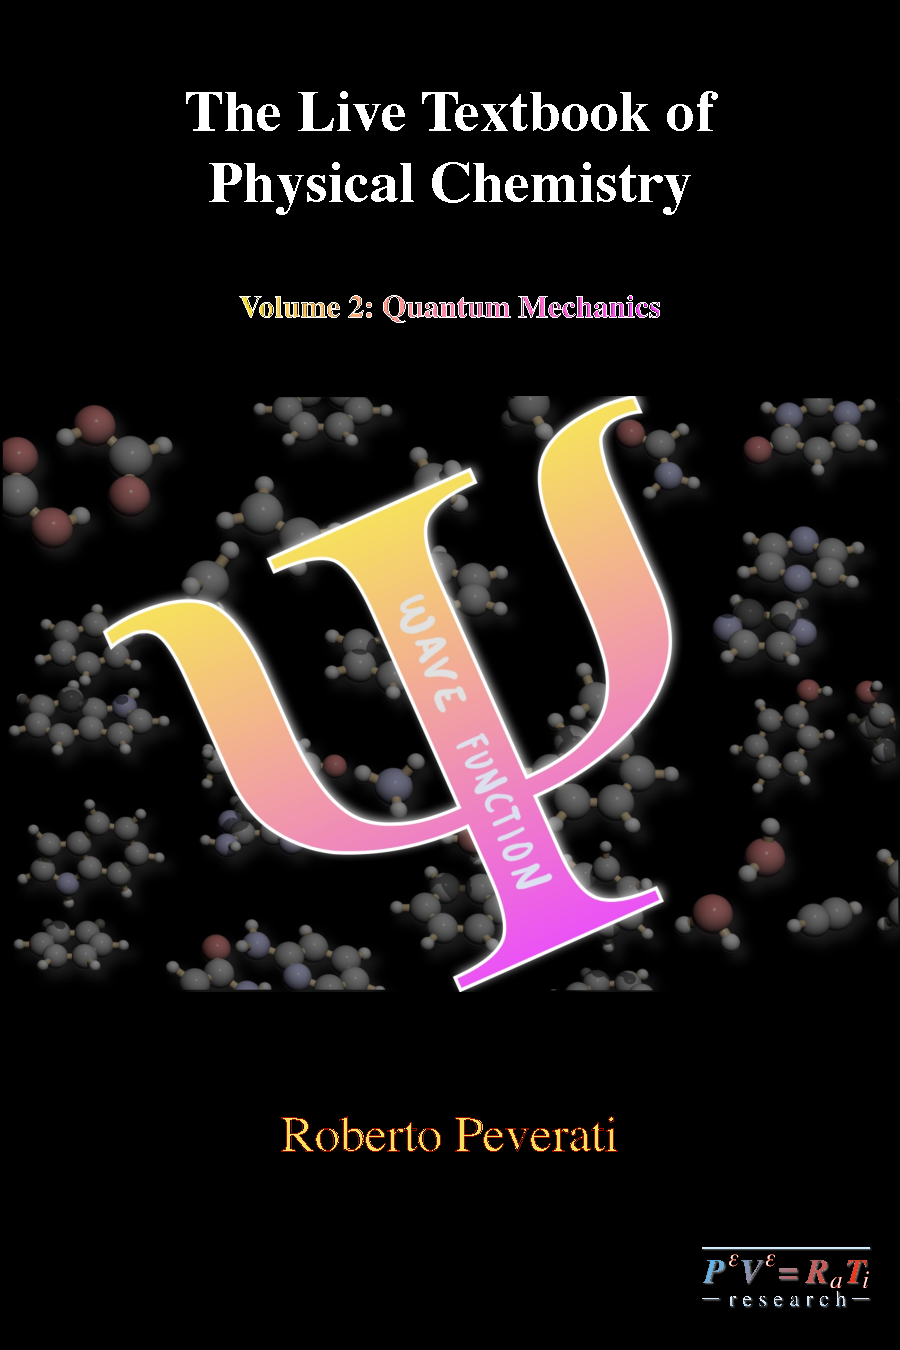
\includepdf[pages={1}, scale=1]{FrontPage_6x9.pdf}
%Frontpage for USLetter:
%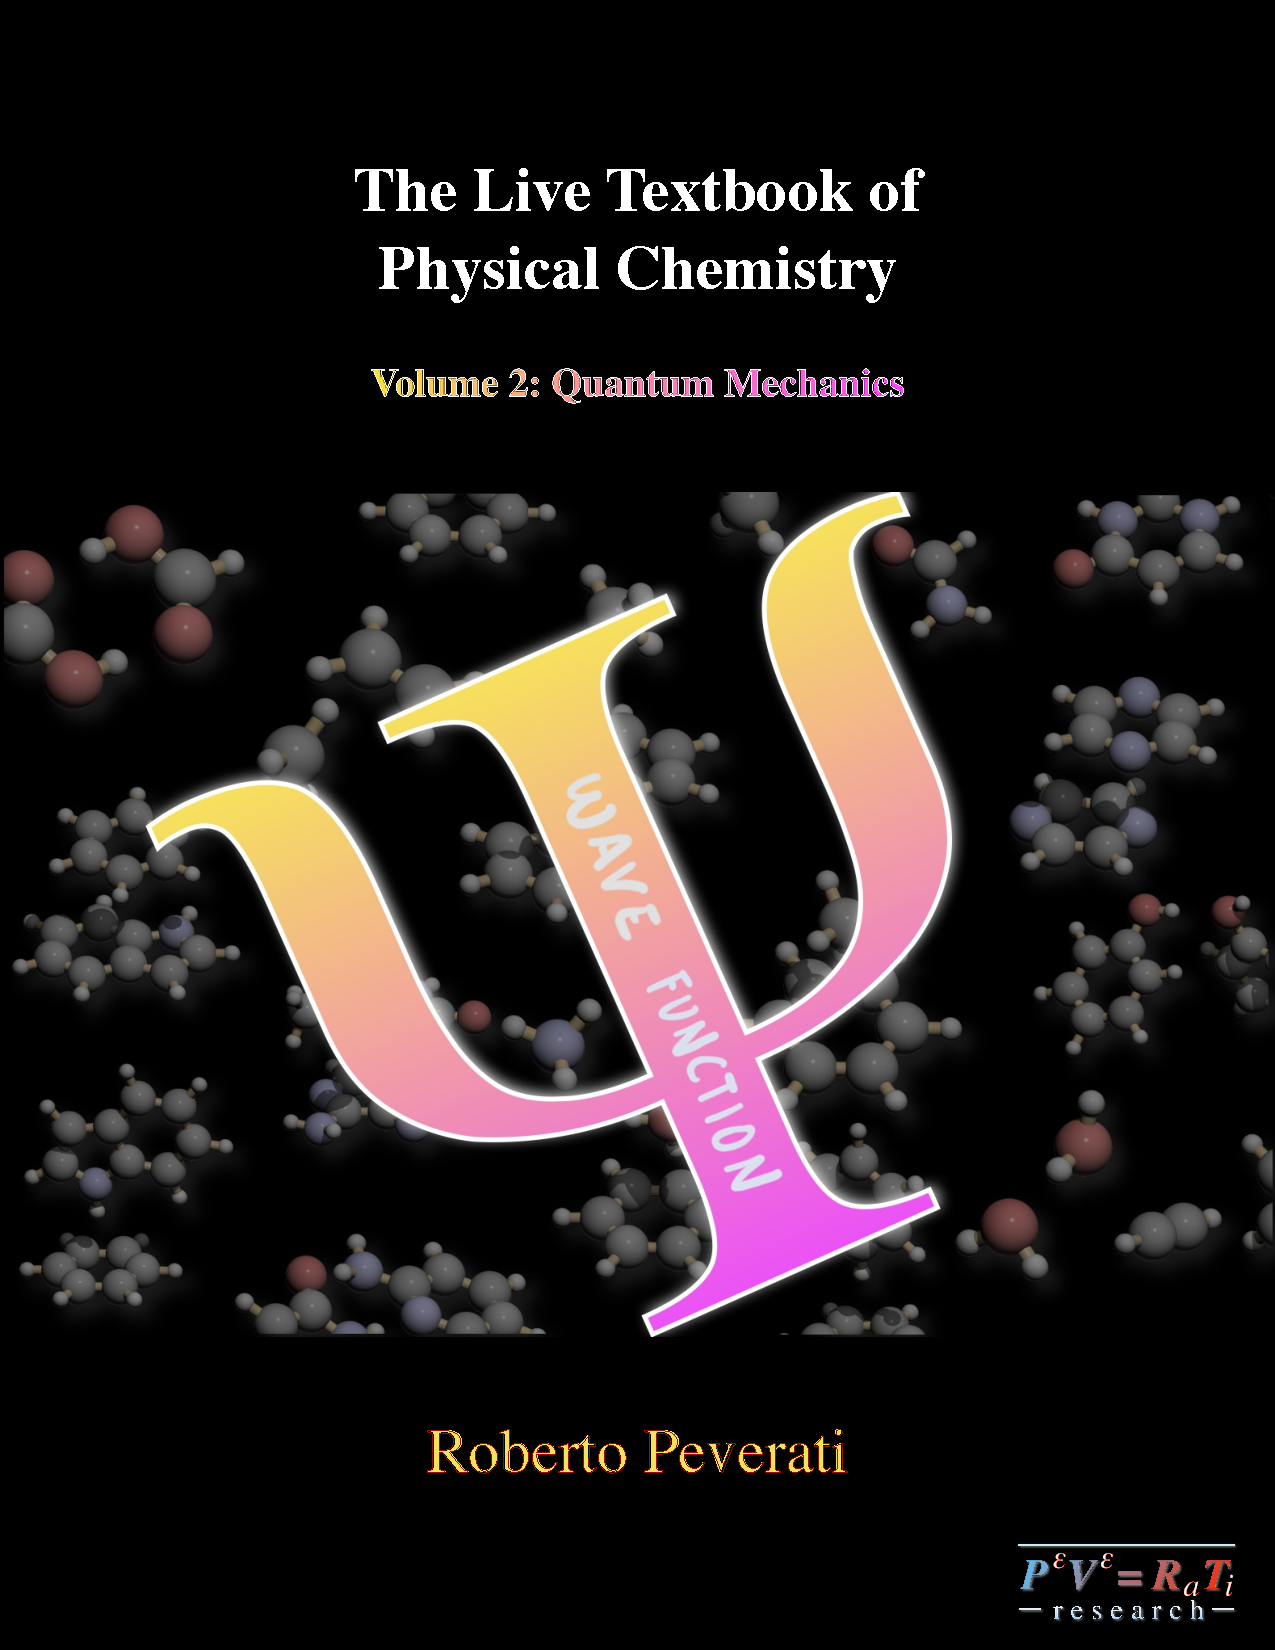
\includepdf[pages={1}, scale=1]{FrontPage.pdf}
\newpage

\let\maketitle\oldmaketitle

% Let's change \thepage so it prints one less than
% the real page number; \pagenumbering{arabic}
% will redefine it to the right meaning afterwards.
\renewcommand\thepage{\romannumeral\numexpr\value{page}-1\relax}


{
\setcounter{tocdepth}{1}
\tableofcontents
}
\renewcommand{\arraystretch}{1.8}

\hypertarget{preface}{%
\chapter*{Preface}\label{preface}}
\addcontentsline{toc}{chapter}{Preface}

\begin{center}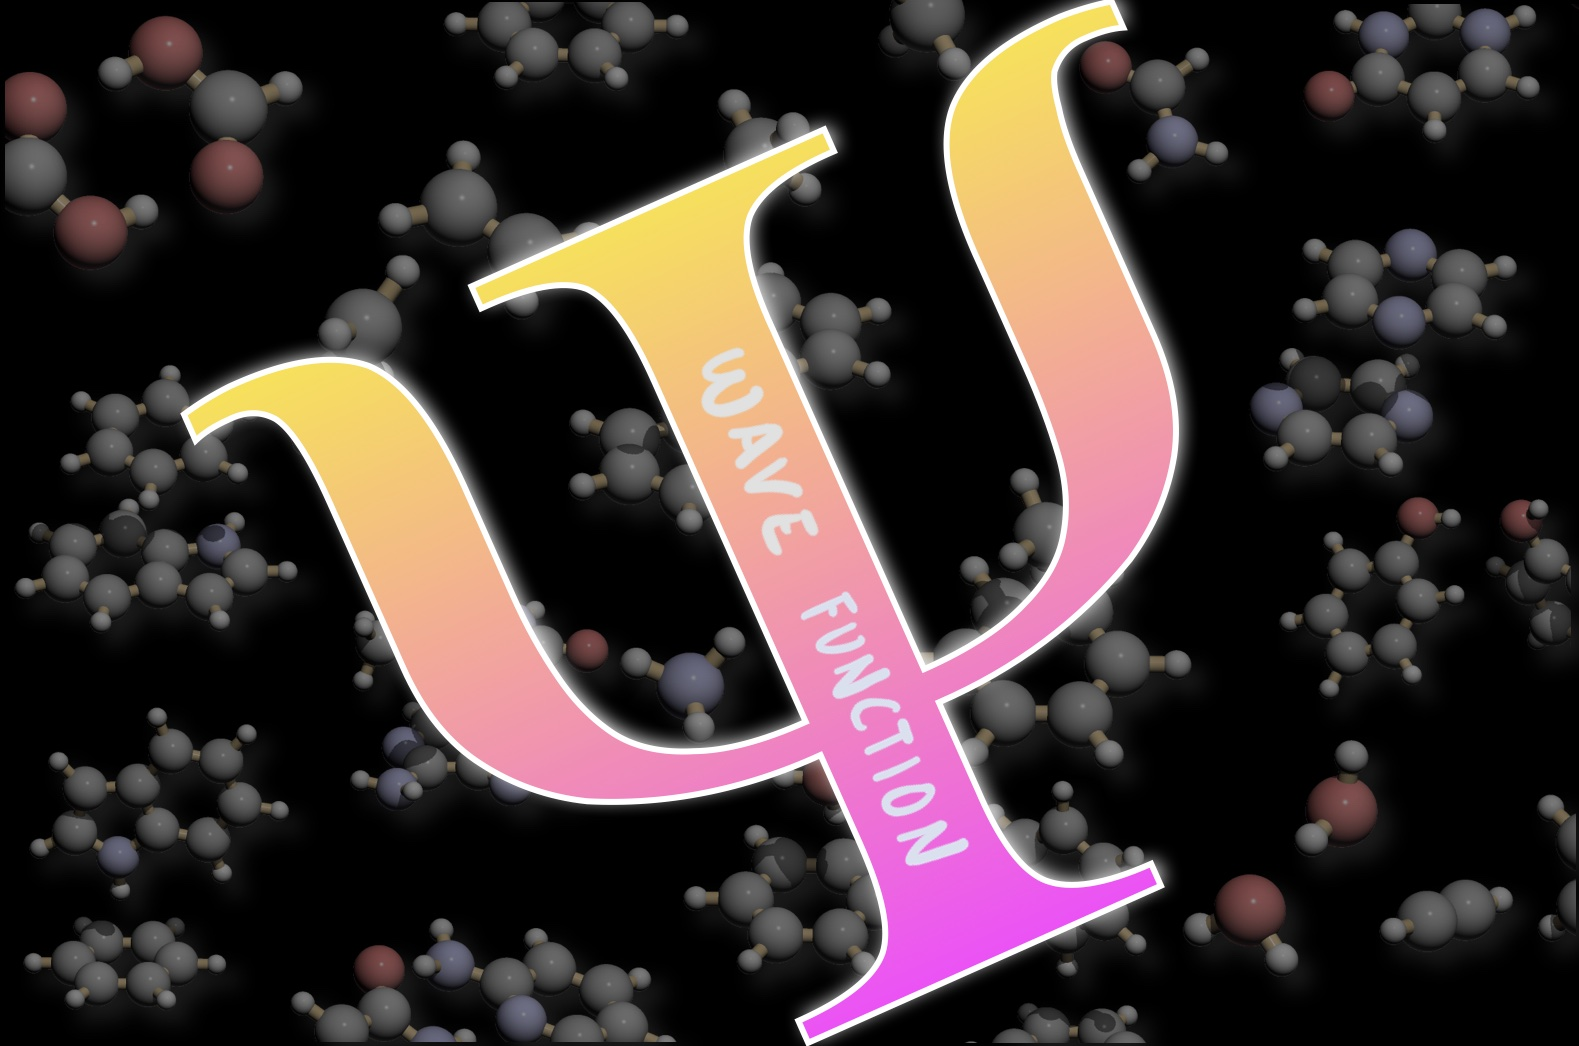
\includegraphics[width=0.8\linewidth]{./img/OEP_Figures.000} \end{center}

This textbook is the official textbook for the Physical Chemistry 2 Course (CHM 3002) at Florida Tech.

The instructor for this course and author of this textbook is Dr.~Roberto Peverati.

\textbf{Contacts}: \href{mailto:rpeverati@fit.edu}{\nolinkurl{rpeverati@fit.edu}}, Office: OPS 333, (321) 674-7735

Chemistry Program, Department of Biomedical and Chemical Engineering and Science
Florida Institute of Technology, Melbourne, FL.

\begin{quote}
This live open textbook is distributed under the \href{https://creativecommons.org/licenses/by-sa/4.0/}{CC-BY-SA 4.0 License} and it was funded by the Florida Tech Open Educational Resources Grant Program: A Collaboration of the Teaching Council, eEducation, and the Evans Library.
\end{quote}

\hypertarget{how-to-use-this-book}{%
\section*{How to use this book}\label{how-to-use-this-book}}
\addcontentsline{toc}{section}{How to use this book}

If you have taken P-Chem 1 at Florida Tech in the Fall Semester 2020, you should already be familiar with this format. Everything we did with the Live Textbook of P-Chem 1 in FS2020 will be happening this semester with P-Chem 2. Please read this book carefully, since everything that will be in your exams is explained here.
Since this book is specifically tailored for the CHM 3002 course at Florida Tech, there are no superfluous parts. In other words, everything in it might be subject to question in the quizzes and the final exam.

\begin{quote}
Definitions and exercises are usually numbered and are highlighted in the text in this format (lighter grey, indented, and following a grey vertical bar). Please study the definitions carefully since they are fundamental concepts that will be used several times in the remainder of the text, and they will be subject to quizzes and exams. Exercises are essential for cementing the concepts, and you should attempt to execute them first without looking at the solution. Even if you were able to solve an exercise on your own, always read the solution after, since it might contain additional explanations expanding the main concepts in the text.
\end{quote}

Navigating the book should be straightforward. On each page, there is a useful sidebar on the left that gives you an overview of all chapters, and a toolbar at the top with important tools. Arrows to shift between chapters might also be present, depending on your browser. If you are old-school and prefer a pdf, you can download a printout by clicking on the toolbar's corresponding icon. If you are \emph{really} old-school and prefer a printed book, the best solution is to download the pdf and print it yourself. It is a LaTeX book, and I can promise you it will look good on paper. However, I cannot provide physical copies to each student. In the toolbar, you will find a useful search box that is capable of searching the entire book. The most adventurous will find in the toolbar a link to the raw GitHub source code. Feel free to head on \href{https://github.com/peverati/PChem2}{over there} and fork the book.

Each chapter of this book represents one week of work in the classroom and at home. The sidebar on the left will reflect your syllabus, as well as the main structure of the class on Canvas. The book is a live document, which means it will be updated throughout the semester with new material. While you are not required to check it every day, you might want to review each week's chapter before the lecture on Friday.

\begin{quote}
If you spot a mistake or a typo, contact Dr.~Peverati via \href{mailto:rpeverati@fit.edu}{email} and you will receive a credit of up to three points towards your final score, once the typo has been verified and corrected.
\end{quote}

\cleardoublepage
\pagenumbering{arabic}

\hypertarget{Motivation}{%
\chapter{The Motivation for Quantum Mechanics}\label{Motivation}}

\hypertarget{introduction}{%
\section{Introduction}\label{introduction}}

Quantum mechanics is an important intellectual achievement of the 20th century. It is one of the more sophisticated field in physics that has affected our understanding of nano-meter length scale systems important for chemistry, materials, optics, and electronics. The existence of orbitals and energy levels in atoms can only be explained by quantum mechanics. Quantum mechanics can explain the behaviors of insulators, conductors, semi-conductors, and giant magneto-resistance. It can explain the quantization of light and its particle nature in addition to its wave nature. Quantum mechanics can also explain the radiation of hot body, and its change of color with respect to temperature. It explains the presence of holes and the transport of holes and electrons in electronic devices.
Quantum mechanics has played an important role in photonics, quantum electronics, and micro-electronics. But many more emerging technologies require the understanding of quantum mechanics; and hence, it is important that scientists and engineers understand quantum mechanics better. One area is nano-technologies due to the recent advent of nano-fabrication techniques. Consequently, nano-meter size systems are more common place. In electronics, as transistor devices become smaller, how the electrons move through the device is quite different from when the devices are bigger: nano-electronic transport is quite different from micro-electronic transport.
The quantization of electromagnetic field is important in the area of nano-optics and quantum optics. It explains how photons interact with atomic systems or materials. It also allows the use of electromagnetic or optical field to carry quantum information. Moreover, quantum mechanics is also needed to understand the interaction of photons with materials in solar cells, as well as many topics in material science.
When two objects are placed close together, they experience a force called the Casimir force that can only be explained by quantum mechanics. This is important for the understanding of micro/nano-electromechanical sensor systems (M/NEMS). Moreover, the understanding of spins is important in spintronics, another emerging technology where giant magneto-resistance, tunneling magneto-resistance, and spin transfer torque are being used.
Quantum mechanics is also giving rise to the areas of quantum information, quantum communication, quantum cryptography, and quantum computing. It is seen that the richness
of quantum physics will greatly affect the future generation technologies in many aspects.

\hypertarget{quantum-mechanics-is-bizarre}{%
\section{Quantum Mechanics is Bizarre}\label{quantum-mechanics-is-bizarre}}

The development of quantum mechanics is a great intellectual achievement, but at the same time, it is bizarre. The reason is that quantum mechanics is quite different from classical physics. The development of quantum mechanics is likened to watching two players having a game of chess, but the watchers have not a clue as to what the rules of the game are. By observations, and conjectures, finally the rules of the game are outlined. Often, equations are conjectured like conjurors pulling tricks out of a hat to match experimental observations. It is the interpretations of these equations that can be quite bizarre.
Quantum mechanics equations were postulated to explain experimental observations, but the deeper meanings of the equations often confused even the most gifted. Even though Einstein received the Nobel prize for his work on the photo-electric effect that confirmed that light energy is quantized, he himself was not totally at ease with the development of quantum mechanics as charted by the younger physicists. He was never comfortable with the probabilistic interpretation of quantum mechanics by Born and the Heisenberg uncertainty principle: ``God doesn't play dice,'' was his statement assailing the probabilistic interpretation. He proposed ``hidden variables'' to explain the random nature of many experimental observations. He was thought of as the ``old fool'' by the younger physicists during his time.
Schrödinger came up with the bizarre ``Schrödinger cat paradox'' that showed the struggle that physicists had with quantum mechanics's interpretation. But with today's understanding of quantum mechanics, the paradox is a thing of yesteryear.
The latest twist to the interpretation in quantum mechanics is the parallel universe view that explains the multitude of outcomes of the prediction of quantum mechanics. All outcomes are possible, but with each outcome occurring in different universes that exist in parallel with respect to each other.\footnote{This section was adapted in part from Prof.~Weng Cho CHEW's Quantum Mechanics Made Simple Lecture Notes available \href{http://wcchew.ece.illinois.edu/chew/course/qmall20121005.pdf}{here}.}

The development of quantum mechanics was initially motivated by two observations which demonstrated the inadeqacy of classical physics. These are the ``ultraviolet catastrophe'' and the photoelectric effect.

\hypertarget{the-ultraviolet-catastrophe}{%
\section{The Ultraviolet Catastrophe}\label{the-ultraviolet-catastrophe}}

A blackbody is an idealized object which absorbs and emits all frequencies. Classical physics can be used to derive an equation which describes the intensity of blackbody radiation as a function of frequency for a fixed temperature--the result is known as the Rayleigh-Jeans law. Although the Rayleigh-Jeans law works for low frequencies, it diverges as \(\nu^2\); this divergence for high frequencies is called the ultraviolet catastrophe.
Max Planck explained the blackbody radiation in 1900 by assuming that the energies of the oscillations of electrons which gave rise to the radiation must be proportional to integral multiples of the frequency, i.e.,

\begin{equation}
E = n h \nu
\label{eq:uvcat}
\end{equation}

Using statistical mechanics, Planck derived an equation similar to the Rayleigh-Jeans equation, but with the adjustable parameter \(h\). Planck found that for \(h = 6.626 \times 10^{-34} \; \text{J s}\), the experimental data could be reproduced. Nevertheless, Planck could not offer a good justification for his assumption of energy quantization. Physicicsts did not take this energy quantization idea seriously until Einstein invoked a similar assumption to explain the photoelectric effect.

\hypertarget{the-photoelectric-effect}{%
\section{The Photoelectric Effect}\label{the-photoelectric-effect}}

In 1886 and 1887, Heinrich Hertz discovered that ultraviolet light can cause electrons to be ejected from a metal surface. According to the classical wave theory of light, the intensity of the light determines the amplitude of the wave, and so a greater light intensity should cause the electrons on the metal to oscillate more violently and to be ejected with a greater kinetic energy. In contrast, the experiment showed that the kinetic energy of the ejected electrons depends on the frequency of the light. The light intensity affects only the number of ejected electrons and not their kinetic energies.
Einstein tackled the problem of the photoelectric effect in 1905. Instead of assuming that the electronic oscillators had energies given by Planck's formula, eq. \eqref{eq:uvcat}, Einstein assumed that the radiation itself consisted of packets of energy \(E = h \nu\), which are now called photons. Einstein successfully explained the photoelectric effect using this assumption, and he calculated a value of \(h\) close to that obtained by Planck.

Two years later, Einstein showed that not only is light quantized, but so are atomic vibrations. Classical physics predicts that the molar heat capacity at constant volume (\(C_V\)) of a crystal is \(3 R\), where \(R\) is the molar gas constant. This works well for high temperatures, but for low temperatures \(C_V\) actually falls to zero. Einstein was able to explain this result by assuming that the oscillations of atoms about their equilibrium positions are quantized according to \(E = n h \nu\), Planck's quantization condition for electronic oscillators. This demonstrated that the energy quantization concept was important even for a system of atoms in a crystal, which should be well-modeled by a system of masses and springs (i.e., by classical mechanics).

\hypertarget{wave-particle-duality}{%
\section{Wave-Particle Duality}\label{wave-particle-duality}}

Einstein had shown that the momentum of a photon is

\begin{equation}
p = \frac{h}{\lambda}.
\label{eq:wp1}
\end{equation}

This can be easily shown as follows. Assuming \(E = h \nu\) for a photon and \(\lambda \nu = c\) for an electromagnetic wave, we obtain

\begin{equation}
E = \frac{h c}{\lambda}
\label{eq:wp2}
\end{equation}

Now we use Einstein's relativity result, \(E = m c^2\), and the definition of mementum \(p=mc\), to find:
\begin{equation}
\lambda = \frac{h}{p},
\label{eq:wp3}
\end{equation}

which is equivalent to eq. \eqref{eq:wp1}. Note that \(m\) refers to the relativistic mass, not the rest mass, since the rest mass of a photon is zero. Since light can behave both as a wave (it can be diffracted, and it has a wavelength), and as a particle (it contains packets of energy \(h \nu\)), de Broglie reasoned in 1924 that matter also can exhibit this wave-particle duality. He further reasoned that matter would obey the same eq. \eqref{eq:wp3} as light. In 1927, Davisson and Germer observed diffraction patterns by bombarding metals with electrons, confirming de Broglie's proposition.\footnote{The previous 3 sections were adapted in part from Prof.~C. David Sherrill's A Brief Review of Elementary Quantum Chemistry Notes available \href{http://vergil.chemistry.gatech.edu/notes/quantrev/node1.html}{here}.}

Rewriting the previous equations in terms of the wave vector, \(k=\frac{2\pi}{\lambda}\), and the angular frequency, \(\omega=2\pi\nu\), we obtain the following two equations

\begin{equation}
\begin{aligned}
p &= \hbar k \\
E &= \hbar \omega,
\end{aligned}
\label{eq:wp1b}
\end{equation}

which are known as \textbf{de Broglie's equations}. We will use those equation to develop wave mechanics in the next chapters.

\hypertarget{Classical}{%
\chapter{Classical Mechanics}\label{Classical}}

Quantum mechanics cannot be derived from classical mechanics, but classical mechanics can inspire quantum mechanics. Quantum mechanics is richer and more sophisticated than classical mechanics. Quantum mechanics was developed during the period when physicists had rich knowledge of classical mechanics. In order to better understand how quantum mechanics was developed in this environment, it is better to understand some fundamental concepts in classical mechanics. Classical mechanics can be considered as a special case of quantum mechanics. We will review some classical mechanics concepts here.

\hypertarget{newtonian-formulation}{%
\section{Newtonian Formulation}\label{newtonian-formulation}}

In classical mechanics, a particle moving in the presence of potential \(V(q)\) will experience a force given by:

\begin{equation}
F(q) = -\frac{dV(q)}{dq},
\label{eq:class1}
\end{equation}

where \(q\) represents the coordinate or the position of the particle. Hence, the particle can be described by the equations of motion:

\begin{equation}
\frac{dp}{dt} = \dot{p} = F(q) = -\frac{dV (q)}{dq},\quad \frac{dq}{dt} =\dot{q}= \frac{p}{m}.
\label{eq:class2}
\end{equation}

For example, when a particle is attached to a spring and moves along a frictionless surface, the force the particle experiences is \(F(q) = -kq\) where \(k\) is the spring constant. Then the equations of motion of this particle are

\begin{equation}
\dot{p}=-kq,\quad \dot{q}=p/m
\label{eq:class3}
\end{equation}

Given \(p\) and \(q\) at some initial time \(t_0\), one can integrate \eqref{eq:class2} or \eqref{eq:class3} to obtain \(p\) and \(q\) for all later time. Notice that only two variables \(p\) and \(q\) are sufficient to describe the state of a particle. These equations of motion are essentially derived using Newton's law. However, there are at least two other methods of deriving these equations of motion, which are described below.

\hypertarget{lagrangian-formulation}{%
\section{Lagrangian Formulation}\label{lagrangian-formulation}}

Another way to derive the equations of motion for classical mechanics is via the use of the Lagrangian and the principle of least action. The Lagrangian formulation is obtained by starting from the definition of the Lagrangian of the system:

\begin{equation}
L = K - V,
\label{eq:lag1}
\end{equation}

where \(K\) is the kinetic energy, and \(V\) is the potential energy. Both are expressed in terms of coordinates \((q,\dot{q}\)) where \(q\) \(\in\) \(\mathbb{R}^{n}\) is the position vector and \(\dot{q}\) \(\in\) \(\mathbb{R}^{n}\) is the velocity vector. Notice that for a fixed time, \(t\), \(q\) and \(\dot{q}\) are independent variables, since \(\dot{q}\) cannot be derived from \(q\) alone.

The time integral of the Lagrangian is called the \textbf{action}, and is defined as:

\begin{equation}
S = \int_{t_1}^{t_2} L\, dt,
\label{eq:lag2}
\end{equation}

which is a functional: it takes in the Lagrangian function for all times between \(t_1\) and \(t_2\) and returns a scalar value. The equations of motion can be derived from the principle of least action,\footnote{Sometimes also called principle of stationary action, or variational principle, or Hamilton's principle.} which states that the true evolution of a system \(q(t)\) described by the coordinate \(q\) between two specified states \(q_1 = q(t_1)\) and \(q_2 = q(t_2)\) at two specified times \(t_1\) and \(t_2\) is a stationary point of the action functional. For a stationary point:

\begin{equation}
\delta     S = \frac{dS}{dq}= 0
\label{eq:lag3}
\end{equation}

Requiring that the true trajectory \(q(t)\) be a stationary point of the action functional \(S\) we obtain the equation of motion (figure \ref{fig:Fig1c2}\footnote{This diagram is taken from \href{https://en.wikipedia.org}{Wikipedia} by user Maschen, and distributed under CC0 license}). This can be achieved applying classical variational calculus to the variation of the action integral \(S\) under perturbations of the path \(q(t)\), eq. \eqref{eq:lag3}. The resulting equation of motion (or set of equations in the case of many dimensions) is sometimes also called the Euler---Lagrange equation:\footnote{The mathematical derivation of the Euler---Lagrange equaiton is rather long and unimportant at this stage. For the curious, it can be found \href{https://en.wikipedia.org/wiki/Euler–Lagrange_equation}{here}.}

\begin{equation}
\frac{d}{dt}\left(\frac{\partial L}{\partial\dot q}\right)=\frac{\partial L}{\partial q}.
\label{eq:lag4}
\end{equation}

\begin{figure}

{\centering 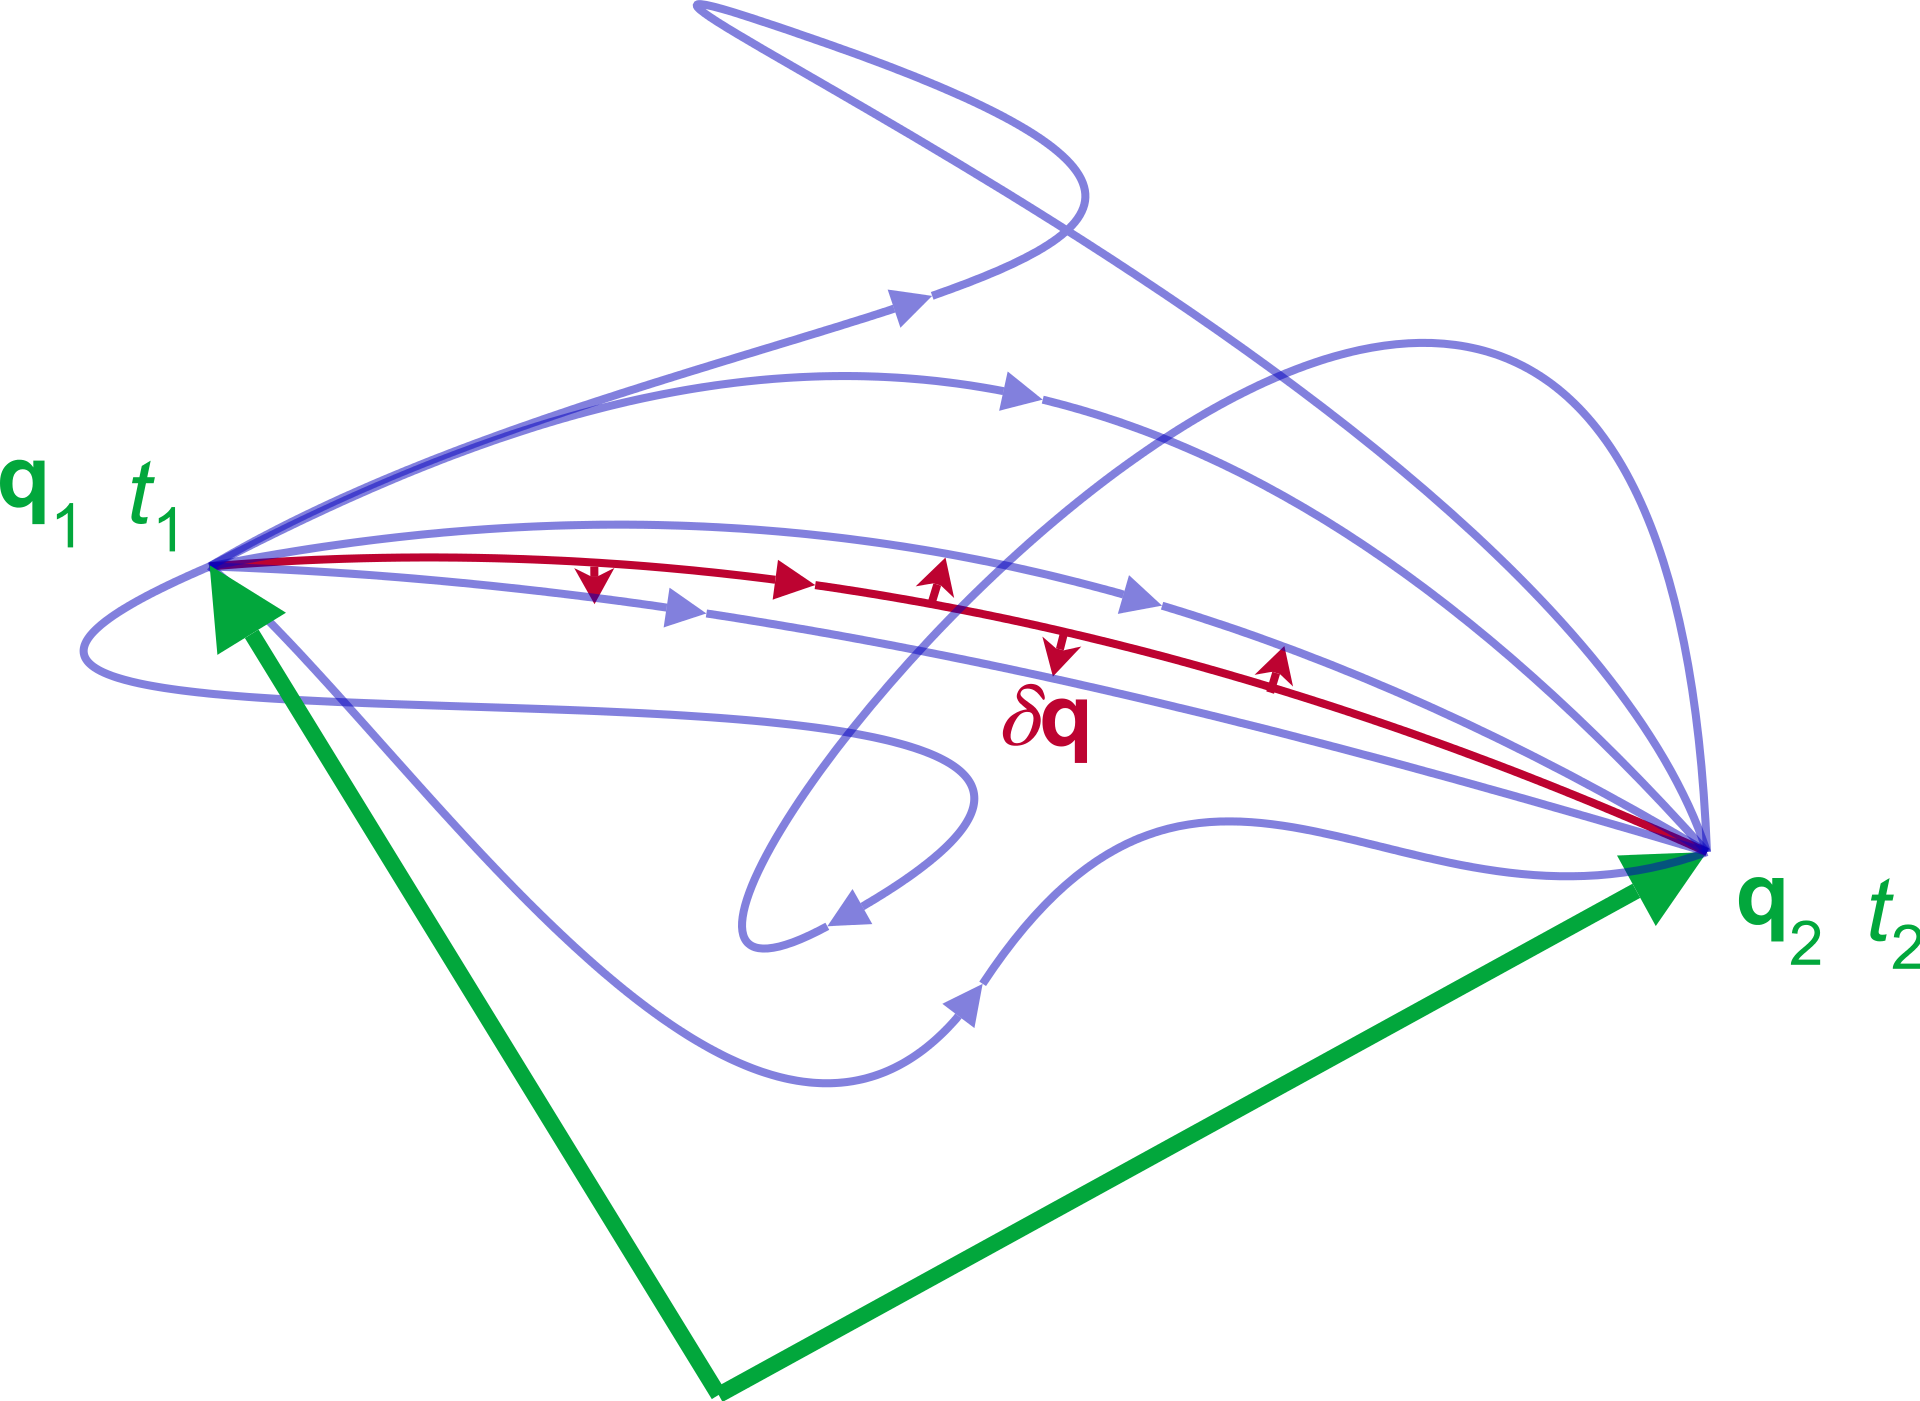
\includegraphics[width=0.7\linewidth]{./img/OEP_wiki1} 

}

\caption{Principle of least action: As the system evolves, q traces a path through configuration space (only some are shown). The path taken by the system (red) has a stationary action under small changes in the configuration of the system.}\label{fig:Fig1c2}
\end{figure}

\hypertarget{hamiltonian-mechanics}{%
\section{Hamiltonian mechanics}\label{hamiltonian-mechanics}}

A third way of obtaining the equation of motion is Hamiltonian mechanics, which uses the generalized momentum in place of velocity as a coordinate. The generalized momentum is defined in terms of the Lagrangian and the coordinates \((q,\dot{q})\):

\begin{equation} 
p = \frac{\partial L}{\partial\dot q}.
\label{eq:ham1}
\end{equation}

The Hamiltonian is defined from the Lagrangian by applying a Legendre transformation as:\footnote{We have already encountered Legendre transform in \href{https://peverati.github.io/pchem1/Potentials.html\#thermpot}{The Live Textbook of Physical Chemistry 1} when transforming from the thermodynamic energy to any of the other thermodynamic potentials.}

\begin{equation} 
H(p,q) = p\dot{q} - L(q,\dot{q}),
\label{eq:ham2}
\end{equation}

The Lagrangian equation of motion becomes a pair of equations known as the Hamiltonian system of equations:

\begin{equation} 
\begin{aligned}
\dot{p}=\frac{dp}{dt} &= -\frac{\partial H}{\partial q} \\
\dot{q}=\frac{dq}{dt} &= +\frac{\partial H}{\partial p},
\end{aligned}
\label{eq:ham3}
\end{equation}

where \(H=H(q,p,t)\) is the Hamiltonian of the system, which often corresponds to its total energy. For a closed system, it is the sum of the kinetic and potential energy in the system:

\begin{equation}
H = K + V.
\label{eq:hamdef}
\end{equation}

Notice the difference between the Hamiltonian, eq. \eqref{eq:hamdef}, and the Lagrangian, eq. \eqref{eq:lag1}. In Newtonian mechanics, the time evolution is obtained by computing the total force being exerted on each particle of the system, and from Newton's second law, the time evolutions of both position and velocity are computed. In contrast, in Hamiltonian mechanics, the time evolution is obtained by computing the Hamiltonian of the system in the generalized momenta and inserting it into Hamilton's equations. This approach is equivalent to the one used in Lagrangian mechanics, since the Hamiltonian is the Legendre transform of the Lagrangian. The main motivation to use Hamiltonian mechanics instead of Lagrangian mechanics comes from the more simple description of complex dynamic systems.

\begin{quote}
\begin{example}
\protect\hypertarget{exm:hamex1}{}{\label{exm:hamex1} }\emph{Basic Interpretation of Hamiltonian Mechanics}

A simple interpretation of Hamiltonian mechanics comes from its application on a one-dimensional system consisting of one particle of mass \(m\). The Hamiltonian can represent the total energy of the system, which is the sum of kinetic and potential energy.

\begin{equation}
\begin{aligned}
H &= K+V \\
K &={\frac {p^{2}}{2m}},\quad V=V(q),
\end{aligned}
\label{eq:ham4}
\end{equation}

where \(q\) is the space coordinate and \(p=m\dot{q}\) is the momentum. Then
\(K\) is a function of \(p\) alone, while \(V\) is a function of \(q\) alone.

In this example, the time derivative of the momentum \(p\) equals the Newtonian force, and so the first Hamilton equation means that the force equals the negative gradient of potential energy:

\begin{equation}
\text{Newtonian force:}\qquad \frac{dp}{dt} = -\frac{\partial H}{\partial q}= -\frac{\partial V(q)}{\partial q},
\label{eq:ham5}
\end{equation}

which is exactly the first equation of motion in eq. \eqref{eq:class2} of Newtonian mechanics. Notice that this equaiton could have been easily obtained in the Lagrangian formulation by writing the Lagrangian \eqref{eq:lag1}, and using the Euler-Lagrange equation, eq. \eqref{eq:lag4}.
The time derivative of \(q\) is the velocity, and so the second Hamilton equation means that the particle's velocity equals the derivative of its kinetic energy with respect to its momentum:

\begin{equation}
\text{Velocity:}\qquad \frac{dq}{dt} = \frac{\partial K}{\partial p} = \frac{\partial \left(\frac{p^2}{2m}\right)}{\partial p} = \frac{p}{m},
\label{eq:ham6}
\end{equation}

which is exactly the second equation of motion in eq. \eqref{eq:class2} of Newtonian mechanics.
\end{example}
\end{quote}

\hypertarget{Schrodinger}{%
\chapter{The Schrödinger Equation}\label{Schrodinger}}

In 1925, Erwin Schrödinger and Werner Heisenberg independently developed the new quantum theory. Schrödinger's method involves partial differential equations, whereas Heisenberg's method employs matrices; however, a year later the two methods were shown to be mathematically equivalent. Most textbooks begin with Schrödinger's equation, since it seems to have a better physical interpretation via the classical wave equation. Indeed, the Schrödinger equation can be viewed as a form of the wave equation applied to matter waves.

\hypertarget{the-time-independent-schruxf6dinger-equation}{%
\section{The Time-Independent Schrödinger Equation}\label{the-time-independent-schruxf6dinger-equation}}

We can start the derivation of the single-particle time-independent Schrödinger equation (TISEq) from the equation that describes the motion of a wave in classical mechanics:

\begin{equation}
\psi(x,t)=\exp[i(kx-\omega t)],
\label{eq:sch1}
\end{equation}

where \(x\) is the position, \(t\) is time, \(k=\frac{2\pi}{\lambda}\) is the wave vector, and \(\omega=2\pi\nu\) is the angular frequency of the wave. If we are not concerned with the time evolution, we can consider uniquely the derivatives of eq. \eqref{eq:sch1} with respect to the location, which are:

\begin{equation}
\begin{aligned}
\frac{\partial \psi}{\partial x} &=ik\exp[i(kx-\omega t)] = ik\psi, \\
\frac{\partial^2 \psi}{\partial x^2} &=i^2k^2\exp[i(kx-\omega t)] = -k^2\psi,
\end{aligned}
\label{eq:sch2}
\end{equation}

where we have used the fact that \(i^2=-1\).

Assuming that particles behaves as wave---as proven by de Broglie's we can now use the first of de Broglie's equation, eq. \eqref{eq:wp1b}, we can replace \(k=\frac{p}{\hbar}\) to obtain:

\begin{equation}
\frac{\partial^2 \psi}{\partial x^2} = -\frac{p^2\psi}{\hbar^2},
\label{eq:sch3}
\end{equation}

which can be rearranged to:

\begin{equation}
p^2 \psi = -\hbar^2 \frac{\partial^2 \psi}{\partial x^2}.
\label{eq:sch4}
\end{equation}

The total energy associated with a wave moving in space is simply the sum of its kinetic and potential energies:

\begin{equation}
E = \frac {p^{2}}{2m} + V(x),
\label{eq:sch5}
\end{equation}

from which we can obtain:

\begin{equation}
p^2 = 2m[E - V(x)],
\label{eq:sch6}
\end{equation}

which we can then replace into eq. \eqref{eq:sch4} to obtain:

\begin{equation}
2m[E-V(x)]\psi = - \hbar^2 \frac{\partial^2 \psi}{\partial x^2},
\label{eq:sch7}
\end{equation}

which can then be rearranged to the famous \textbf{time-independent Schrödinger equation (TISEq)}:

\begin{equation}
- \frac{\hbar^2}{2m} \frac{\partial^2 \psi}{\partial x^2} + V(x) \psi = E\psi,
\label{eq:TISEq}
\end{equation}

A two-body problem can also be treated by this equation if the mass \(m\) is replaced with a reduced mass \(\mu = \frac{m_1 m_2}{m_1+m_2}\).

\hypertarget{the-time-dependent-schruxf6dinger-equation}{%
\section{The Time-Dependent Schrödinger Equation}\label{the-time-dependent-schruxf6dinger-equation}}

Unfortunately, the analogy with the classical wave equation that allowed us to obtain the TISEq in the previous section cannot be extended to the time domain by considering the equation that involves the partial first derivative with respect to time. Schrödinger himself presented his time-independent equation first, and then went back and postulated the more general time-dependent equation. We are following here the same strategy and just give the time-independent variable as a postulate. The single-particle time-dependent Schrödinger equation is:

\begin{equation}
i\hbar\frac{\partial \psi(x,t)}{\partial t}=-\frac{\hbar^2}{2m} \frac{\partial^2 \psi(x,t)}{\partial x^2}+V(x)\psi(x,t)
\label{eq:TDSEq}
\end{equation}

where \(V \in \mathbb{R}^{n}\) represents the potential energy of the system.
Obviously, the time-dependent equation can be used to derive the time-independent equation. If we write the wavefunction as a product of spatial and temporal terms, \(\psi(x, t) = \psi(x) f(t)\), then equation \eqref{eq:TDSEq} becomes:

\begin{equation}
\psi(x) i \hbar \frac{df(t)}{dt} = f(t) \left[-\frac{\hbar^2}{2m} \frac{\partial^2}{\partial x^2} + V(x) \right] \psi(x),
\label{eq:TDSEq2}
\end{equation}

which can be rearranged to:

\begin{equation}
\frac{i \hbar}{f(t)} \frac{df(t)}{dt} = \frac{1}{\psi(x)} \left[-\frac{\hbar^2}{2m} \frac{\partial^2}{\partial x^2} + V(x) \right] \psi(x).
\label{eq:TDSEq3}
\end{equation}

Since the left-hand side of eq. \eqref{eq:TDSEq3} is a function of \(t\) only and the right hand side is a function of \(x\) only, the two sides must equal a constant. If we tentatively designate this constant \(E\) (since the right-hand side clearly must have the dimensions of energy), then we extract two ordinary differential equations, namely:

\begin{equation}
\frac{1}{f(t)} \frac{df(t)}{dt} = - \frac{i E}{\hbar}
\label{eq:TDSEq4}
\end{equation}

and:
\begin{equation}
-\frac{\hbar^2}{2m} \frac{\partial^2\psi(x)}{\partial x^2} + V(x) \psi(x) =
E \psi(x).
\label{eq:TDSEq5}
\end{equation}

The latter equation is the TISEq. The former equation is easily solved to yield

\begin{equation}
f(t) = e^{-iEt / \hbar}
\label{eq:TDSEq6}
\end{equation}

The solutions of eq. \eqref{eq:TDSEq6}, \(f(t)\), are purely oscillatory, since \(f(t)\) never changes in magnitude. Thus if:

\begin{equation}
\psi(x, t) = \psi(x) \exp\left(\frac{-iEt}{\hbar}\right),
\label{eq:TDSEq6b}
\end{equation}

then the total wave function \(\psi(x, t)\) differs from \(\psi(x)\) only by a phase factor of constant magnitude. There are some interesting consequences of this. First of all, the quantity \(\vert \psi(x, t) \vert^2\) is time independent, as we can easily show:

\begin{equation}
\vert \psi(x, t) \vert^2 = \psi^{*}(x, t) \psi(x, t)=
\exp\left(\frac{iEt}{\hbar}\right)\exp\left(\frac{-iEt}{\hbar}\right)=
\psi^{*}(x) \psi(x).
\label{eq:TDSEq7}
\end{equation}

Wave functions of the form of eq. \eqref{eq:TDSEq6b} are called stationary states. The state \(\psi(x, t)\) is ``stationary,'' but the particle it describes is not!
Of course eq. \eqref{eq:TDSEq6} represents only a particular solution to the time-dependent Schrödinger equation. The general solution is, in general, much more complicated.\footnote{This sections was adapted in part from Prof.~C. David Sherrill's A Brief Review of Elementary Quantum Chemistry Notes available \href{http://vergil.chemistry.gatech.edu/notes/quantrev/node1.html}{here}.}

\begin{equation}
\psi({\bf r}, t) = \sum_i c_i e^{-iE_it / \hbar} \psi_i({\bf r})
\end{equation}

\hypertarget{Models}{%
\chapter{Analytically Soluble Models}\label{Models}}

The TISEq can be solved analytically only in a few special cases. In this section, we will analyze the main four. Luckily, we can use these solutions to explain most of the effects in chemistry since we can combine them to describe the hydrogen atom upon which we can build more complex chemical systems, as we will show in the next chapters.

\hypertarget{the-free-particle}{%
\section{The Free Particle}\label{the-free-particle}}

By definition, the particle does not feel any external force, therefore \(V(x)=0\), and the TISEq is written simply:

\begin{equation}
- \frac{\hbar^2}{2m} \frac{d^2\psi}{dx^2} = E \psi(x).
\label{eq:FP1}
\end{equation}

This equation can be rearranged to:

\begin{equation}
\frac{d^2\psi}{dx^2} =- \frac{2mE}{\hbar^2} \psi(x),
\label{eq:FP2}
\end{equation}

which corresponds to a mathematical problem where the second derivative of a function should be equal to a constant, \(- \frac{2mE}{\hbar^2}\) multiplied by the function itself. Such a problem is easily solved by the function:

\begin{equation}
\psi(x) = A \exp(\pm ikx).
\label{eq:FP3}
\end{equation}

The first and second derivatives of this function are:

\begin{equation}
\begin{aligned}
\frac{d \psi(x)}{dx} &= \pm ik A \exp(\pm ikx) = \pm ik \psi(x) \\
\frac{d^2 \psi(x)}{dx^2} &= \mp k^2  A \exp(\pm ikx) = -(\pm k^2) \psi(x). 
\end{aligned}
\label{eq:FP4}
\end{equation}

Comparing the second derivative in eq. \eqref{eq:FP4} with eq. \eqref{eq:FP2}, we immediately see that if we set:

\begin{equation}
k^2 = \frac{2mE}{\hbar^2},
\label{eq:FP5}
\end{equation}

we solve the original differential equation. Considering de Broglie's equation, eq. \eqref{eq:wp1b}, we can replace \(k=\frac{p}{\hbar}\), to obtain:

\begin{equation}
E = \frac{k^2 \hbar^2}{2m} = \frac{p^2}{2m},
\label{eq:FP6}
\end{equation}

which is exactly the classical value of the kinetic energy of a free particle moving in one direction of space. Since the function in eq. \eqref{eq:FP3} solves the Schrödinger equation for the free particle, it is called an \emph{eigenfunction} (or \emph{eigenstate}) of the TISEq. The energy result of eq. \eqref{eq:FP6} is called \emph{eigenvalue} of the TISEq. Notice that, since \(k\) is continuous in the eigenfunction, the energy eigenvalue is also continuous (i.e., all values of \(E\) are acceptable).

\hypertarget{rigidrotor}{%
\section{The Particle in a Box}\label{rigidrotor}}

Now we can consider a particle constrained to move in a single dimension, under the influence of a potential \(V(x)\) which is zero for \(0 \leq x \leq a\) and infinite elsewhere. Since the wavefunction is not allowed to become infinite, it must have a value of zero where \(V(x)\) is infinite, so \(\psi(x)\) is nonzero only within \([0,a]\). The Schrödinger equation is thus:

\begin{equation}
- \frac{\hbar^2}{2m} \frac{d^2\psi}{dx^2} = E \psi(x)
\qquad 0 \leq x \leq a.
\label{eq:PIB1}
\end{equation}

In other words, inside the box \(\psi(x)\) describes a free particle, but outside the box \(\psi(x)=0\). Since the Schrödinger equation involves derivatives, the function that solves it, \(\psi(x)\), must be everywhere continuous and everywhere continuously differentiable. This fact means that the value of the wave function at the two extremes must be equal to zero:

\begin{equation}
\psi(0)=\psi(a)=0.
\label{eq:PIB2}
\end{equation}

Inside the box we can use Euler's formula to write the wave function as a linear combination of the positive and negative solutions:

\begin{equation}
\psi(x)=A \exp(\pm ix)=A \sin kx + B \cos kx,
\label{eq:PIB3}
\end{equation}

where \(A\) and \(B\) are constants that we need to determine using the two constraints in eq. \eqref{eq:PIB2}. For \(B\) it is straightforward to see that:

\begin{equation}
\psi(0)= 0 + B =0 \; \implies \; B=0.
\label{eq:PIB4}
\end{equation}

For \(A\) we have:

\begin{equation}
\psi(a)= A\sin ka = 0,
\label{eq:PIB5}
\end{equation}

which is trivially solved by \(A=0\), or by the more interesting condition of \(ka=n\pi\). The trivial solution corresponds to a wave function uniformly equal to zero everywhere. This wave function is uninteresting, since it describes no particles in no boxes. The second set of solutions, however, is very interesting, since we can write it as:

\begin{equation}
\psi_n(x)= A\sin\left(\frac{n\pi x}{a} \right)\quad n=1,2,\ldots,\infty,
\label{eq:PIB6}
\end{equation}

which represents an infinite set of functions, \(\psi_n(x)\), determined by a positive integer number \(n\), called \emph{quantum number}. Since these functions solve the TISEq, they are also called \emph{eigenfunctions}, but they are not a continuous set, unlike in the previous case. To calculate the energy eigenvalues, we can replace \eqref{eq:PIB6} into eq. \eqref{eq:PIB1}, to obtain:

\begin{equation}
E_n = \frac{h^2 n^2}{8 m a^2} \quad n=1,2,\ldots,\infty.
\label{eq:PIB7}
\end{equation}

A few interesting considerations can be made from the results of eq. \eqref{eq:PIB7}. First, although there is an infinite number of acceptable values of the energy (eigenvalues), these values are not continuous. Second, the lowest value of the energy is not zero, and it depends on the size of the box, \(a\), since:

\begin{equation}
E_1 = \frac{h^2 }{8 m a^2} \neq 0.
\label{eq:PIB8}
\end{equation}

This value is called \emph{zero-point energy (ZPE)}, and is a purely quantum mechanical effect. Notice that we did not solve for the constant \(A\). This task is not straightforward, and it can be achieved by requiring the wave function to describe one particle exclusively (we will come back to this task after chapter 7). Extending the problem to three dimensions is relatively straightforward, resulting in a set of three separate quantum numbers (one for each of the 3-dimensional coordinate \(n_x,n_y,n_z\)).

\hypertarget{the-harmonic-oscillator}{%
\section{The Harmonic Oscillator}\label{the-harmonic-oscillator}}

We now consider a particle subject to a restoring force \(F = -kx\), as might arise for a mass-spring system obeying Hooke's Law. The potential is then:

\begin{equation}
V(x) = - \int_{-\infty}^{\infty} (-kx) dx = V_0 + \frac{1}{2} kx^2.
\label{eq:HO1}
\end{equation}

If we choose the energy scale such that \(V_0 = 0\) then: \(V(x) = \frac{1}{2}kx^2\), and the TISEq looks:

\begin{equation}
- \frac{\hbar^2}{2 \mu} \frac{d^2\psi}{dx^2} + \frac{1}{2} kx^2 \psi(x) =
E \psi(x)
\label{eq:HO2}
\end{equation}

After some effort, the eigenfunctions are:

\begin{equation}
\psi_n(x) = N_n H_n(\alpha^{1/2} x) e^{-\alpha x^2 / 2} \quad n=0,1,2,\ldots,\infty,
\label{eq:HO3}
\end{equation}

where \(H_n\) is the Hermite polynomial of degree \(n\), and \(\alpha\) and \(N_n\) are defined by

\begin{equation}
\alpha = \sqrt{\frac{k \mu}{\hbar^2}} \hspace{1.5cm}
N_n = \frac{1}{\sqrt{2^n n!}} \left( \frac{\alpha}{\pi} \right)^{1/4}.
\label{eq:HO4}
\end{equation}

The eigenvalues are:

\begin{equation}
E_n = \hbar \omega \left(n + \frac{1}{2} \right),
\label{eq:HO5}
\end{equation}

with \(\omega = \sqrt{k/ \mu}\). Notice how, once again, the eigenfunctions and eigenvalues are not continuous. In this case, however, the first eigenvalue corresponds to \(n=0\), but because of the \(\frac{1}{2}\) factor in eq. \eqref{eq:HO5}, the lowest energy state is, once again, not zero. In other words, the two masses of a quantum harmonic oscillator are always in motion. The frequencies at which they vibrate do not form a continuous spectrum. That is, the vibration frequency cannot take any value that we can think of, but only those given by eq. \eqref{eq:HO5}. The lowest possible energy (the ZPE) will be \(E_0 = \frac{1}{2} \hbar \omega\).

\hypertarget{the-rigid-rotor}{%
\section{The Rigid Rotor}\label{the-rigid-rotor}}

The rigid rotor is a simple model of a rotating stick in three dimensions (or, if you prefer, of a molecule). We consider the stick to consist of two point-masses at a fixed distance. We then reduce the model to a one-dimensional system by considering the rigid rotor to have one mass fixed at the origin, which is orbited by the reduced mass \(\mu\), at a distance \(r\). The cartesian coordinates, \(x,y,z\), are then replaced by three spherical polar coordinates: the co-latitude (zenith) angle \(\theta\), the longitudinal (azimuth) angle \(\phi\), and the distance \(r\). The TISEq of the system in spherical coordinates is:

\begin{equation}
- \frac{\hbar^2}{2I} \left[ \frac{1}{\sin \theta}
\frac{\partial}{\partial \theta} \left(\sin\theta\frac{\partial}{\partial \theta} \right) + \frac{1}{\sin^2 \theta} \frac{\partial^2}{\partial \phi^2} \right] \psi(r) = E_{\ell} \psi(r),
\label{eq:RR1}
\end{equation}

where \(I=\mu r^2\) is the moment of inertia. After a little effort, the eigenfunctions can be shown to be the spherical harmonics \(Y_{\ell}^{m_{\ell}}(\theta, \phi)\).\footnote{For a description of the spherical harmonics see \href{https://en.wikipedia.org/wiki/Spherical_harmonic}{here}} The eigenvalues are simply:

\begin{equation}
E_{\ell} = \frac{\hbar^2}{2I} \ell(\ell+1),
\label{eq:RR2}
\end{equation}

where \(\ell=0,1,2,\ldots\) is the \emph{azimuthal quantum number}, and \(m_{\ell}=\ell, -\ell+1, \ldots, \ell-1, \ell\) is the \emph{magnetic quantum number}. Each energy level \(E_{\ell}\) is \((2\ell+1)\)-fold degenerate in \(m_{\ell}\). Notice that the energy does not depend on the second index \(m_{\ell}\), and the functions with fixed \(m_{\ell}=-\ell,-\ell+1,\dots,\ell-1,\ell\) have the same energy. Since this problem was, in fact, a one-dimensional problem, it results in just one quantum number \(\ell\), similarly to the previous two cases. The index \(m_{\ell}\) that appears in the spherical harmonics will assume some importance in future chapters.

\hypertarget{Hydrogen}{%
\chapter{The Hydrogen Atom}\label{Hydrogen}}

In this chapter we will consider the hydrogen atom as a proton fixed at the origin, orbited by an electron of reduced mass \(\mu\). The potential due to electrostatic attraction is:

\begin{equation}
V(r) = - \frac{e^2}{4 \pi \varepsilon_0 r},
\label{eq:HA1}
\end{equation}

where \(\varepsilon_0\) is the constant permittivity of vacuum.
The kinetic energy term in the Hamiltonian is

\begin{equation}
K = - \frac{\hbar^2}{2 \mu} \nabla^2,
\label{eq:HA2}
\end{equation}

where \(\nabla^2\) is the Laplace operator (\emph{Laplacian}) representing the divergence of the gradient of a function. Recall that in 1-dimension the kinetic energy is proportional to the second derivative of the wave function with respect to the position. In 3-dimension, the first derivative along all three dimension of space is called gradient, which is written in cartesian coordinates \(\nabla = \left(\frac{\partial}{\partial x},\frac{\partial}{\partial y},\frac{\partial}{\partial z} \right)\). The Laplacian is the divergence \(\nabla \cdot\) of the gradient (effectively, it replaces the second derivatives in the 1-D case), and can be written in cartesian coordinates as \(\nabla^2=\nabla\cdot\nabla=\frac{\partial^2}{\partial x^2}+\frac{\partial^2}{\partial y^2}+\frac{\partial^2}{\partial z^2}\). The TISEq for the Hydrogen atom is therefore:

\begin{equation}
{\displaystyle \left(-{\frac {\hbar ^{2}}{2\mu }}\nabla ^{2}-{\frac {e^{2}}{4\pi \varepsilon _{0}r}}\right)\psi (r,\theta ,\phi )=E\psi (r,\theta ,\phi )},
\label{eq:HA2b}
\end{equation}

which, replacing the Laplacian in spherical coordinates, becomes:

\begin{equation}
-{\frac {\hbar ^{2}}{2\mu }}\left[{\frac {1}{r^{2}}}{\frac {\partial }{\partial r}}\left(r^{2}{\frac {\partial \psi }{\partial r}}\right)+{\frac {1}{r^{2}\sin \theta }}{\frac {\partial }{\partial \theta }}\left(\sin \theta {\frac {\partial \psi }{\partial \theta }}\right)+{\frac {1}{r^{2}\sin ^{2}\theta }}{\frac {\partial ^{2}\psi }{\partial \phi ^{2}}}\right]-{\frac {e^{2}}{4\pi \varepsilon _{0}r}}\psi =E\psi.
\label{eq:HA3}
\end{equation}

This equation seems very complicated, but comparing the term in between square brackets with the TISEq of the rigid rotor, we immediately see some connections. Eq. \eqref{eq:HA3} is a separable, partial differential equation that can be solved by factorizing the wave function \(\psi(r, \theta, \phi)\) into \(R_{nl}(r)Y_{\ell}^{m_{\ell}}(\theta, \phi)\), where \(Y_{\ell}^{m_{\ell}}(\theta, \phi)\) are again the spherical harmonics that solved the TISEq for the rigid rotor. The radial part \(R(r)\) obeys the equation:

\begin{equation}
- \frac{\hbar^2}{2 \mu r^2} \frac{d}{dr} \left( r^2 \frac{dR}{dr}
\right) \left[\frac{\hbar^2 \ell(\ell+1)}{2 \mu r^2} + V(r) - E \right] R(r) = 0,
\label{eq:HA4}
\end{equation}

which is called the radial equation for the hydrogen atom. The solutions of the radial part are:

\begin{equation}
R_{n\ell}(r) = - \left[ \frac{(n - \ell - 1)!}{2n[(n+\ell)!]^3} \right]^{1/2}\left(\frac{2}{na_0}\right)^{\ell+3/2}r^{\ell} e^{-r/na_0} L_{n+\ell}^{2\ell+1}
\left( \frac{2r}{n a_0} \right)
\label{eq:HA5}
\end{equation}

where \(0 \leq \ell \leq n - 1\), and \(a_0 = \frac{\varepsilon_0 h^2}{\pi \mu e^2}\) is the Bohr radius. The functions \(L_{n+\ell}^{2\ell+1}\left(\frac{2r}{na_0}\right)\) are the associated Laguerre functions.

The hydrogen atom eigenfunctions are:

\begin{equation}
\begin{aligned}
\psi_{n\ell m_{\ell}}(r,\theta,\phi) &= R_{n\ell}(r)Y_{\ell}^{m_{\ell}}(\theta,\phi) = \\
&= - \left[ \frac{(n - \ell - 1)!}{2n[(n+\ell)!]^3} \right]^{1/2}\left(\frac{2}{na_0}\right)^{\ell+3/2}r^{\ell} e^{-r/na_0} L_{n+\ell}^{2\ell+1}
\left( \frac{2r}{n a_0} \right) Y_{\ell}^{m_{\ell}}(\theta,\phi)
\end{aligned}
\label{eq:HA6}
\end{equation}

The quantum numbers \(n,\ell,m_{\ell}\) can take the following values:

\(n=1,2,3,\ldots,\infty\) (principal quantum number),

\(\ell =0,1,2,\ldots ,n-1\) (azimuthal quantum number),

\(m_{\ell}=-\ell ,\ldots ,\ell\) (magnetic quantum number).

These functions are called the \emph{hydrogen atom orbitals}, and are usually first encountered in introductory chemistry textbooks. Notice that---by definition---an orbital is a complex function (i.e., it has both a real and an imaginary component) that describes \emph{exclusively} one electron. Spherical harmonics are orthogonal to each other and they can be linearly combined them to form new solution to the TISEq where the imaginary part is removed. (Because of the orthogonality of spherical harmonics, the energy spectrum will not be affected by this operation.) These corresponding real orbitals are three-dimensional function that are not easily visualized in a three-dimensional space, since they require a four-dimensional one.\footnote{If it is not clear why you need a 4-D space to visualize a 3-D function, think at the fact that we use a 2-D space (the Cartesian plane) to visualize a 1-D function (\(f(x)\)).} Since there is no real consensus on what a wave function represent, the interpretation of orbitals is not straightforward.\footnote{At least not as straightforward as it is given in introductory chemistry textbooks.} We will return on the interpretation problem in future chapters, but for now it is important to keep in mind these following facts:

\begin{itemize}
\tightlist
\item
  The shape of every hydrogen atom orbital---complex or real---is that of a function on the surface of a sphere (yes, this is true for every single one of them, since they all come from spherical harmonics, which are special functions defined on the surface of a sphere. Hydrogen \(2p\) orbitals in real space \emph{do not} have the shape of a dumbbell, as often is said in general chemistry textbooks. Same goes for \(d, f, \ldots\) orbitals.)
\item
  Each orbital is the mathematical description of one---and only one---electron (in other words, orbitals do not ``contain'' electrons, they ``are'' the functions that describe each electron.)
\item
  Hydrogen orbitals are defined only for stystems that contain one electron. When more than one electron is present in an atom, the TISEq in eq. \eqref{eq:HA2b} does not describe the system anymore. In these more complicated situations the TISEq cannot be solved analytically, and orbitals cannot be easily defined (we will see in chapter \ref{Atoms} how we can circumvent this issue in an approximate manner, and why general chemistry textbook talk of orbitals for every atom and molecule.)
\end{itemize}

The hydrogen atom eigenvalues are:

\begin{equation}
E_n = - \frac{e^2}{8 \pi \varepsilon_0 a_0 n^2} \quad n=1,2,\ldots,\infty.
\label{eq:HA7}
\end{equation}

Notice how the eigenvalues (i.e., the energy spectrum) do not depend on the azimuthal and magnetic quantum numbers, \(\ell\) and \(m\). Energy levels with the same \(n\), but different \(\ell\) and/or \(m\) are called \emph{degenerate states}, since they all have the same energy. This is, once again, source of misinterpretation in most general chemistry textbook:

\begin{itemize}
\tightlist
\item
  According to the TISEq, the \(2s\) and \(2p\) orbitals of the hydrogen atom have the same energy.\footnote{In practice, this is not true, because of a tiny effect called the \href{https://en.wikipedia.org/wiki/Lamb_shift}{Lamb shift}. The description of this effect requires to go beyond the Schrödinger equation---and essentially beyond quantum mechanics---into the field of quantum electrodynamics. The Lamb shift, however, is not what is usually depicted in general chemistry textbook as the \(2s-2p\) energy difference. The difference that is usually discussed in the context of the aufbau principle is a many-electron effect, as we will discuss in chapter \ref{Atoms}, and does not apply to hydrogen.}
\end{itemize}

\hypertarget{Operators}{%
\chapter{Operators and Mathematical Background}\label{Operators}}

So far, we have seen a few simple examples of how to solve the TISEq. For the general case, the mathematical formulation of quantum mechanics is built upon the concept of an operator. An operator is a function over a space of physical states onto another space of physical states. Operators do not exist exclusively in quantum mechanics, but they can also be used in classical mechanics. In chapter \ref{Classical}, we have seen at least a couple of them, namely the Lagrangian, \(L\), and Hamiltonian, \(H\). In quantum mechanics, however, the concept of an operator is the basis of the complex mathematical treatment that is necessary for more complicated cases. In this chapter, we will discuss the mathematics of quantum mechanical operators, and we will recast the results for the analytical cases in light of the new framework. As we will see, this framework is even simpler than what we have seen in the previous chapter. This simplicity, however, will open the door to the ``stranger'' side of quantum mechanics.

\hypertarget{operators-in-quantum-mechanics}{%
\section{Operators in Quantum Mechanics}\label{operators-in-quantum-mechanics}}

The central concept in this new framework of quantum mechanics is that every observable (i.e., any quantity that can be measured in a physical experiment) is associated with an operator. To distinguish between classical mechanics operators and quantum mechanical ones, we use a hat symbol \(\hat{}\) on top of the latter. Physical pure states in quantum mechanics are represented as unit-norm (probabilities are normalized to one) vectors in a special complex Hilbert space. Following the definition, an operator is a function that projects a vector in the Hilbert space onto the space of physical observables. Since observables are values that come up as the result of the experiment, quantum mechanical operators must yield real eigenvalues.\footnote{But they might not be strictly real.} Operators that possess this property are called \emph{Hermitian}.
In the wave mechanics formulation of quantum mechanics that we have seen so far, the wave function varies with space and time---or equivalently momentum and time---and observables are differential operators. A completely analogous formulation is possible in terms of matrices. In the matrix formulation of quantum mechanics, the norm of the physical state should stay fixed, so the evolution operator should be unitary, and the operators can be represented as matrices.

The expectation value of an operator \(\hat{A}\) for a system with wave function \(\psi(\mathbf{r})\) living in a Hilbert space with unit vector \(\mathbf{r}\) (i.e., in three-dimensional Cartesian space \(\mathbf{r} = \left\{ x,y,z \right\}\)), is given by:

\begin{equation}
<A> = \int \psi^{*}({\bf r}) \hat{A} \psi({\bf r}) d{\bf r},
\label{eq:ee1b}
\end{equation}

and if \(\hat{A}\) is a Hermitian operator, all physical observables are represented by such expectation values. It is easy to show that if \(\hat{A}\) is a linear operator with an eigenfunction \(g\), then any multiple of \(g\) is also an eigenfunction of \(\hat{A}\).

\hypertarget{basic-properties-of-operators}{%
\subsection{Basic Properties of Operators}\label{basic-properties-of-operators}}

Most of the properties of operators are obvious, but they are summarized below for completeness.
The sum and difference of two operators \(\hat{A}\) and \(\hat{B}\) are given by:

\begin{equation}
\begin{aligned}
 (\hat{A} + \hat{B}) f &= \hat{A} f + \hat{B} f \\
(\hat{A} - \hat{B}) f &= \hat{A} f - \hat{B} f.
\end{aligned}
\label{eq:bp0}
\end{equation}

The product of two operators is defined by:

\begin{equation}
\hat{A} \hat{B} f \equiv \hat{A} [ \hat{B} f ]
\label{eq:bp1}
\end{equation}

Two operators are equal if
\begin{equation}
\hat{A} f = \hat{B} f
\label{eq:bp2}
\end{equation}

for all functions \(f\). The identity operator \(\hat{1}\) does nothing (or multiplies by 1):

\begin{equation}
{\hat 1} f = f
\label{eq:bp3}
\end{equation}

The associative law holds for operators:

\begin{equation}
\hat{A}(\hat{B}\hat{C}) = (\hat{A}\hat{B})\hat{C}
\label{eq:bp4}
\end{equation}

The commutative law does not generally hold for operators. In general, \(\hat{A} \hat{B} \neq \hat{B} \hat{A}\). It is convenient to define the quantity:

\begin{equation}
[\hat{A}, \hat{B}]\equiv \hat{A} \hat{B} - \hat{B} \hat{A}
\label{eq:bp5}
\end{equation}

which is called the \textbf{commutator} of \(\hat{A}\) and \(\hat{B}\). Note that the order matters, so that \([ \hat{A}, \hat{B}] = - [ \hat{B}, \hat{A}]\). If \(\hat{A}\) and \(\hat{B}\) happen to commute, then \([\hat{A}, \hat{B}] = 0\).

\hypertarget{linear-operators}{%
\subsection{Linear Operators}\label{linear-operators}}

Almost all operators encountered in quantum mechanics are linear. A linear operator is any operator \(\hat{A}\) satisfying the following two conditions:

\begin{equation}
\begin{aligned}
\hat{A} (f + g)  &= \hat{A} f + \hat{A} g, \\
\hat{A} (c f) &= c \hat{A} f,
\end{aligned}
\label{eq:linop1}
\end{equation}

where \(c\) is a constant and \(f\) and \(g\) are functions. As an example, consider the operators \(\frac{d}{dx}\) and \(()^2\). We can see that \(\frac{d}{dx}\) is a linear operator because:

\begin{equation}
\begin{aligned}
\frac{d}{dx}[f(x) + g(x)] &=\frac{d}{dx}f(x) + \frac{d}{dx}g(x), \\
\frac{d}{dx}[c f(x)] &= c (d/dx) f(x).
\end{aligned}
\label{eq:linop2}
\end{equation}

However, \(()^2\) is not a linear operator because:

\begin{equation}
(f(x) + g(x))^2 \neq (f(x))^2 + (g(x))^2
\label{eq:linop3}
\end{equation}

\hypertarget{hermitian-operators}{%
\subsection{Hermitian Operators}\label{hermitian-operators}}

Hermitian operators are characterized by the self-adjoint property:

\begin{equation}
\int \psi_a^{*} (\hat{A} \psi_a) =  \int \psi_a (\hat{A} \psi_a)^{*},
\label{eq:hop1}
\end{equation}

where the integral is performed over all space. This property guarantees that all the eigenvalues of the operators are real. Defining \(a\) as the eigenvalue of operator \(\hat{A}\) using:

\begin{equation}
\hat{A} \psi({\bf r}) = a \psi({\bf r}),
\label{eq:hop2}
\end{equation}

we can prove that \(a\) is real by replacing eq. \eqref{eq:hop2} into eq. \eqref{eq:hop1}:

\begin{equation}
\begin{aligned}
a \int \psi_a^{*} \psi_a &= a^{*} \int \psi_a \psi_a^{*} \\
(a - a^{*}) \int \vert\psi_a\vert^2 &= 0,
\end{aligned}
\label{eq:hop4}
\end{equation}

and since \(\vert\psi_a\vert^2\) is never negative, either \(a = a^{*}\) or \(\psi_a = 0\). Since \(\psi_a = 0\) is not an acceptable wavefunction, \(a = a^{*}\), and \(a\) is real.

The following additional properties of Hermitian operators can also be proven with some work:

\begin{equation}
\int \psi^{*}\hat{A} \psi =
\int (\hat{A} \psi)^{*} \psi,
\label{eq:hop2b}
\end{equation}

and for any two states \(\psi_1\) and \(\psi_2\):

\begin{equation}
\int \psi_1^{*} \hat{A} \psi_2 =
\int (\hat{A} \psi_1)^{*} \psi_2.
\label{eq:hop3}
\end{equation}

Taking \(\psi_a\) and \(\psi_b\) as eigenfunctions of \(\hat{A}\) with eigenvalues \(a\) and \(b\) with \(a \neq b\), and using eq. \eqref{eq:hop3}, we obtain:

\begin{equation}
\begin{aligned}
\int \psi_a^{*} \hat{A} \psi_b &= \int (\hat{A} \psi_a)^{*} \psi_b	\\
b \int \psi_a^{*} \psi_b	&= a^{*} \int \psi_a^{*} \psi_b \\
(b - a) \int \psi_a^{*} \psi_b &= 0.
\end{aligned}
\label{eq:hop5}
\end{equation}

Thus, since \(a = a^{*}\), and since we assumed \(b \neq a\), we must have \(\int \psi_a^{*} \psi_b = 0\), i.e.~\(\psi_a\) and \(\psi_b\) are orthogonal. In other words, eigenfunctions of a Hermitian operator with different eigenvalues are orthogonal (or can be chosen to be so).

\hypertarget{eigenfunctions-and-eigenvalues}{%
\section{Eigenfunctions and Eigenvalues}\label{eigenfunctions-and-eigenvalues}}

As we have already seen, an eigenfunction of an operator \(\hat{A}\) is a function \(f\) such that the application of \(\hat{A}\) on \(f\) gives \(f\) again, times a constant:

\begin{equation}
\hat{A} f = k f,
\label{eq:ee1}
\end{equation}

where \(k\) is a constant called the eigenvalue.

When a system is in an eigenstate of observable \(A\) (i.e., when the wave function is an eigenfunction of the operator \(\hat{A}\)) then the expectation value of \(A\) is the eigenvalue of the wave function. Therefore:

\begin{equation}
\hat{A} \psi({\bf r}) = a \psi({\bf r}),
\label{eq:ee2}
\end{equation}

then:

\begin{equation}
\begin{aligned}
<A> &= \int \psi^{*}({\bf r}) \hat{A} \psi({\bf r}) d{\bf r} \\
&= \int \psi^{*}({\bf r}) a \psi({\bf r}) d{\bf r} \\	 
&= a \int \psi^{*}({\bf r}) \psi({\bf r}) d{\bf r} = a,	 
\end{aligned}
\label{eq:ee3}
\end{equation}

which implies that:

\begin{equation}
\int \psi^{*}({\bf r}) \psi({\bf r}) d{\bf r} = 1.
\label{eq:ee4}
\end{equation}

This property of wave functions is called normalization, and in the one-electron TISEq guarantees that the maximum probability of finding an electron over the entire space is one.\footnote{Imposing the normalization condition is the best way to find the constant \(A\) in the solution of the TISEq for the particle in a box, a topic that we delayed in chapter \ref{Models}.}

A unique property of quantum mechanics is that a wave function can be expressed not just as a simple eigenfunction, but also as a combination of several of them. We have in part already encountered such property in the previous chapter, where complex hydrogen orbitals have been combined to form corresponding linear ones. As a general example, let us consider a wave function written as a linear combination of two eigenstates of \(\hat{A}\), with eigenvalues \(a\) and \(b\):

\begin{equation}
\psi = c_a \psi_a + c_b \psi_b,
\label{eq:ee5}
\end{equation}

where \(\hat{A} \psi_a = a \psi_a\) and \(\hat{A} \psi_b = b \psi_b\). Then, since \(\psi_a\) and \(\psi_b\) are orthogonal and normalized (usually abbreviated as orthonormal), the expectation value of \(A\) is:

\begin{equation}
\begin{aligned}
<A> &= \int \psi^{*} \hat{A} \psi \\
 	&= \int \left[ c_a \psi_a + c_b \psi_b \right]^{*} \hat{A} \left[ c_a \psi_a + c_b \psi_b \right] \\
 	&= \int \left[ c_a \psi_a + c_b \psi_b \right]^{*}
\left[ a c_a \psi_a + b c_b \psi_b \right] \\	 
 	&= a \vert c_a\vert^2 \int \psi_a^{*} \psi_a +
b c_a^{*} c_b \int \psi_a^{*} \psi_b + a c_b^{*} c_a \int \psi_b^{*} \psi_a +
b \vert c_b\vert^2 \int \psi_b^{*} \psi_b \\ 
 	&= a \vert c_a\vert^2 + b \vert c_b\vert^2.
\end{aligned}
\label{eq:ee6}    
\end{equation}

This result shows that the average value of \(A\) is a weighted average of eigenvalues, with the weights being the squares of the coefficients of the eigenvectors in the overall wavefunction.\footnote{This section was adapted in part from Prof.~C. David Sherrill's A Brief Review of Elementary Quantum Chemistry Notes available \href{http://vergil.chemistry.gatech.edu/notes/quantrev/node1.html}{here}.}

\hypertarget{common-operators-in-quantum-mechanics}{%
\section{Common Operators in Quantum Mechanics}\label{common-operators-in-quantum-mechanics}}

Some common operators occurring in quantum mechanics are collected in the table below:

\tiny

\begin{longtable}[]{@{}lccl@{}}
\toprule
\begin{minipage}[b]{(\columnwidth - 3\tabcolsep) * \real{0.25}}\raggedright
Observable Name\strut
\end{minipage} & \begin{minipage}[b]{(\columnwidth - 3\tabcolsep) * \real{0.18}}\centering
Symbol\strut
\end{minipage} & \begin{minipage}[b]{(\columnwidth - 3\tabcolsep) * \real{0.25}}\centering
Operator\strut
\end{minipage} & \begin{minipage}[b]{(\columnwidth - 3\tabcolsep) * \real{0.33}}\raggedright
Operation\strut
\end{minipage}\tabularnewline
\midrule
\endhead
\begin{minipage}[t]{(\columnwidth - 3\tabcolsep) * \real{0.25}}\raggedright
Position\strut
\end{minipage} & \begin{minipage}[t]{(\columnwidth - 3\tabcolsep) * \real{0.18}}\centering
\({\bf r}\)\strut
\end{minipage} & \begin{minipage}[t]{(\columnwidth - 3\tabcolsep) * \real{0.25}}\centering
\(\hat{\bf r}\)\strut
\end{minipage} & \begin{minipage}[t]{(\columnwidth - 3\tabcolsep) * \real{0.33}}\raggedright
Multiply by \({\bf r}\)\strut
\end{minipage}\tabularnewline
\begin{minipage}[t]{(\columnwidth - 3\tabcolsep) * \real{0.25}}\raggedright
Momentum\strut
\end{minipage} & \begin{minipage}[t]{(\columnwidth - 3\tabcolsep) * \real{0.18}}\centering
\({\bf p}\)\strut
\end{minipage} & \begin{minipage}[t]{(\columnwidth - 3\tabcolsep) * \real{0.25}}\centering
\(\hat{\bf p}\)\strut
\end{minipage} & \begin{minipage}[t]{(\columnwidth - 3\tabcolsep) * \real{0.33}}\raggedright
\(-i \hbar \left(\hat{i}\frac{\partial}{\partial x} +\hat{j} \frac{\partial}{\partial y}+\hat{k} \frac{\partial}{\partial z} \right)\)\strut
\end{minipage}\tabularnewline
\begin{minipage}[t]{(\columnwidth - 3\tabcolsep) * \real{0.25}}\raggedright
Kinetic energy\strut
\end{minipage} & \begin{minipage}[t]{(\columnwidth - 3\tabcolsep) * \real{0.18}}\centering
\(K\)\strut
\end{minipage} & \begin{minipage}[t]{(\columnwidth - 3\tabcolsep) * \real{0.25}}\centering
\(\hat{K}\)\strut
\end{minipage} & \begin{minipage}[t]{(\columnwidth - 3\tabcolsep) * \real{0.33}}\raggedright
\(- \frac{\hbar^2}{2m} \left(\frac{\partial^2}{\partial x^2} +\frac{\partial^2}{\partial y^2} +\frac{\partial^2}{\partial z^2} \right)\)\strut
\end{minipage}\tabularnewline
\begin{minipage}[t]{(\columnwidth - 3\tabcolsep) * \real{0.25}}\raggedright
Potential energy\strut
\end{minipage} & \begin{minipage}[t]{(\columnwidth - 3\tabcolsep) * \real{0.18}}\centering
\(V({\bf r})\)\strut
\end{minipage} & \begin{minipage}[t]{(\columnwidth - 3\tabcolsep) * \real{0.25}}\centering
\(\hat{V}({\bf r})\)\strut
\end{minipage} & \begin{minipage}[t]{(\columnwidth - 3\tabcolsep) * \real{0.33}}\raggedright
Multiply by \(V({\bf r})\)\strut
\end{minipage}\tabularnewline
\begin{minipage}[t]{(\columnwidth - 3\tabcolsep) * \real{0.25}}\raggedright
Total energy\strut
\end{minipage} & \begin{minipage}[t]{(\columnwidth - 3\tabcolsep) * \real{0.18}}\centering
\(E\)\strut
\end{minipage} & \begin{minipage}[t]{(\columnwidth - 3\tabcolsep) * \real{0.25}}\centering
\(\hat{H}\)\strut
\end{minipage} & \begin{minipage}[t]{(\columnwidth - 3\tabcolsep) * \real{0.33}}\raggedright
\(-\frac{\hbar^2}{2m} \left(\frac{\partial^2}{\partial x^2} +\frac{\partial^2}{\partial y^2} +\frac{\partial^2}{\partial z^2} \right) +V({\bf r})\)\strut
\end{minipage}\tabularnewline
\begin{minipage}[t]{(\columnwidth - 3\tabcolsep) * \real{0.25}}\raggedright
Angular momentum\strut
\end{minipage} & \begin{minipage}[t]{(\columnwidth - 3\tabcolsep) * \real{0.18}}\centering
\(L\)\strut
\end{minipage} & \begin{minipage}[t]{(\columnwidth - 3\tabcolsep) * \real{0.25}}\centering
\(\hat{L}^2\)\strut
\end{minipage} & \begin{minipage}[t]{(\columnwidth - 3\tabcolsep) * \real{0.33}}\raggedright
\(\hat{L}_x^2+\hat{L}_y^2+\hat{L}_z^2\)\strut
\end{minipage}\tabularnewline
\begin{minipage}[t]{(\columnwidth - 3\tabcolsep) * \real{0.25}}\raggedright
\strut
\end{minipage} & \begin{minipage}[t]{(\columnwidth - 3\tabcolsep) * \real{0.18}}\centering
\(L_x\)\strut
\end{minipage} & \begin{minipage}[t]{(\columnwidth - 3\tabcolsep) * \real{0.25}}\centering
\(\hat{L}_x\)\strut
\end{minipage} & \begin{minipage}[t]{(\columnwidth - 3\tabcolsep) * \real{0.33}}\raggedright
\(-i\hbar\left(y\frac{\partial}{\partial z} - z \frac{\partial}{\partial y} \right)\)\strut
\end{minipage}\tabularnewline
\begin{minipage}[t]{(\columnwidth - 3\tabcolsep) * \real{0.25}}\raggedright
\strut
\end{minipage} & \begin{minipage}[t]{(\columnwidth - 3\tabcolsep) * \real{0.18}}\centering
\(L_y\)\strut
\end{minipage} & \begin{minipage}[t]{(\columnwidth - 3\tabcolsep) * \real{0.25}}\centering
\(\hat{L}_y\)\strut
\end{minipage} & \begin{minipage}[t]{(\columnwidth - 3\tabcolsep) * \real{0.33}}\raggedright
\(-i \hbar \left(z\frac{\partial}{\partial x} - x \frac{\partial}{\partial z} \right)\)\strut
\end{minipage}\tabularnewline
\begin{minipage}[t]{(\columnwidth - 3\tabcolsep) * \real{0.25}}\raggedright
\strut
\end{minipage} & \begin{minipage}[t]{(\columnwidth - 3\tabcolsep) * \real{0.18}}\centering
\(L_z\)\strut
\end{minipage} & \begin{minipage}[t]{(\columnwidth - 3\tabcolsep) * \real{0.25}}\centering
\(\hat{L}_z\)\strut
\end{minipage} & \begin{minipage}[t]{(\columnwidth - 3\tabcolsep) * \real{0.33}}\raggedright
\(-i \hbar \left(x\frac{\partial}{\partial y} - y \frac{\partial}{\partial x} \right)\)\strut
\end{minipage}\tabularnewline
\bottomrule
\end{longtable}

\normalsize

In the sections below we analyze in details two main operators for the energy and the angular momentum.

\hypertarget{hamiltonian-operator}{%
\subsection{Hamiltonian Operator}\label{hamiltonian-operator}}

The main quantity that quantum mechanics is interested in is the total energy of the system, \(E\). The operator corresponding to this quantity is called \emph{Hamiltonian}:

\begin{equation}
\hat{H} = - \frac{\hbar^2}{2} \sum_i \frac{1}{m_i} \nabla_i^2 + V,
\label{eq:hamilt1}  
\end{equation}

where \(i\) is an index over all the particles of the system. Using the formalism of operators in conjunction with eq. \eqref{eq:hamilt1}, we can write the TISEq just simply as:

\begin{equation}
\hat{H} \psi = E\psi.
\label{eq:scheqsimple}  
\end{equation}

Comparing eq. \eqref{eq:hamilt1} to the classical analog in eq. \eqref{eq:ham2}, we notice how the first term in the Hamiltonian operator represents the corresponding kinetic energy operator, \(\hat{K}\), while the second term represents the potential energy operator, \(\hat{V}\). For a one-electron system---such as the ones we studied in chapter \ref{Models}---we can write:

\begin{equation}
\hat{K}=- \frac{\hbar^2}{2m} \left(\frac{\partial^2}{\partial x^2} + \frac{\partial^2}{\partial y^2} + \frac{\partial^2}{\partial z^2} \right) = \frac{\hbar^2}{2m} \nabla^2,
\label{eq:hamilt2}  
\end{equation}

which is universal and applies to all systems. The potential energy operator \(\hat{V}\) is what differentiate each system. Using eq. \eqref{eq:scheqsimple}, we can then simply obtain the TISEq for each of the first three models discussed in chapter \ref{Models} by simply using:

\begin{equation}
\begin{aligned}
\text{Free particle:}\qquad \hat{V} &= 0, \\
\text{Particle in a box:}\qquad \hat{V} &= 0 \; \text{inside the box, } \hat{V} = \infty \; \text{outside the box},\\
\text{Harmonic oscillator:}\qquad \hat{V} &= \frac{1}{2}kx^2. \\
\end{aligned}
\label{eq:hamilt3}  
\end{equation}

While these three cases are trivial to solve, the case of the rigid rotor is more complicated to solve, since the kinetic energy operator needs to be solved in spherical polar coordinates, as we will show in the next section.

\hypertarget{angular-momentum-operator}{%
\subsection{Angular Momentum Operator}\label{angular-momentum-operator}}

To write the kinetic energy operator \(\hat{K}\) for the rigid rotor, we need to express the Laplacian, \(\nabla^2\), in spherical polar coordinates:

\begin{equation}
\nabla^2=\nabla^2_r - \frac{\hat{L}^2}{r^2},
\label{eq:angmom1}  
\end{equation}

where \(\nabla_r^2 = \frac{1}{r^2}\frac{\partial}{\partial r} \left( r^2\frac{\partial}{\partial r} \right)\) is the radial Laplacian, and \(\hat{L}^2\) is the square of the total angular momentum operator, which is:

\begin{equation}
\begin{aligned}
\hat{L}^2 &=\hat{L}\cdot\hat{L}=\left(\mathbf{i}\hat{L}_x+\mathbf{j}\hat{L}_y+\mathbf{k}\hat{L}_z\right)\cdot\left(\mathbf{i}\hat{L}_x+\mathbf{j}\hat{L}_y+\mathbf{k}\hat{L}_z \right) \\
&=\hat{L}_x^2+\hat{L}_y^2+\hat{L}_z^2,
\end{aligned}
\label{eq:angmom1b}    
\end{equation}

with \(\left\{\mathbf{i},\mathbf{j},\mathbf{k}\right\}\) the unitary vectors in three-dimensional space. The component along each direction, \(\left\{\hat{L}_x,\hat{L}_y,\hat{L}_z\right\}\), are then expressed in cartesian coordinates using to the following formulas:

\begin{equation}
\begin{aligned}
\hat{L}_x &= -i\hbar\left(y\frac{\partial}{\partial z} - z \frac{\partial}{\partial y} \right), \\
\hat{L}_y &= -i \hbar \left(z\frac{\partial}{\partial x} - x \frac{\partial}{\partial z} \right), \\
\hat{L}_z &= -i \hbar \left(x\frac{\partial}{\partial y} - y \frac{\partial}{\partial x} \right).
\end{aligned}
\label{eq:angmom2}    
\end{equation}

The eigenvalues equation corresponding to the total angular momentum is:

\begin{equation}
\hat{L}^2 Y(\theta, \varphi) =
\hbar^2 \ell(\ell+1) Y_{\ell}^{m_{\ell}}(\theta, \varphi),
\label{eq:angmom3}
\end{equation}

where \(\ell\) is the azimuthal quantum number and \(Y_{\ell}^m(\theta, \varphi)\) are the spherical harmonics, both of which we already encountered in chapter \ref{Models}. Recall once again that each energy level \(E_{\ell}\) is \((2\ell+1)\)-fold degenerate in \(m_{\ell}\), since \(m_{\ell}\) can have values \(-\ell, -\ell+1, \ldots, \ell-1, \ell\). This means that there are \((2\ell+1)\) states with the same energy \(E_{\ell}\), each characterized by the magnetic magnetic quantum number \(m_{\ell}\). This quantum number can be determined using the following eigenvalues equation:

\begin{equation}
\hat{L}_z Y(\theta, \varphi) =
\hbar m_{\ell} Y_{\ell}^{m_{\ell}}(\theta, \varphi).
\label{eq:angmom4}
\end{equation}

The interpretation of these results is rather complicated, since the angular momenta are quantum operators and they cannot be drawn as vectors like in classical mechanics. Nevertheless, it is common to depict them heuristically as in figure \ref{fig:Fig1c6}\footnote{This diagram is taken from \href{https://en.wikipedia.org/wiki/Angular_momentum_operator\#/media/File:Vector_model_of_orbital_angular_momentum.svg}{Wikipedia} by user Maschen, and is of public domain}, where a set of states with quantum numbers \(\ell =2\), and \(m_{\ell}=-2,-1,0,1,2\) are reported. Since \(|L|={\sqrt {L^{2}}}=\hbar {\sqrt {6}}\), the vectors are all shown with length \(\hbar \sqrt{6}\). The rings represent the fact that \(L_{z}\) is known with certainty, but \(L_{x}\) and \(L_{y}\) are unknown; therefore every classical vector with the appropriate length and \(z\)-component is drawn, forming a cone. The expected value of the angular momentum for a given ensemble of systems in the quantum state characterized by \(\ell\) and \(m_{\ell}\), could be somewhere on this cone but it cannot be defined for a single system.

\begin{figure}

{\centering 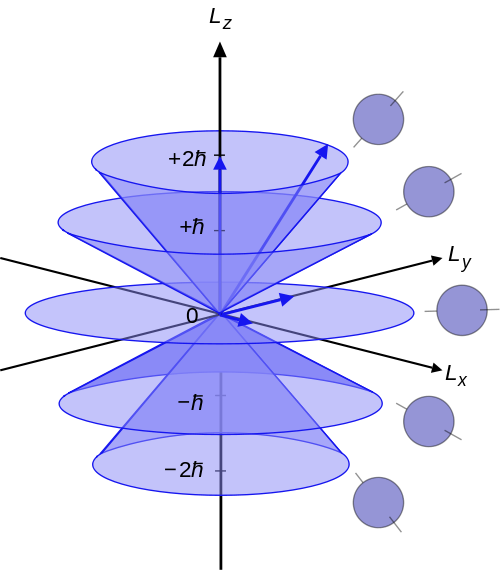
\includegraphics[width=0.5\linewidth]{./img/OEP_wiki2} 

}

\caption{Illustration of the vector model of orbital angular momentum.}\label{fig:Fig1c6}
\end{figure}

\hypertarget{Spin}{%
\chapter{Spin}\label{Spin}}

Spin is a special property of particles that has no classical analogue. Spin is an intrinsic form of angular momentum carried by elementary particles, such as the electron.

\hypertarget{stern-gerlach-experiment}{%
\section{Stern-Gerlach Experiment}\label{stern-gerlach-experiment}}

In 1920, Otto Stern and Walter Gerlach designed an experiment that unintentionally led to the discovery that electrons have their own individual, continuous spin even as they move along their orbital of an atom. The experiment was done by putting a silver foil in an oven to vaporize its atoms. The silver atoms were collected into a beam that passed through an inhomogeneous magnetic field. The result was that the magnetic beam split the beam into two (and only two) separate ones. The Stern--Gerlach experiment demonstrated that the spatial orientation of angular momentum is quantized into two components (up and down). Thus an atomic-scale system was shown to have intrinsically quantum properties. The experiment is normally conducted using electrically neutral particles such as silver atoms. This avoids the large deflection in the path of a charged particle moving through a magnetic field and allows spin-dependent effects to dominate.

If the particle is treated as a classical spinning magnetic dipole, it will precess in a magnetic field because of the torque that the magnetic field exerts on the dipole. If it moves through a homogeneous magnetic field, the forces exerted on opposite ends of the dipole cancel each other out and the trajectory of the particle is unaffected. However, if the magnetic field is inhomogeneous then the force on one end of the dipole will be slightly greater than the opposing force on the other end, so that there is a net force which deflects the particle's trajectory. If the particles were classical spinning objects, one would expect the distribution of their spin angular momentum vectors to be random and continuous. Each particle would be deflected by an amount proportional to its magnetic moment, producing some density distribution on the detector screen. Instead, the particles passing through the Stern--Gerlach apparatus are equally distributed among two possible values, with half of them ending up at an upper spot (``spin up''), and the other half at the lower spot (``spin down''). Since the particles are deflected by a magnetic field, spin is a magnetic property that is associated to some intrinsic form of angular momentum. As we saw in chapter \ref{Operators}, the quantization of the angular momentum gives energy levels that are \((2\ell+1)\)-fold degenerate. Since along the direction of the magnet we observe only two possible eigenvalues for the spin, we conclude the following value for \(s\):

\begin{equation}
2s+1=2 \quad\Rightarrow\quad s=\frac{1}{2}.
\label{eq:spin0}
\end{equation}

The Stern-Gerlach experiment proves that electrons are spin-\(\frac{1}{2}\) particles. These have only two possible spin angular momentum values measured along any axis, \(+\frac {\hbar }{2}\) or \(-\frac {\hbar }{2}\), a purely quantum mechanical phenomenon. Because its value is always the same, it is regarded as an intrinsic property of electrons, and is sometimes known as ``intrinsic angular momentum'' (to distinguish it from orbital angular momentum, which can vary and depends on the presence of other particles).

The act of observing (measuring) the momentum along the \(z\) direction corresponds to the operator \(\hat{S}_z\), which project the value of the total spin operator \(\hat{S}^2\) along the \(z\) axis. The eigenvalues of the projector operator are:

\begin{equation}
\hat{S}_z \phi = \hbar m_s \phi,
\label{eq:spin0b}
\end{equation}

where \(m_s=\left\{-s,+s\right\}=\left\{-\frac{1}{2},+\frac{1}{2}\right\}\) is the spin quantum number along the \(z\) component. The eigenvalues for the total spin operator \(\hat{S}^2\)---similarly to the angular momentum operator \(\hat{L}^2\) seen in eq. \eqref{eq:angmom1b}---are:

\begin{equation}
\hat{S}^2 \phi = \hbar^2 s(s+1) \phi,
\label{eq:spin0c}
\end{equation}

The initial state of the particles in the Stern-Gerlach experiment is given by the following wave function:

\begin{equation}
\phi = c_1\, \phi_{\uparrow} + c_2 \,\phi_{\downarrow},
\label{eq:spin1}
\end{equation}

where \(\uparrow=+\frac{\hbar}{2}\), \(\downarrow=-\frac{\hbar}{2}\), and the coefficients \(c_1\) and \(c_2\) are complex numbers. In this initial state, spin can point in any direction. The expectation value of the operator \(\hat{S}_z\) (the quantity that the Stern-Gerlach experiment measures), can be obtained using eq. \eqref{eq:ee6}:

\begin{equation}
\begin{aligned}
<S_z> &= \int \phi^{*} \hat{S}_z \phi \, d\mathbf{s} \\
 &= +\frac{\hbar}{2} \vert c_1\vert^2 -\frac{\hbar}{2} \vert c_2\vert^2,
\end{aligned}
\label{eq:spin2}    
\end{equation}

where the integration is performed along a special coordinate \(\mathbf{s}\) composed of only two values, and the coefficient \(c_1\) and \(c_2\) are complex numbers. Applying the normalization condition, eq. \eqref{eq:ee4} we can obtain:

\begin{equation}
|c_{1}|^{2}+|c_{2}|^{2}=1 \quad\longrightarrow\quad |c_{1}|^{2}=|c_{2}|^{2}=\frac{1}{2}.
\label{eq:spin3}    
\end{equation}

This equation is not sufficient to determine the values of the coefficients since they are complex numbers. Eq. \eqref{eq:spin3}, however, tells us that the squared magnitudes of the coefficients can be interpreted as probabilities of outcome from the experiment. This is true because their values are obtained from the normalization condition, and the normalization condition guarantees that the system is observed with probability equal to one. Summarizing, since we started with random initial directions, each of the two states, \(\phi_{\uparrow}\) and \(\phi_{\downarrow}\), will be observed with equal probability of \(\frac{1}{2}\).

\hypertarget{sequential-stern-gerlach-experiments}{%
\section{Sequential Stern-Gerlach Experiments}\label{sequential-stern-gerlach-experiments}}

An interesting result can be obtain if we link multiple Stern--Gerlach apparatuses into one experiment and we perform the measurement along two orthogonal directions in space.
As we showed in the previous section, all particles leaving the first Stern-Gerlach apparatus are in an eigenstate of the \(\hat{S}_z\) operator (i.e., their spin is either ``up or''down" with respect to the \(z\)-direction). We can then take either one of the two resulting beams (for simplicity let's take the ``spin up'' output), and perform another spin measurement on it. If the second measurement is also aligned along the \(z\)-direction then only one outcome will be measured, since all particles are already in the ``spin up'' eigenstate of \(\hat{S}_z\). In other words, the measurement of a particle being in an eigenstate of the corresponding operator leaves the state unchanged.

If, however, we perform the spin measurement along a direction perpendicular to the original \(z\)-axis (i.e., the \(x\)-axis) then the output will equally distribute among ``spin up'' or ''spin down'' in the \(x\)-direction, which in order to avoid confusion, we can call ``spin left'' and ``spin right''. Thus, even though we knew the state of the particles beforehand, in this case the measurement resulted in a random spin flip in either of the measurement directions. Mathematically, this property is expressed by the nonvanishing of the commutator of the spin operators:

\begin{equation}
\left[\hat{S}_z,\hat{S}_x \right] \neq 0.
\label{eq:spin4}    
\end{equation}

We can finally repeat the measurement a third time, with the magnet aligned along the original \(z\)-direction. According to classical physics, after the second apparatus, we would expect to have one beam with characteristic ``spin up'' and ``spin left'', and another with characteristic ``spin up'' and ``spin right''. The outcome of the third measurement along the original \(z\)-axis should be one output with characteristic ``spin up'', regardless to which beam the magnet is applied (since the ``spin down'' component should have been ``filtered out'' by the first experiment, and the ``spin left'' and ``spin right'' component should be filtered out by the third magnet). This is not what is observed. The output of the third measurement is---once again---two beams in the \(z\) direction, one with ``spin up'' characteristric and the other with ``spin down''.

This experiment shows that spin is not a classical property. The Stern-Gerlach apparatus does not behave as a simple filter, selecting beams with one specific pre-determined characteristic. The second measurement along the \(x\) axis destroys the previous determination of the angular momentum in the \(z\) direction. This means that this property cannot be measured on two perpendicular directions at the same time.

\hypertarget{spin-operators}{%
\section{Spin Operators}\label{spin-operators}}

The mathematics of quantum mechanics tell us that \(\hat{S}_z\) and \(\hat{S}_x\) do not commute. When two operators do not commute, the two measurable quantities that are associated with them cannot be known at the same time.

In 3-dimensional space there are three directions that are orthogonal to each other \(\left\{x,y,z\right\}\). Thus, we can define a third spin projection operator along the \(y\) direction, \(\hat{S}_y\), corresponding to a new set of Stern-Gerlach experiments where the second magnet is oriented along a direction that is orthogonal to the two that we consider in the previous section. The total spin operator, \(\hat{S}^2\), can then be constructed similarly to the total angular momentum operator of eq. \eqref{eq:angmom1}, as:

\begin{equation}
\begin{aligned}
\hat{S}^2 &=\hat{S}\cdot\hat{S}=\left(\mathbf{i}\hat{S}_x+\mathbf{j}\hat{S}_y+\mathbf{k}\hat{S}_z\right)\cdot\left(\mathbf{i}\hat{S}_x+\mathbf{j}\hat{S}_y+\mathbf{k}\hat{S}_z \right) \\
&=\hat{S}_x^2+\hat{S}_y^2+\hat{S}_z^2,
\end{aligned}
\label{eq:spop1}    
\end{equation}

with \(\left\{\mathbf{i},\mathbf{j},\mathbf{k}\right\}\) the unitary vectors in three-dimensional space.

Wolfgang Pauli explicitly derived the relationships between all three spin projection operators. Assuming the magnetic field along the \(z\) axis, Pauli's relations can be written using simple equations involving the two possible eigenstates \(\phi_{\uparrow}\) and \(\phi_{\downarrow}\):

\begin{equation}
\begin{aligned}
\hat{S}_x \phi_{\uparrow} =  \frac{\hbar}{2} \phi_{\downarrow} \qquad \hat{S}_y \phi_{\uparrow} &=  \frac{\hbar}{2} i \phi_{\downarrow} \qquad \hat{S}_z \phi_{\uparrow} =  \frac{\hbar}{2} \phi_{\uparrow} \\
\hat{S}_x \phi_{\downarrow} =  \frac{\hbar}{2} \phi_{\uparrow} \qquad \hat{S}_y \phi_{\downarrow} &=  - \frac{\hbar}{2} i \phi_{\uparrow} \qquad \hat{S}_z \phi_{\downarrow} =  -\frac{\hbar}{2} \phi_{\downarrow},
\end{aligned}
\label{eq:spop2}  
\end{equation}

where \(i\) is the imaginary unit (\(i^2=-1\)). In other words, for \(\hat{S}_z\) we have eigenvalue equations, while the remaining components have the effect of permuting state \(\phi_{\uparrow}\) with state \(\phi_{\downarrow}\) after multiplication by suitable constants. We can use these equations, together with eq. \eqref{eq:bp5}, to calculate the commutator for each couple of spin projector operators:

\begin{equation}
\begin{aligned}
\left[\hat{S}_x, \hat{S}_y\right] &= i\hat{S}_z \\
\left[\hat{S}_y, \hat{S}_z\right] &= i\hat{S}_x \\
\left[\hat{S}_z, \hat{S}_x\right] &= i\hat{S}_y,
\end{aligned}
\label{eq:spop3}  
\end{equation}

which prove that the three projection operators do not commute with each other.

\begin{quote}
\begin{example}
\protect\hypertarget{exm:spinex1}{}{\label{exm:spinex1} }\emph{Proof of Commutator Between Spin Projection Operators.}

The equations in \eqref{eq:spop3} can be proved by writing the full eigenvalue equation and solving it using the definition of commutator, eq.\eqref{eq:bp5}, in conjunction with Pauli's relation, eqs. \eqref{eq:spop2}. For example, for the first couple:

\begin{equation}
\begin{aligned}
\left[\hat{S}_x, \hat{S}_y\right] \phi_{\uparrow} &= \hat{S}_x\hat{S}_y\phi_{\uparrow}-\hat{S}_y\hat{S}_x\phi_{\uparrow} \\
&= \hat{S}_x \left(\frac{\hbar}{2}i \phi_{\downarrow} \right)-\hat{S}_y \left(\frac{\hbar}{2} \phi_{\downarrow} \right) \\
&= \frac{\hbar}{2}i \left(\frac{\hbar}{2}i \phi_{\downarrow} \right)- \frac{\hbar}{2} \left(\frac{\hbar}{2} \phi_{\downarrow} \right) \\
&= \left(\frac{\hbar}{4}+\frac{\hbar}{4}\right)i\phi_{\uparrow} \\
&= \frac{\hbar}{2}i \phi_{\uparrow} \\
&= i\hat{S}_z  \phi_{\uparrow} 
\end{aligned}
\label{eq:spop4} 
\end{equation}
\end{example}
\end{quote}

\hypertarget{Postulates}{%
\chapter{Postulates of Quantum Mechanics}\label{Postulates}}

In order to understand deeper quantum mechanics, scientists have derived a series of axioms that result in what are called \emph{postulates of quantum mechanics}. These are, in fact, assumptions that we need to make to understand how the measured reality relates with the mathematics of quantum mechanics. It is important to notice that the postulates are necessary for the interpretation of the theory, but not for the mathematics behind it. Regarding of whether we interpret it or not, the mathematics is complete and consistent. In fact, as we will see in the next chapter, several controversies regarding the interpretation of the mathematics are still open, and different philosophies have been developed to rationalize the results. Recall also that there are different ways of writing the equation of quantum mechanics, all equivalent to each other (i.e., Schrödinger's differential formulation and Heisenberg's algebraic formulation that we saw in chapter \ref{Schrodinger}). For these reasons, there is not an agreement on the number of postulates that are necessary to interpret the theory, and some philosophy and/or formulation might require more postulates than others. In this chapter, we will discuss the six postulates, as they are usually presented in chemistry and introductory physics textbooks and as they relate with a basic statistical interpretation of quantum mechanics. Regardless of the philosophical consideration on the meanings and numbers of the postulate, as well as their physical origin, these statements will make the interpretation of the theory a little easier, as we will see in the next chapter.

\hypertarget{postulate-1-the-wave-function-postulate}{%
\section{Postulate 1: The Wave Function Postulate}\label{postulate-1-the-wave-function-postulate}}

The state of a quantum mechanical system is completely specified by a function \(\Psi({\bf r}, t)\) that depends on the coordinates of the particle(s) and on time. This function, called the wave function or state function, has the important property that \(\Psi^{*}({\bf r}, t)\Psi({\bf r}, t) d\tau\) is the probability that the particle lies in the volume element \(d\tau\) located at \({\bf r}\) at time \(t\).

The wave function must satisfy certain mathematical conditions because of this probabilistic interpretation. For the case of a single particle, the probability of finding it somewhere is 1, so that we have the normalization condition

\begin{equation}
\int_{-\infty}^{\infty} \Psi^{*}({\bf r}, t) \Psi({\bf r}, t) d\tau = 1
\label{eq:post1}  
\end{equation}

It is customary to also normalize many-particle wave functions to 1. As we already saw for the particle in a box in chapter \ref{Models}, a consequence of the first postulate is that the wave function must also be single-valued, continuous, and finite, so that derivatives can be defined and calculated at each point in space. This consequence allows for operators (which typically involve derivation) to be applied without mathematical issues.

\hypertarget{postulate-2-experimental-observables}{%
\section{Postulate 2: Experimental Observables}\label{postulate-2-experimental-observables}}

To every observable in classical mechanics there corresponds a linear, Hermitian operator in quantum mechanics. We have in part already discussed this postulate in chapter \ref{Operators}, albeit we didn't call it as such. This postulate is necessary if we require the expectation value of an operator \(\hat{A}\) to be real, as it should be.

\hypertarget{postulate-3-individual-measurements}{%
\section{Postulate 3: Individual Measurements}\label{postulate-3-individual-measurements}}

In any measurement of the observable associated with operator \(\hat{A}\), the only values that will ever be observed are the eigenvalues \(a\) that satisfy the eigenvalue equation:

\begin{equation}
\hat{A} \Psi = a \Psi.
\label{eq:post2}  
\end{equation}

This postulate captures the central point of quantum mechanics: the values of dynamical variables can be quantized (although it is still possible to have a continuum of eigenvalues in the case of unbound states). If the system is in an eigenstate of \(\hat{A}\) with eigenvalue \(a\), then any measurement of the quantity \(A\) will yield \(a\).
Although measurements must always yield an eigenvalue, the state does not have to be an eigenstate of \(\hat{A}\) initially.

An arbitrary state can be expanded in the complete set of eigenvectors of \(\hat{A}\) \(\left(\hat{A}\Psi_i = a_i \Psi_i\right)\) as:

\begin{equation}
\Psi = \sum_i^{n} c_i \Psi_i,
\label{eq:post3}  
\end{equation}

where \(n\) may go to infinity. In this case, we only know that the measurement of \(A\) will yield one of the values \(a_i\), but we don't know which one. However, we do know the probability that eigenvalue \(a_i\) will occur (it is the absolute value squared of the coefficient, \(\vert c_i\vert^2\), as we obtained already in chapter \ref{Operators}), leading to the fourth postulate below.

\hypertarget{postulate-4-expectation-values-and-collapse-of-the-wavefunction}{%
\section{Postulate 4: Expectation Values and Collapse of the Wavefunction}\label{postulate-4-expectation-values-and-collapse-of-the-wavefunction}}

If a system is in a state described by a normalized wave function \(\Psi\), then the average value of the observable corresponding to \(\hat{A}\) is given by:

\begin{equation}
<A> = \int_{-\infty}^{\infty} \Psi^{*} \hat{A} \Psi d\tau.
\label{eq:post4}  
\end{equation}

An important consequence of the fourth postulate is that, after measurement of \(\Psi\) yields some eigenvalue \(a_i\), the wave function immediately ``collapses'' into the corresponding eigenstate \(\Psi_i\). In other words, measurement affects the state of the system. This fact is used in many experimental tests of quantum mechanics, such as the Stern-Gerlach experiment. Think again at the sequential experiment that we discussed in chapter \ref{Spin}. The act of measuring the spin along one coordinate is not simply a ``filtration'' of some pre-existing feature of the wave function, but rather an act that changes the nature of the wave function itself, affecting the outcome of future experiments. To this act corresponds the collapse of the wave function, a process that remains unexplained to date. Notice how the controversy is not in the mathematics of the experiment, which we already discussed in the previous chapter without issues. The issues rather arise because we don't know how to define the measurement act in itself (other than the fact that it is some form of quantum mechanical procedure with clear and well-defined macroscopic outcomes). This is the reason why the collapse of the wave function is also sometimes called the \emph{measurement problem} of quantum mechanics, and it is still a source of research and debate among modern scientists.

\hypertarget{postulate-5-time-evolution}{%
\section{Postulate 5: Time Evolution}\label{postulate-5-time-evolution}}

The wave function of a system evolves in time according to the time-dependent Schrödinger equation:

\begin{equation}
\hat{H} \Psi({\bf r}, t) = i \hbar \frac{\partial \Psi}{\partial t}.
\label{eq:post5}  
\end{equation}

The central equation of quantum mechanics must be accepted as a postulate.

\hypertarget{postulate-6-pauli-exclusion-principle}{%
\section{Postulate 6: Pauli Exclusion Principle}\label{postulate-6-pauli-exclusion-principle}}

The total wave function of a system with \(N\) spin-\(\frac{1}{2}\) particles (also called \textbf{fermions}) must be antisymmetric with respect to the interchange of all coordinates of one particle with those of another. For spin-1 particles (also called \textbf{bosons}), the wave function is symmetric:

\begin{equation}
\begin{aligned}
\Psi\left({\bf r}_1,{\bf r}_2,\ldots, {\bf r}_N\right) &= - \Psi\left({\bf r}_2,{\bf r}_1,\ldots, {\bf r}_N\right) \quad \text{fermions}, \\
\Psi\left({\bf r}_1,{\bf r}_2,\ldots, {\bf r}_N\right) &= + \Psi\left({\bf r}_2,{\bf r}_1,\ldots, {\bf r}_N\right) \quad \text{bosons}.
\end{aligned}
\label{eq:post6}  
\end{equation}

Electronic spin must be included in this set of coordinates. As we will see in chapter \ref{Atoms}, the mathematical treatment of the antisymmetry postulate gives rise to the Pauli exclusion principle, which states that two or more identical fermions cannot occupy the same quantum state simultaneously (while bosons are perfectly capable of doing so).

\hypertarget{Weirdness}{%
\chapter{Quantum Weirdness}\label{Weirdness}}

In this chapter, we will delve deeper into the strangeness of quantum mechanics. In particular, we will explore quantum phenomena that don't have a classical counterpart, starting from perhaps the most simple but also one of the most revealing: the double-slit experiment.

\hypertarget{the-double-slit-experiment}{%
\section{The double-slit experiment}\label{the-double-slit-experiment}}

The double-slit experiment is considered by many the seminal experiment in quantum mechanics. The reason why we see it only at this advanced point is that its interpretation is not as straightforward as it might seem from a superficial analysis. The famous physicist Richard Feynman was so fond of this experiment that he used to say that all of quantum mechanics can be understood from carefully thinking through its implications.

The premises of the experiment are very simple: cut two slits in a solid material (such as a sheet of metal), send light or electrons through them, and observe what happens on a screen position at some distance on the other side. The result of this experiment though are far from straightforward.

Let's first consider the single-slit case. If light consisted of classical particles, and these particles were sent in a straight line through a single-slit and allowed to strike a screen on the other side, we would expect to see a pattern corresponding to the size and shape of the slit. However, when this ``single-slit experiment'' is actually performed, the pattern on the screen is a diffraction pattern in which the light is spread out. The smaller the slit, the greater the angle of spread. This behavior is typical of waves, where diffraction explains the pattern as being the result of the interference of the waves with the slit.

If one illuminates two parallel slits, the light from the two slits again interferes. Here the interference is a more pronounced pattern with a series of alternating light and dark bands. The width of the bands is a property of the frequency of the illuminating light. The pattern observed on the screen is the result of this interference, as shown in figure \ref{fig:Fig1c9}.\footnote{This diagram is taken from \href{https://en.wikipedia.org/wiki/Double-slit_experiment\#/media/File:Single_slit_and_double_slit2.jpg}{Wikipedia} by user Jordgette, and distributed under CC BY-SA 3.0 license.}

\begin{figure}

{\centering 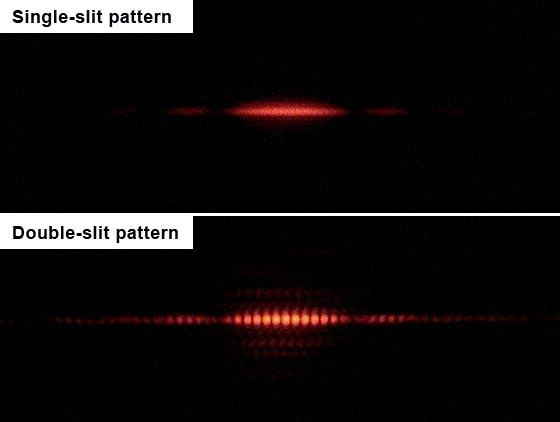
\includegraphics[width=0.7\linewidth]{./img/OEP_wiki3} 

}

\caption{Outcomes of single-slit and double-slit experiments.}\label{fig:Fig1c9}
\end{figure}

The interference pattern resulting from the double-slit experiment are observed not only with light, but also with a beam of electrons, and other small particles.

\hypertarget{the-individual-particles-experiment}{%
\subsection{The individual particles experiment}\label{the-individual-particles-experiment}}

The first twist in the plot is if we perform the experiment by sending individual particles (e.g, either individual photons, or individual electrons). Sending particles through a double-slit apparatus one at a time results in single particles appearing on the screen, as expected. Remarkably, however, an interference pattern emerges when these particles are allowed to build up one by one (figure \ref{fig:Fig2c9}\footnote{This diagram is taken from \href{https://en.wikipedia.org/wiki/Double-slit_experiment\#/media/File:Interference_electrons_double-slit_at_10cm.png}{Wikipedia} by user Alexandre Gondran, and distributed under CC BY-SA 4.0 license}). The resulting pattern on the screen is the same as if each individual particle had passed through both slits.

\begin{figure}

{\centering 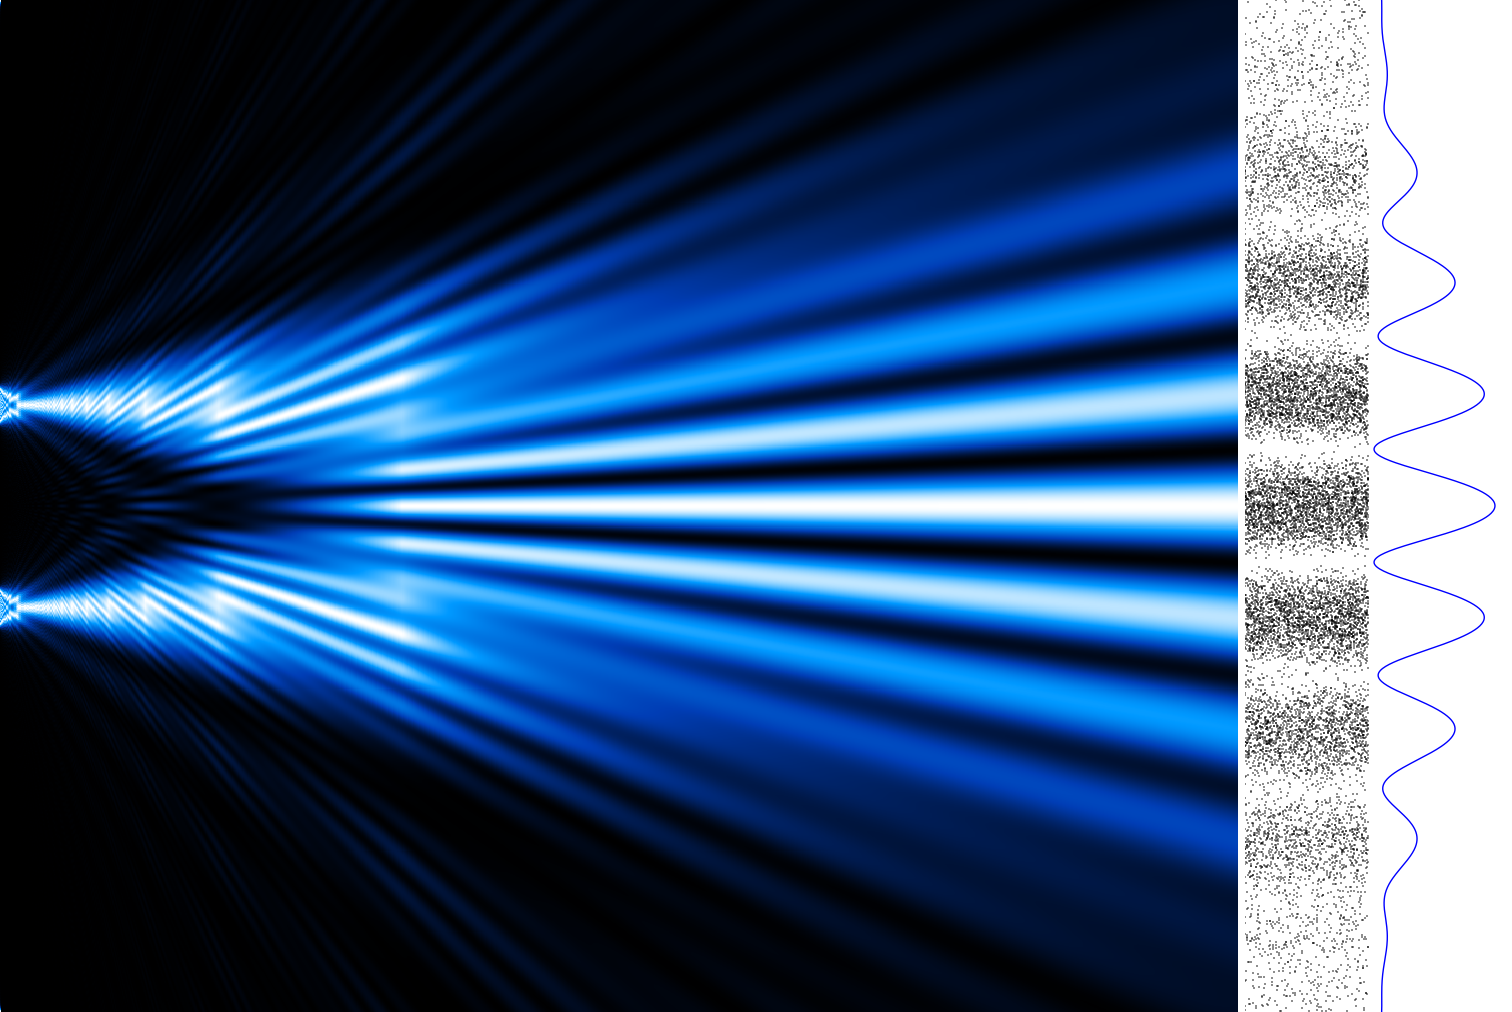
\includegraphics[width=0.7\linewidth]{./img/OEP_wiki4} 

}

\caption{Numerical simulation of the double-slit experiment with electrons.}\label{fig:Fig2c9}
\end{figure}

This variation of the double-slit experiment demonstrates the wave--particle duality: the particle is measured as a single pulse at a single position, while the wave describes the probability of absorbing the particle at a specific place on the screen.

\hypertarget{which-way-experiment}{%
\subsection{``Which way'' experiment}\label{which-way-experiment}}

A second twist happens if we place particle detectors at the slits with the intent of showing through which slit a particle goes. The interference pattern in this case will disappear.

This experiment illustrates that photons (and electrons) can behave as either particles or waves, but cannot be observed as both at the same time. The simplest interpretation of this experiment is that the wave function of the photon collapses into a deterministic position due to the interaction with the detector on the slit, and the interference pattern is therefore lost. This result also proves that in order to measure (detect) a photon, we must interact with it, an act that changes its wave function.

The interpretation of the results of this experiment is not simple. As for other situations in quantum mechanics, the problem arise not because we cannot describe the experiment in mathematical terms, but because the math that we need to describe it cannot be related to the macroscopic classical world we live in. According to the math, in fact, particles in the experiment are described exclusively in probabilistic terms (given by the square of the wave function). The macroscopic world, however, is not probabilistic, and outcomes of experiments can be univocally measured. Several different ways of reediming this controversy have been proposed, including for example the possibility that quantum mechanics is incomplete (the emergence of probability is due to the ignorance of some more fundamental deterministic feature of nature), or assuming that every time a measurement is done on a quantum system, the universe splits, and every possible measurable outcome is observed in different branches of our universe (we only happen to live in one of such branches, so we observe only one non-probabilistic result).\footnote{The interested student can read more about different interpretations \href{https://en.wikipedia.org/wiki/Interpretations_of_quantum_mechanics}{HERE}.} The interpretation of quantum mechanics is still an unsolved problem in modern physics (luckily, it does not prevent us from using quantum mechanics in chemistry).

\hypertarget{heisenbergs-uncertainty-principle}{%
\section{Heisenberg's Uncertainty Principle}\label{heisenbergs-uncertainty-principle}}

Let's now revisit the simple case of a free particle. As we saw in chapter \ref{Models}, the wave function that solved the TISEq:

\begin{equation}
\psi(x) = A \exp(\pm ikx),
\label{eq:heis0}  
\end{equation}

is the equation of a plane wave along the \(x\) direction. This result is in agreement with the de Broglie hypothesis, which says that every object in the universe is a wave. If this wave function describes a particle with mass (such as an electron), freely moving along one spatial direction \(x\), it would be reasonable to ask the question: where is the particle located? Analyzing eq. \eqref{eq:heis0}, however, it is not possible to answer this question since \(\psi(x)\) is delocalized in space from \(x=-\infty\) to \(x=+\infty\).\footnote{The time-dependent picture does not help us either, but since it is a little more complicated to work with the TDSEq, we are not showing it here.} In other words, the particle position is extremely uncertain because it could be essentially anywhere along the wave.

Thus for a free particle, the particle side of the wave-particle duality seems completely lost. We can, however, bring it back into the picture by writing the wave function as a sum of many plane waves, called a \emph{wave packet}:

\begin{equation} 
\psi (x)\propto \sum _{n}A_{n}\exp\left(\frac{ip_n x}{\hbar} \right),
\label{eq:heis1}  
\end{equation}

where \(A_n\) represents the relative contribution of the mode \(p_n\) to the overall total. We are allowed to write the wave function this way because each individual plane wave is a solution of the TISEq, and as we already saw in chapter \ref{Operators} and several other places, the sum of each individual solution is also a solution. An interesting consequence of writing the wave function as a wave packet is that when we sum different waves, they interfere with each other, and they might localize in some region of space. Thus for a wave function written as in eq. \eqref{eq:heis1}, the wave packet can become more localized. We may also make this procedure a step further to the continuum limit, where the wave function goes from a sum to an integral over all possible modes:

\begin{equation}
\psi (x)=\frac {1}{\sqrt{2\pi\hbar}}\int_{-\infty }^{\infty }\varphi (p)\cdot \exp
\left(\frac{ip x}{\hbar} \right)\,dp,
\label{eq:heis2}  
\end{equation}

where \(\varphi(p)\) represents the amplitude of these modes and is called the wave function in momentum space. In mathematical terms, we say that \(\varphi (p)\) is the Fourier transform of \(\psi (x)\) and that \(x\) and \(p\) are conjugate variables. Adding together all of these plane waves comes at a cost; namely, the momentum has become less precise since it becomes a mixture of waves of many different momenta.

One way to quantify the precision of the position and momentum is the standard deviation, \(\sigma\). Since \(|\psi (x)|^{2}\) is a probability density function for position, we calculate its standard deviation. The precision of the position is improved---i.e., reduced \(\sigma_x\)---by using many plane waves, thereby weakening the precision of the momentum---i.e., increased \(\sigma_p\). Another way of stating this is that \(\sigma_x\) and \(\sigma_p\) have an inverse relationship (once we know one with absolute precision, the other becomes completely unknown). This fact was discovered by Werner Heisenberg and is now called the \textbf{Heisenberg's uncertainty principle}. The mathematical treatment of this procedure results in the simple formula:

\begin{equation}
\sigma_{x}\sigma_{p} \geq \frac{\hbar }{2}.
\label{eq:heis3}  
\end{equation}

The uncertainty principle can be extended to any couple of conjugated variables, including, for example, energy and time, angular momentum components along perpendicular directions, spin components along perpendicular directions, etc. It is also easy to show that conjugate variables in quantum mechanics correspond to non-commuting operators.\footnote{Therefore, a simpler way of finding if two variables are subject to the uncertainty principle is to check if their corresponding operators commute.}

\hypertarget{tunneling}{%
\section{Tunneling}\label{tunneling}}

Tunneling is a phenomenon where a particle may cross a barrier even if it does not have sufficient kinetic energy to overcome the potential of the barrier itself. In this situation, the particle is said to ``tunnel through'' the barrier following a purely quantum mechanical phenomenon (figure \ref{fig:Fig3c9}).\footnote{This diagram is taken from \href{https://en.wikipedia.org/wiki/Quantum_tunnelling\#/media/File:TunnelEffektKling1.png}{Wikipedia} by user Felix Kling, and distributed under CC BY-SA 3.0 license.}

\begin{figure}

{\centering 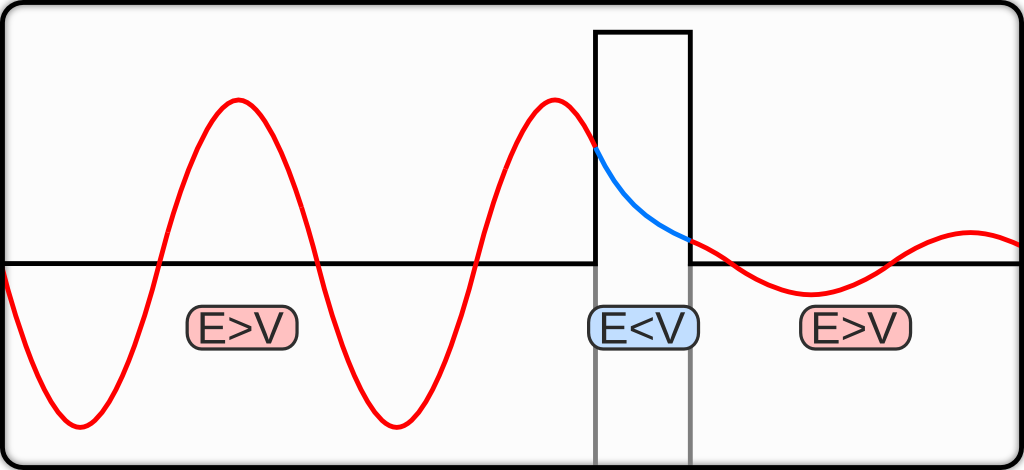
\includegraphics[width=0.7\linewidth]{./img/OEP_wiki9} 

}

\caption{Quantum tunneling through a barrier. The energy of the tunnelled particle is the same but the probability amplitude is decreased.}\label{fig:Fig3c9}
\end{figure}

To explain tunneling we must resort once again to the TISeq. A traveling or standing wave function incident on a non-infinite potential barrier (\(V_0\)) decays in the potential as a function of \(A_0\exp[-\alpha x]\), where \(A_0\) is the amplitude at the boundary, \(\alpha\) is proportional to the potential, and \(x\) is the distance into the potential. If a second well exists at infinite distance from the first well, the probability goes to zero, so the probability of a particle existing in the second well is zero. If a second well is brought closer to the first well, the amplitude of the wave function at this boundary is not zero, so the particle may tunnel into that well from the first well. It would appear that the particle is ``leaking'' through the barrier; it can travel through it without having to surmount it. An important point to keep in mind is that tunneling conserves energy. The final sum of the kinetic and potential energy of the system cannot exceed the initial sum. Therefore, the potential on both sides of the barrier does not need to be the same, but the sum of the ground state energy and the potential on the opposite side of the barrier may not be larger than the initial particle energy and potential.

Tunneling can be described using the TISEq, eq. \eqref{eq:hamilt1}. For the tunneling problem we can take the potential \(V\) to be zero for all space, except for the region inside the barrier (between \(0\) and \(a\)):

\begin{equation}
V=\begin{cases} 0\quad&\text{if}\; -\infty<x\leq 0 \\ V_0\quad&\text{if}\; 0<x<a \\ 0\quad&\text{if}\; a\leq x< \infty \end{cases}.
\label{eq:tunn1}  
\end{equation}

To solve the TISEq with this potential, we must solve it separately for each region, but we should make sure that the wave function stays single-valued, continuous and everywhere continuously differentiable. The general solution for each region, before applying the boundary conditions, is:

\begin{equation}
\psi=\begin{cases} A\sin (kx)+B\cos (kx)\quad&\text{if}\; -\infty<x\leq 0 \\ C \exp(-\alpha x)+D\exp(\alpha x) \quad&\text{if}\; 0<x<a \\ E\sin (kx)+F\cos (kx) \quad&\text{if}\; a\leq x< \infty \end{cases}
\label{eq:tunn2}  
\end{equation}

where \(k=\frac{\sqrt{2mE}}{\hbar}\), and \(\alpha=\frac{\sqrt{2m(V_0-E)}}{\hbar}\). To enforce continuity, we must have at the first boundary:

\begin{equation}
A\sin(0) +B \cos(0)=C\exp(0)+D\exp(0),
\label{eq:tunn3}  
\end{equation}

which implies that \(A=0\), and \(B=C+D\). At the opposite boundary:

\begin{equation}
A\sin(ka) +B \cos(ka)=C\exp(-\alpha a)+D\exp(\alpha a).
\label{eq:tunn4}  
\end{equation}

We notice that, as \(a\) goes to infinity, the right hand side of eq. \eqref{eq:tunn4} goes to infinity, which does not make physical sense. To reconcile this, we must set \(D=0\).

For the final region, \(E\) and \(F\), present a potentially intractable problem. However, if one realizes that the value at the boundary \(a\) is driving the wave in the region \(a\) to infinity, it may also be realized that the wave function could be rewritten as \(C\exp[-\alpha a]\cos[k(x-a)]\), phase shifting the wave function by the value of \(a\),
and setting the amplitude to the boundary value. Summarizing, the wave function is:

\begin{equation}
\psi=\begin{cases} B\cos (kx)\quad&\text{if}\; -\infty<x\leq 0 \\ B \exp(-\alpha x)  \quad&\text{if}\; 0<x<a \\ B\exp(-\alpha a)\cos[k(x-a)] \quad&\text{if}\; a\leq x< \infty. \end{cases}
\label{eq:tunn5}  
\end{equation}

Comparing the wave function on the left of the barrier with the one on its right, we notice how the amplitude is attenuated by the barrier as \(\exp\left(-a\frac{\sqrt{2m(V_0-E)}}{\hbar}\right)\), where \(a\) is the width of the barrier, and \((V_0-E)\) is the difference between the potential energy of the barrier and the current energy of the particle. Since the square of the wave function is the probability distribution, the probability of transmission through a barrier is:

\begin{equation}
\exp\left(-2a\frac{\sqrt{2m(V_0-E)}}{\hbar}\right).
\label{eq:tunn6}  
\end{equation}

As the barrier width or height approaches zero, the probability of a particle tunneling through the barrier becomes one. We can also note that \(k\) is unchanged on the other side of the barrier. This implies that the energy of the particle is exactly the same as it was before it tunneled through the barrier, as stated earlier, the only thing that changes is the quantity of particles going in that direction. The rest is reflected off the barrier, and go back the way it came. On the opposite end, as the barrier width or height approaches infinity, the probability of a particle tunneling through the barrier becomes zero, and the barrier behaves similarly to those that contained the particle in the particle in a box example discussed in chapter \ref{Models}.

\hypertarget{Atoms}{%
\chapter{Many-Electron Atoms}\label{Atoms}}

When two or more electrons are present in a system, the TISEq equation cannot be solved analytically. Thus for the vast majority of chemical applications, we must rely on approximate methods. We will explore some of these approximations in this and further chapter, starting from the many-electron atoms (all atoms other than hydrogen). It is important to stress that because of the nature of approximations, this is still a very active field of scientific research, and improved methods are developed every year.

The electronic Hamiltonian for a many-electron atom can be written as:

\begin{equation}
\hat{H}({\bf r}_1,{\bf r}_2,\ldots,{\bf r}_N)=\sum_{i=1}^N \left(-{\frac {\hbar ^{2}}{2m_e }}\nabla_{i}^{2}-{\frac {Ze^{2}}{4\pi \varepsilon _{0}r_{i}}} \right)+{\frac {e^{2}}{4\pi \epsilon _{0}}}\sum_{i<j}\frac{1}{r_{ij}},
\label{eq:atom1}
\end{equation}

where \(Z\) is the nuclear charge, \(m_e\) and \(e\) are respectively the mass and charge of an electron, \({\bf r}_i\) and \(\nabla_i^2\) are the spatial coordinates and the Laplacian of each electron, \(r_{i}=|{\bf r}_i|\), and \(r_{{ij}}=|{\bf r}_i-{\bf r}_j|\) is the distance between two electrons (all other symbols have been explained in previous chapters). The TISEq is easily written using eq. \eqref{eq:scheqsimple}.

\hypertarget{many-electron-wave-functions}{%
\section{Many-Electron Wave Functions}\label{many-electron-wave-functions}}

When we have more than one electron, the sixth postulate that we discussed in chapter \ref{Postulates} comes into place. In other words, we need to account for the spin of the electrons and we need the wave function to be antisymmetric with respect to exchange of the coordinates of any two electrons. In order to do so, we can define a new variable \({\bf x}\) which represents the set of all four coordinates associated with an electron: three spatial coordinates \({\bf r}\), and one spin coordinate \(\mathbf{s}\), i.e., \({\bf x} = \{ {\bf r}, {\bf s} \}\). We can then write the electronic wave function as \(\Psi({\bf x}_1, {\bf x}_2, \ldots, {\bf x}_N)\), and we require the sixth postulate to hold by writing:

\begin{equation}
\Psi\left({\bf x}_1,{\bf x}_2,\ldots, {\bf x}_N\right) = - \Psi\left({\bf x}_2,{\bf x}_1,\ldots, {\bf x}_N\right)
\label{eq:atom2}  
\end{equation}

A very important step in simplifying \(\Psi({\bf x})\) is to expand it in terms of a set of one-electron functions. Since we need to take into account the spin coordinate as well, we can defina a new function, called \textbf{spin-orbital}, by multiplying a spatial orbital by one of the two spin functions:

\begin{equation}
\begin{aligned}
\chi({\bf x}) &= \psi({\bf r}) \phi_{\uparrow}({\bf s}), \\
\chi({\bf x}) &= \psi({\bf r}) \phi_{\downarrow}({\bf s}).
\end{aligned}
\label{eq:atom3}
\end{equation}

Notice that for a given spatial orbital \(\psi({\bf r})\), we can form two spin orbitals, one with \(\uparrow\) spin, and one with \(\downarrow\) spin (since the spin coordinate \({\bf s}\) has only two possible values, as already discussed in chapter \ref{Spin}). For the spatial orbitals we can use the same one-particle functions that solve the TISEq for the hydrogen atom, \(\psi_{n\ell m_{\ell}}({\bf r})\)(eq. \eqref{eq:HA6} in chapter \ref{Hydrogen}). Notice how each spin-orbital now depends on four quantum numbers, the three for the spatial part, \(n,\ell,m_{\ell}\), plus the spin quantum number \(m_s\). We need to keep in mind, however, that the spin-orbitals, \(\chi_{n\ell m_{\ell} m_{s}}\), \emph{are not} analytic solutions to the TISEq, so the resulting wave function is \emph{not} the exact wave function of the system, but just an approximation.

Once we have defined one-electron spin-orbitals for each electron in the system, we can use them as the basis for our many-electron wave function. While doing so, we need to make sure to enforce the antisymmetry property of the overall wave function. We will start from the simplest case of an atom with two electrons with coordinates \(\mathbf{x}_1\) and \(\mathbf{x}_2\), which we put in two spin-orbitals \(\chi_1\) and \(chi_2\). We can write the total wave function as a linear combination of the two spin-orbitals as:

\begin{equation}
\begin{aligned}
\Psi({\bf x}_1, {\bf x}_2) =& b_{11} \chi_1({\bf x}_1) \chi_1({\bf x}_2) + b_{12} \chi_1({\bf x}_1) \chi_2({\bf x}_2) + \\
& b_{21} \chi_2({\bf x}_1) \chi_1({\bf x}_2) + b_{22} \chi_2({\bf x}_1) \chi_2({\bf x}_2).
\end{aligned}
\label{eq:atom4}
\end{equation}

We then notice that in order for the antisymmetry principle to be obeyed, we need \(b_{12} = -b_{21}\) and \(b_{11} = b_{22} = 0\), which give:

\begin{equation}
\Psi({\bf x}_1, {\bf x}_2) = b_{12} \left[ \chi_1({\bf x}_1) \chi_2({\bf x}_2) - \chi_2({\bf x}_1) \chi_1({\bf x}_2)\right].
\label{eq:atom5}
\end{equation}

This wave function is sufficient to describe two-electron atoms and ions, such as helium. The numerical coefficient can be determined imposing the normalization condition, and is equal to \(b_{12} = \frac{1}{\sqrt{2}}\). For the ground state of helium, we can replace the spatial component of each spin-orbital with the \(1s\) hydrogenic orbital, \(\psi_{100}\), resulting in:

\begin{equation}
\begin{aligned}
\Psi({\bf x}_1, {\bf x}_2) &= \frac{1}{\sqrt{2}} \left[ \psi_{100}({\bf r}_1)\phi_{\uparrow} \; \psi_{100}({\bf r}_2)\phi_{\downarrow} - \psi_{100}({\bf r}_1)\phi_{\downarrow} \; \psi_{100}({\bf r}_2)\phi_{\uparrow} \right] \\
&= \psi_{100}({\bf r}_1)\psi_{100}({\bf r}_2) \frac{1}{\sqrt{2}} \left[ \phi_{\uparrow}\phi_{\downarrow} - \phi_{\downarrow}\phi_{\uparrow} \right],
\end{aligned}
\label{eq:atom6}
\end{equation}

which clearly shows how we need just one spatial orbital, \(\psi_{100}\), to describe the system, while the antisymmetry is taken care by a suitable combination of spin functions, \(\frac{1}{\sqrt{2}} \left[ \phi_{\uparrow}\phi_{\downarrow} - \phi_{\downarrow}\phi_{\uparrow} \right]\). Notice also that we commit a small inaccuracy when we say: ``two electron occupies one spin-orbital, one electron has spin up, and the other electron has spin down, with configuration: \([\uparrow\downarrow]\)'', as is typically found in general chemistry textbooks. The reality of the spin configuration is indeed more complicated, and the ground state of helium should be represented as \(\frac{1}{\sqrt{2}}\left[\uparrow\downarrow-\downarrow\uparrow\right]\).

In order to generalize from two electrons to \(N\), we can first observe how eq. \eqref{eq:atom5} could be easily constructed by placing the spin-orbitals into a \(2\times2\) matrix and calculating its determinant:

\begin{equation}
\Psi({\bf x}_1, {\bf x}_2)= \frac{1}{\sqrt{2}}{\begin{vmatrix} \chi_1({\bf x}_1)&\chi_2({\bf x}_1)\\\chi_1({\bf x}_2)&\chi_2({\bf x}_2)
\end{vmatrix}},
\label{eq:atom7}
\end{equation}

where each column contains one spin-orbital, each row contains the coordinates of a single electron, and the vertical bars around the matrix mean that we need to calculate its determinant. This notation is called the \textbf{Slater determinant}, and it is the preferred way of building any \(N\)-electron wave function. Slater determinants are useful because they can be easily bult for any case of \(N\) electrons in \(N\) spin-orbitals, and they also automatically enforce the antisymmetry of the resulting wave function. A general Slater determinant is written:

\begin{equation}
\Psi (\mathbf{x} _{1},\mathbf{x} _{2},\ldots ,\mathbf{x} _{N})={\frac {1}{\sqrt {N!}}}{\begin{vmatrix}\chi _{1}(\mathbf{x} _{1})&\chi _{2}(\mathbf{x} _{1})&\cdots &\chi _{N}(\mathbf{x} _{1})\\\chi _{1}(\mathbf{x} _{2})&\chi _{2}(\mathbf{x} _{2})&\cdots &\chi _{N}(\mathbf{x} _{2})\\\vdots &\vdots &\ddots &\vdots \\\chi _{1}(\mathbf{x} _{N})&\chi _{2}(\mathbf{x} _{N})&\cdots &\chi _{N}(\mathbf{x} _{N})\end{vmatrix}} = |\chi _{1},\chi _{2},\cdots ,\chi _{N}\rangle,
\label{eq:atom8}
\end{equation}

where the notation \(|\cdots\rangle\) is a shorthand to indicate the Slater determinant where only the diagonal elements are reported.

\hypertarget{approximated-hamiltonians}{%
\section{Approximated Hamiltonians}\label{approximated-hamiltonians}}

In order to solve the TISEq for a many-electron atom we also need to approximate the Hamiltonian, since analytic solution using the full Hamiltonian as in eq. \eqref{eq:atom1} are impossible to find. The most significant approximation used in chemistry is called the \emph{variational method}.

\hypertarget{variational-method}{%
\subsection{Variational method}\label{variational-method}}

The basic idea of the variational method is to guess a ``trial'' wave function for the problem consisting of some adjustable parameters called ``variational parameters''. These parameters are adjusted until the energy of the trial wave function is minimized. The resulting trial wave function and its corresponding energy are variational method approximations to the exact wave function and energy.

Why would it make sense that the best approximate trial wave function is the one with the lowest energy? This results from the Variational Theorem, which states that the energy of any trial wave function \(E\) is always an upper bound to the exact ground state energy \({\cal E}_0\). This can be proven easily. Let the trial wave function be denoted \(\Phi\). Any trial function can formally be expanded as a linear combination of the exact eigenfunctions \(\Psi_i\). Of course, in practice, we don't know the \(\Psi_i\), since we are applying the variational method to a problem we can't solve analytically. Nevertheless, that doesn't prevent us from using the exact eigenfunctions in our proof, since they certainly exist and form a complete set, even if we don't happen to know them. So, the trial wave function can be written:

\begin{equation}
\Phi = \sum_i c_i \Psi_i,
\label{eq:var1}
\end{equation}

and the approximate energy corresponding to this wave function is:

\begin{equation}
E[\Phi] = \frac{\int \Phi^* {\hat H} \Phi d\mathbf{\tau}}{\int \Phi^* \Phi d\mathbf{\tau}},
\label{eq:var2}
\end{equation}

where \(\mathbf{\tau}=\left(\mathbf{r}_1,\mathbf{r}_2,\ldots,\mathbf{r}_N\right)\) is the ensemble of the spatial coordinates of each electron and the integral symbol is assumed as a \(3N\)-dimensional integration. Replacing the expansion over the exact wave functions, we obtain:

\begin{equation}
E[\Phi] = \frac{\sum_{ij} c_i^* c_j \int \Psi_i^* {\hat H} \Psi_jd\mathbf{\tau}}{
\sum_{ij} c_i^* c_j \int \Psi_i^* \Psi_jd\mathbf{\tau}}.
\label{eq:var3}
\end{equation}

Since the functions \(\Psi_j\) are the exact eigenfunctions of \({\hat H}\), we can use \({\hat H} \Psi_j = {\cal E}_j \Psi_j\) to obtain:

\begin{equation}
E[\Phi] = \frac{\sum_{ij} c_i^* c_j {\cal E}_j \int \Psi_i^* \Psi_j d\mathbf{\tau}}{
\sum_{ij} c_i^* c_j \int \Psi_i^* \Psi_j d\mathbf{\tau}}.
\label{eq:var4}
\end{equation}

Now using the fact that eigenfunctions of a Hermitian operator form an orthonormal set (or can be made to do so), we can write:

\begin{equation}
E[\Phi] = \frac{\sum_{i} c_i^* c_i {\cal E}_i}{\sum_{i} c_i^* c_i}.
\label{eq:var5}
\end{equation}

We now subtract the exact ground state energy \({\cal E}_0\) from both sides to obtain

\begin{equation}
E[\Phi] - {\cal E}_0 = \frac{\sum_i c_i^* c_i ( {\cal E}_i - {\cal E}_0)}{
\sum_i c_i^* c_i}.
\label{eq:var6}
\end{equation}

Since every term on the right-hand side is greater than or equal to zero, the left-hand side must also be greater than or equal to zero:

\begin{equation}
E[\Phi] \geq {\cal E}_0.
\label{eq:varprinciple}
\end{equation}

In other words, the energy of any approximate wave function is always greater than or equal to the exact ground state energy \({\cal E}_0\).

This explains the strategy of the variational method: since the energy of any approximate trial function is always above the true energy, then any variations in the trial function which lower its energy are necessarily making the approximate energy closer to the exact answer. (The trial wave function is also a better approximation to the true ground state wave function as the energy is lowered, although not necessarily in every possible sense unless the limit \(\Phi = \Psi_0\) is reached).

\hypertarget{approximated-solution-for-the-helium-atom}{%
\subsection{Approximated solution for the helium atom}\label{approximated-solution-for-the-helium-atom}}

We now have all the ingredients to attempt the simplest approximated solution to the TISEq of a many-electron atom. We can start by writing the total wave function using the Slater determinant of eq. \eqref{eq:atom8} in terms of spin-orbitals:

\begin{equation}
\Psi (\mathbf{x}_{1},\mathbf{x}_{2},\ldots ,\mathbf{x}_{N})= |\chi_{1},\chi_{2},\cdots ,\chi_{N}\rangle = |\psi_{1}\phi_{\uparrow},\psi_{1}\phi_{\downarrow},\cdots ,\psi_{\frac{N}{2}}\phi_{\uparrow},\psi_{\frac{N}{2}}\phi_{\downarrow}\rangle,
\label{eq:hf1}
\end{equation}

and then we can replace it into the TISEq for an \(N\)-electron system. This results into a set of \(N\) one-electron equations, one for each electron. When we attempt to solve each individual equation, however, we end up with a problem, since the potential energy in the Hamiltonian of eq. \eqref{eq:atom1} does not have spherical symmetry because of the electron-electron repulsion term. As such, the one-electron TISEq cannot be simply solved in spherical polar coordinates, as we did for the hydrogen atom in chapter \ref{Hydrogen}. The simplest way of circumventing the problem is to neglect the electron-electron repulsion term (i.e., assume that the electrons are not correlated and do not interact with each other). For a 2-electron atom this procedure is straightforward, since the Hamiltonian can be written as a sum of one-electron Hamiltonians:

\begin{equation}
\hat{H} =\hat{H}_1+\hat{H}_2,
\label{eq:hf2}
\end{equation}

with \(\hat{H}_1\) and \(\hat{H}_2\) looking identical to those used in the TISEq of the hydrogen atom. This one-particle Hamiltonian does not depend on the spin of the electron, and therefore, we can neglect the spin component of the Slater determinant and write the total wave function for the ground state of helium, eq. \eqref{eq:atom5}, simply as:

\begin{equation}
\Psi({\bf r}_1, {\bf r}_2) = \psi_{100}({\bf r}_1)\psi_{100}({\bf r}_2).
\label{eq:hf3}
\end{equation}

The overall TISEq reduces to a set of two single-particle equations:

\begin{equation}
\begin{aligned}
\hat{H}_1 \psi_{100}({\bf r}_1) &= E_1\psi_{100}({\bf r}_1) \\
\hat{H}_2 \psi_{100}({\bf r}_2) &= E_2\psi_{100}({\bf r}_2),
\end{aligned}
\label{eq:hf4}
\end{equation}

which can then be solved similarly to those for the hydrogen atom, and the solution be combined to give:

\begin{equation}
E = E_1+E_2.
\label{eq:hf5}
\end{equation}

In other words, the resulting energy eigenvalue for the ground state of the helium atom in this approximation is equal to twice the energy of a \(\psi_{100}\), \(1s\), orbital. The resulting approximated value for the energy of the helium atom is \(7,217 \text{ kJ/mol}\), compared with the exact value of \(7,620 \text{ kJ/mol}\).

The nuclear charge \(Z\) in the \(\psi_{100}\) orbital can be used as a variational parameter in the variational method to obtain a more accurate value of the energy. This method provides a result for the ground-state energy of the helium atom of \(7,478 \text{ kJ/mol}\) (only \(142 \text{ kJ/mol}\) lower than the exact value), with the nuclear charge parameter minimized at \(Z_{\text{min}}=1.6875\). This new value of the nuclear charge can be interpreted as the effective nuclear charge that is felt by one electron when a second electron is present in the atom. This value is lower than the real nuclear charge (\(Z=2\)) because the interaction between the electron and the nuclei is shielded by presence of the second electron.

This procedure can be extended to atoms with more than two electrons, resulting in the so-called Hartree-Fock method. The procedure, however, is not straightforward. We will explain it in more details in the next chapter, since it is the simplest approximation that also describes the chemical bond.

\hypertarget{Molecules}{%
\chapter{Molecules}\label{Molecules}}

\hypertarget{the-molecular-hamiltonian}{%
\section{The Molecular Hamiltonian}\label{the-molecular-hamiltonian}}

For a molecule, we can decompose the Hamiltonian operator as:

\begin{equation}
\hat{H} = \hat{K}_N +\hat{K}_{e} + \hat{V}_{NN} + \hat{V}_{eN} + \hat{K}_{ee}
\label{eq:molham1}
\end{equation}

where we have decomposed the kinetic energy operator into nuclear and electronic terms, \(\hat{K}_N\) and \(\hat{K}_e\), as well as the potential energy operator into terms representing the interactions between nuclei, \(\hat{V}_{NN}\), between electrons, \(\hat{V}_{ee}\), and between electrons and nuclei, \(\hat{V}_{eN}\). Each term can then be calculated using:

\begin{equation}
\begin{aligned}
\hat{K}_{N} &=-\sum_{i}^{\text{nuclei}}{\frac  {\hbar ^{2}}{2M_{i}}}\nabla_{{{\mathbf  {R}}_{i}}}^{2} \\
\hat  {K}_{e} &=-\sum_{i}^{\text{electrons}}{\frac  {\hbar ^{2}}{2m_{e}}}\nabla _{{{\mathbf{r}}_{i}}}^{2} \\
\hat{V}_{{NN}} &= \sum _{i}\sum _{{j>i}}{\frac  {Z_{i}Z_{j}e^{2}}{4\pi \varepsilon _{0}\left|{\mathbf  {R}}_{i}-{\mathbf  {R}}_{j}\right|}} \\
\hat  {V}_{{eN}} &=-\sum _{i}\sum _{j}{\frac  {Z_{i}e^{2}}{4\pi \varepsilon_{0}\left|{\mathbf  {R}}_{i}-{\mathbf  {r}}_{j}\right|}} \\
\hat{V}_{{ee}} &= \sum _{i}\sum _{{i<j}}{\frac  {e^{2}}{4\pi \varepsilon _{0}\left|{\mathbf  {r}}_{i}-{\mathbf  {r}}_{j}\right|}},
\end{aligned}
\label{eq:molham2}
\end{equation}

where \(M_i\), \(Z_i\), and \(\mathbf{R}_i\) are the mass, atomic number, and coordinates of nucleus \(i\), respectively, and all other symbols are the same as those used in eq. \eqref{eq:atom1} for the many-electron atom Hamiltonian.

\hypertarget{small-terms-in-the-molecular-hamiltonian}{%
\subsection{Small terms in the molecular Hamiltonian}\label{small-terms-in-the-molecular-hamiltonian}}

The operator in eq. \eqref{eq:molham1} is known as the ``exact'' nonrelativistic Hamiltonian in field-free space. However, it is important to remember that it neglects at least two effects. Firstly, although the speed of an electron in a hydrogen atom is less than 1\% of the speed of light, relativistic mass corrections can become appreciable for the inner electrons of heavier atoms. Secondly, we have neglected the spin-orbit effects, which is explained as follows. From the point of view of an electron, it is being orbited by a nucleus which produces a magnetic field (proportional to \({\bf L}\)); this field interacts with the electron's magnetic moment (proportional to \({\bf S}\)), giving rise to a spin-orbit interaction (proportional to \({\bf L} \cdot {\bf S}\) for a diatomic.) Although spin-orbit effects can be important, they are generally neglected in quantum chemical calculations, and we will neglect them in the remainder of this textbook as well.

\hypertarget{the-born-oppenheimer-approximation}{%
\section{The Born-Oppenheimer Approximation}\label{the-born-oppenheimer-approximation}}

As we already saw in the previous chapter, if a Hamiltonian is separable into two or more terms, then the total eigenfunctions are products of the individual eigenfunctions of the separated Hamiltonian terms. The total eigenvalues are then sums of individual eigenvalues of the separated Hamiltonian terms.

For example. let's consider a Hamiltonian that is separable into two terms, one involving coordinate \(q_1\) and the other involving coordinate \(q_2\):

\begin{equation}
\hat{H} = \hat{H}_1(q_1) + \hat{H}_2(q_2)
\label{eq:molham3}
\end{equation}

with the overall Schrödinger equation being:

\begin{equation}
\hat{H} \psi(q_1, q_2) = E \psi(q_1, q_2).
\label{eq:molham4}
\end{equation}

If we assume that the total wave function can be written in the form:

\begin{equation}
\psi(q_1, q_2) = \psi_1(q_1) \psi_2(q_2),
\label{eq:molham5}
\end{equation}

where \(\psi_1(q_1)\) and \(\psi_2(q_2)\) are eigenfunctions of \(\hat{H}_1\) and \(\hat{H}_2\) with eigenvalues \(E_1\) and \(E_2\), then:

\begin{equation}
\begin{aligned}
\displaystyle \hat{H} \psi(q_1, q_2) &= ( \hat{H}_1 + \hat{H}_2 ) \psi_1(q_1) \psi_2(q_2) \\
 	&= \hat{H}_1 \psi_1(q_1) \psi_2(q_2) + \hat{H}_2 \psi_1(q_1) \psi_2(q_2) \\
 	&= E_1 \psi_1(q_1) \psi_2(q_2) + E_2 \psi_1(q_1) \psi_2(q_2) \\
 	&= (E_1 + E_2) \psi_1(q_1) \psi_2(q_2) \\
 	&= E \psi(q_1, q_2)
\end{aligned}
\label{eq:molham6}
\end{equation}

Thus the eigenfunctions of \(\hat{H}\) are products of the eigenfunctions of \(\hat{H}_1\) and \(\hat{H}_2\), and the eigenvalues are the sums of eigenvalues of \(\hat{H}_1\) and \(\hat{H}_2\).

If we examine the nonrelativistic Hamiltonian in eq. \eqref{eq:molham1}, we see that the \(\hat{V}_{en}\) terms prevents us from cleanly separating the electronic and nuclear coordinates and writing the total wave function. If we neglect these terms, we can write the total wave function as:

\begin{equation}
\psi({\bf r}, {\bf R}) = \psi_e({\bf r}) \psi_N({\bf R}),
\label{eq:molham7}
\end{equation}

This approximation is called the \textbf{Born-Oppenheimer approximation}, and allows us to treat the nuclei as nearly fixed with respect to electron motion. The Born-Oppenheimer approximation is almost always quantitatively correct, since the nuclei are much heavier than the electrons and the (fast) motion of the latter does not affect the (slow) motion of the former. Using this approximation, we can fix the nuclear configuration at some value, \({\bf R_a}\), and solve for the electronic portion of the the wave function, which is dependent only parametrically on \({\bf R}\) (we write this wave function as \(\psi_e \left({\bf r}; {\bf R_a} \right)\), where the semicolon indicate the parametric dependence on the nuclear configuration). To solve the TISEq we can then write the electronic Hamiltonian as:

\begin{equation}
\hat{H}_{\text{e}} = \hat{K}_e({\bf r}) +
\hat{V}_{eN}\left({\bf r}; {\bf R_a} \right) +
\hat{V}_{ee}({\bf r})
\label{eq:molham8}
\end{equation}

where we have also factored out the nuclear kinetic energy, \(\hat{K}_N\) (since it is smaller than \(\hat{K}_e\) by a factor of \(\frac{M_i}{m_e}\)), as well as \(\hat{V}_{NN}({\bf R})\). This latter approximation is justified, since in the Born-Oppenheimer approximation \({\bf R}\) is just a parameter, and \(\hat{V}_{NN}({\bf R_a})\) is a constant that shifts the eigenvalues only by some fixed amount. This electronic Hamiltonian results in the following TISEq:

\begin{equation}
\hat{H}_{e} \psi_e \left({\bf r}; {\bf R_a} \right) = E_{e} \psi_e \left({\bf r}; {\bf R_a} \right),
\label{eq:molham9}
\end{equation}

which is the equation that is used to explain the chemical bond in the next section. Notice that eq. \eqref{eq:molham9} is not the total TISEq of the system, since the nuclear eigenfunction and its eigenvalues (which can be obtained solving the Schrödinger equation with the nuclear Hamiltonian) are neglected.
As a final note, in the remainder of this textbook we will confuse the term ``total energy'' with ``total energy at fixed geometry'', as is customary in many other quantum chemistry textbooks (i.e., we are neglecting the nuclear kinetic energy). This is just \(E_{e}\) of eq. \eqref{eq:molham9}, plus the constant shift,\(\hat{V}_{NN}({\bf R_a})\), given by the nuclear-nuclear repulsion.

\hypertarget{solving-the-electronic-eigenvalue-problem}{%
\section{Solving the Electronic Eigenvalue Problem}\label{solving-the-electronic-eigenvalue-problem}}

Once we have invoked the Born-Oppenheimer approximation, we can attempt to solve the electronic TISEq in eq. \eqref{eq:molham9}. However, for molecules with more than one electron, we need to---once again---keep in mind the antisymmetry of the wave function. This obviously means that we need to write the electronic wave function as a Slater determinant (i.e., all molecules but \(\mathrm{H}_2^+\) and a few related highly exotic ions). Once this is done, we can work on approximating the Hamiltonian, a task that is necessary because the presence of the electron-electron repulsion term forbids its analytic treatment. Similarly to the many-electron atom case, the simplest approximation to solve the molecular electronic TISEq is to use the variational method and to neglect the electron-electron repulsion. As we noticed in the previous chapter, this approximation is called the Hartree-Fock method.

\hypertarget{the-hartree-fock-method}{%
\subsection{The Hartree-Fock Method}\label{the-hartree-fock-method}}

The main difference when we apply the variational principle to a molecular Slater determinant is that we need to build orbitals (one-electron wave functions) that encompass the entire molecule. This can be done by assuming that the atomic contributions to the molecular orbitals will closely resemble the orbitals that we obtained for the hydrogen atom. The total molecular orbital can then be built by linearly combine these atomic contribution. This method is called \textbf{linear combination of atomic orbitals (LCAO)}. A consequence of the LCAO method is that the atomic orbitals on two different atomic centers are not necessarily orthogonal, and eq. \eqref{eq:var4} cannot be simplified easily. If we replace each atomic orbital \(\psi(\mathbf{r})\) with a linear combination of suitable basis functions \(f_i(\mathbf{r})\):

\begin{equation}
\psi(\mathbf{r}) = \sum_i^m c_{i} f_i(\mathbf{r}),
\label{eq:molham10}
\end{equation}

we can then use the following notation:

\begin{equation}
\displaystyle H_{ij} = \int \phi_i^* {\hat H} \phi_j d\mathbf{\tau}\;, \qquad \displaystyle S_{ij} = \int \phi_i^* \phi_jd\mathbf{\tau},
\label{eq:molham11}
\end{equation}

to simplify eq. \eqref{eq:var4} to:

\begin{equation}
E[\Phi] = \frac{\sum_{ij} c_i^* c_j H_{ij}}{\sum_{ij} c_i^* c_j S_{ij}}.
\label{eq:molham11b}
\end{equation}

Differentiating this energy with respect to the expansion coefficients \(c_i\) yields a non-trivial solution only if the following ``secular determinant'' equals zero:

\begin{equation}
\begin{vmatrix}
H_{11}-ES_{11}   & H_{12}-ES_{12}   & \cdots & H_{1m}-ES_{1m}\\\
H_{21}-ES_{21}   & H_{22}-ES_{22}   & \cdots & H_{2m}-ES_{2m}\\\
\vdots           &   \vdots         & \ddots & \vdots\\\
H_{m1}-ES_{m1}   & H_{m2}-ES_{m2}   & \cdots & H_{mm}-ES_{mm}
\end{vmatrix}=0
\label{eq:molham12}
\end{equation}

where \(m\) is the number of basis functions used to expand the atomic orbitals. Solving this set of equations with a Hamiltonian where the electron-electron correlation is neglected results is non-trivial, but possible. The reason for the complications comes from the fact that even if we are neglecting the direct interaction between electrons, each of them interact with the nuclei through an interaction that is screened by the average field of all other electrons, similarly to what we saw for the helium atom. This means that the Hamiltonian itself and the value of the coefficients \(c_i\) in the wave function mutually depend on each other. A solution to this problem can be achieved numerically using specialized computer programs that use a cycle called the \textbf{self-consistent-field (SCF) procedure}. Starting from an initial guess of the coefficients, an approximated Hamiltonian operator is built from them and used to solve eq. \eqref{eq:molham12}. This solution gives updated values of the coefficients, which can then be used to created an improved version of the approximated Hamiltonian. This procedure is repeated until both the coefficients and the operator do not change anymore. From this final solution, the energy of the molecule is then calculated.

\hypertarget{Bonds}{%
\chapter{The Chemical Bond}\label{Bonds}}

In this chapter we will see a couple of examples of how the concept and mathematics of quantum mechanics can be applied to understand the chemical bond in molecules. We will start from the simplest molecule, the \(\mathrm{H}_2^+\) molecular ion, and then we will move on to the simplest two-electron bond in the hydrogen molecule. To simplify the notation in this chapter, we will move away from S.I. units and use a set tailored for molecules, called \emph{atomic units (a.u.)}. This set of units is built by setting \(\hbar=e=m_e=a_0=1\). As an example of the simplification that a.u. allows, the energy eigenvalues of the hydrogen atom, eq. \eqref{eq:HA7}, simply becomes \(E_n=-\frac{1}{2n^2}\) in the a.u. of energy, which are called Hartrees.

\hypertarget{the-chemical-bnd-in-the-hydrogen-molecular-cation}{%
\section{The Chemical Bnd in the Hydrogen Molecular Cation}\label{the-chemical-bnd-in-the-hydrogen-molecular-cation}}

This system has only one electron, but since its geometry is not spherical (figure \ref{fig:Fig1c12}), the TISEq cannot be solved analytically as for the hydrogen atom.

\begin{figure}

{\centering 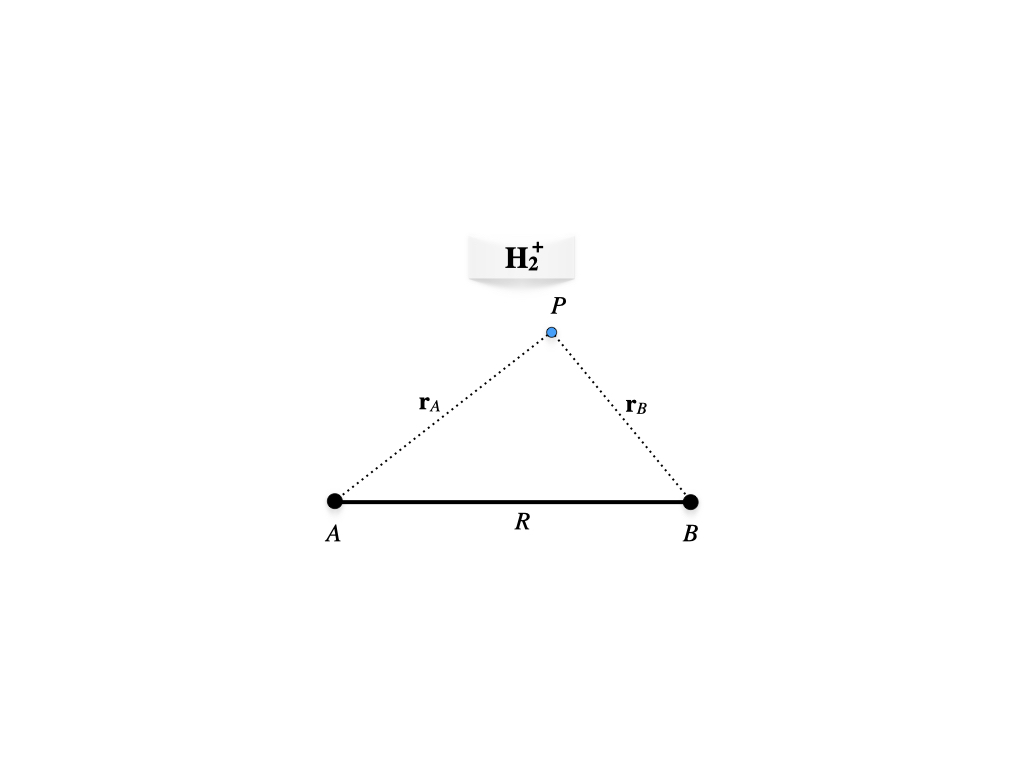
\includegraphics[width=0.7\linewidth]{./img/OEP_figure1} 

}

\caption{Geometry of the hydrogen molecular cation.}\label{fig:Fig1c12}
\end{figure}

The electron is at point \(P\), while the two protons are at position \(A\) and \(B\) at a fixed distance \(R\). Using the Born-Oppenheimer approximation we can write the one-electron molecular Hamiltonian in a.u. as:

\begin{equation}
\hat{H} = \hat{H}_e+\frac{1}{R} = \left( -\frac{1}{2}\nabla^2-\frac{1}{\mathbf{r}_A}-\frac{1}{\mathbf{r}_B} \right)+\frac{1}{R}
\label{eq:bond1}
\end{equation}

As a first approximation to the variational wave function, we can build the one-electron molecular orbital (MO) by linearly combine two \(1s\) hydrogenic orbitals centered at \(A\) and \(B\), respectively:

\begin{equation}
\varphi = c_1 a + c_2 b,
\label{eq:bond2}
\end{equation}

with:

\begin{equation}
\begin{aligned}
a &= 1s_A = \left( \psi_{100} \right)_A\\
b &= 1s_B = \left( \psi_{100} \right)_B.
\end{aligned}
\label{eq:bond3}
\end{equation}

Using eq. \eqref{eq:molham11} and considering that the nuclei are identical, we can define the integrals \(H_{aa}=H_{bb}, H_{ab}=H_{ba}\) and \(S_{ab}=S\) (while \(S_{aa}=1\) because the hydrogen atom orbitals are normalized). The secular equation, eq. \eqref{eq:molham12} can then be written:

\begin{equation}
\begin{vmatrix}
H_{aa}-E   & H_{ab}-ES \\\
H_{ab}-ES  & H_{aa}-E
\end{vmatrix}=0
\label{eq:bond4}
\end{equation}

The expansion of the determinant results into:

\begin{equation}
\begin{aligned}
(H_{aa}-E)^2 &=(H_{ab}-ES)^2 \\
H_{aa}-E &= \pm (H_{ab}-ES), \\
\end{aligned}
\label{eq:bond5}
\end{equation}

with roots:

\begin{equation}
\begin{aligned}
E_{+} &= \frac{H_{aa}+H_{ab}}{1+S} = H_{aa}+\frac{H_{ba}-SH_{aa}}{1+S}, \\
E_{-} &= \frac{H_{aa}-H_{ab}}{1-S} = H_{aa}-\frac{H_{ba}-SH_{aa}}{1-S}, 
\end{aligned}
\label{eq:bond6}
\end{equation}

the first corresponding to the ground state, the second to the first excited state. Solving for the best value for the coefficients of the linear combination for the ground state \(E_{+}\), we obtain:

\begin{equation}
c_1=c_2=\frac{1}{\sqrt{2+2S}},
\label{eq:bond7}
\end{equation}

which gives the bonding MO:

\begin{equation}
\varphi_{+}=\frac{a+b}{\sqrt{2+2S}}.
\label{eq:bond8}
\end{equation}

Proceeding similarly for the excited state, we obtain:

\begin{equation}
c_1=\frac{1}{\sqrt{2-2S}}\;\quad c_2=-\frac{1}{\sqrt{2-2S}},
\label{eq:bond9}
\end{equation}

which gives the antibonding MO:

\begin{equation}
\varphi_{-}=\frac{b-a}{\sqrt{2-2S}}.
\label{eq:bond10}
\end{equation}

These results can be summarized in the molecular orbital diagram of figure \ref{fig:Fig2c12} We notice that the splitting of the doubly degenerate atomic level under the interaction is non-symmetric for \(S\neq0\), the antibonding level being more repulsive and the bonding less attractive than the symmetric case occurring for \(S = 0\).

\begin{figure}

{\centering 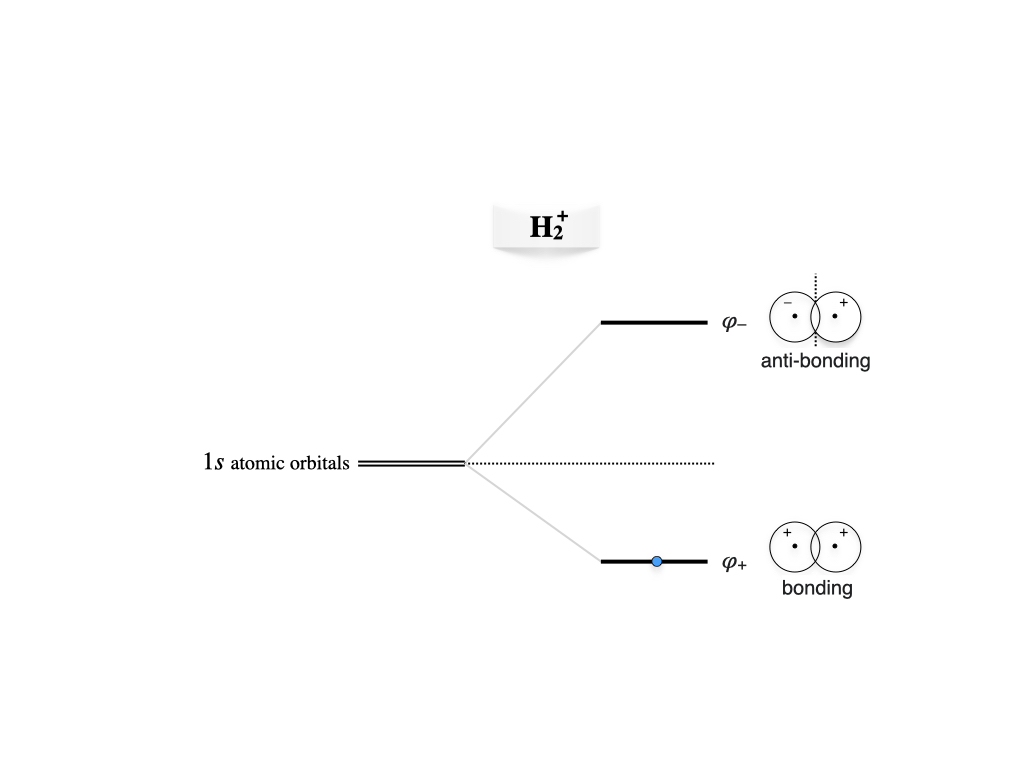
\includegraphics[width=0.7\linewidth]{./img/OEP_figure2} 

}

\caption{Molecular orbitals diagram for the hydrogen molecular cation.}\label{fig:Fig2c12}
\end{figure}

Calculating the values for the integrals and repeating these calculations for different internuclear distances, \(R\), results in the plot of figure \ref{fig:Fig3c12} As we see from the plots, the ground state solution is negative for a vast portion of the plot. The energy is negative because the electronic energy calculated with the bonding orbital is lower than the nuclear repulsion. In other words, the creation of the molecular orbital stabilizes the molecular configuration versus the isolated fragments (one hydrogen atom and one proton).

\begin{figure}

{\centering 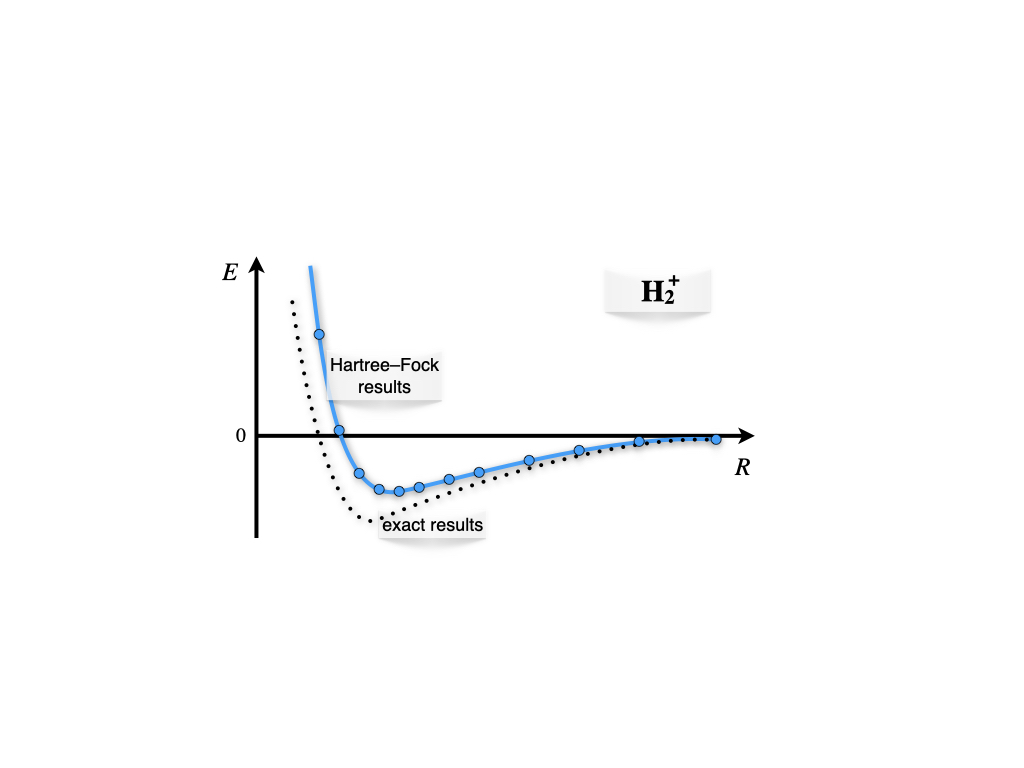
\includegraphics[width=0.7\linewidth]{./img/OEP_figure3} 

}

\caption{Born-Oppenheimer energy landscape for the hydrogen molecular cation.}\label{fig:Fig3c12}
\end{figure}

\hypertarget{the-chemical-bond-in-the-hydrogen-molecule}{%
\section{The Chemical Bond in the Hydrogen Molecule}\label{the-chemical-bond-in-the-hydrogen-molecule}}

\begin{figure}

{\centering 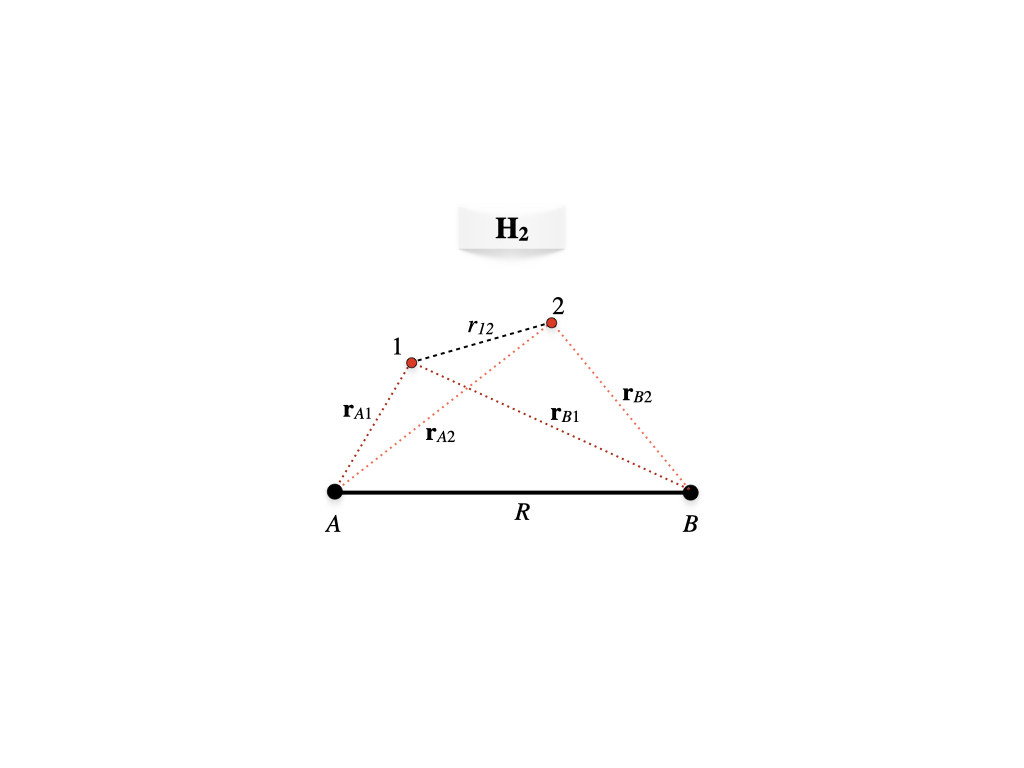
\includegraphics[width=0.7\linewidth]{./img/OEP_figure4} 

}

\caption{Geometry of the hydrogen molecule.}\label{fig:Fig4c12}
\end{figure}

We can now examine the formation of the two-electron chemical bond in the \(\text{H}_2\) molecule. With reference to figure \ref{fig:Fig4c12}, the molecular Hamiltonian for \(\text{H}_2\) in a.u. in the Born-Oppenheimer approximation will be:

\begin{equation}
\begin{aligned}
\hat{H} &= \hat{H}_e+\frac{1}{R} \\
&=\left( -\frac{1}{2}\nabla^2_1-\frac{1}{\mathbf{r}_{A1}}-\frac{1}{\mathbf{r}_{B1}} \right)+\left( -\frac{1}{2}\nabla^2_2-\frac{1}{\mathbf{r}_{A2}}-\frac{1}{\mathbf{r}_{B2}} \right)+\frac{1}{r_{12}}+\frac{1}{R}\\
&= \hat{h}_1+\hat{h}_2+\frac{1}{r_{12}}+\frac{1}{R},
\end{aligned}
\label{eq:bond11}
\end{equation}

where \(\hat{h}\) is the one-electron Hamiltonian. As for the previous case, we can build the first approximation to the molecular wave function by considering two \(1s\) atomic orbitals \(a(\mathbf{r}_1)\) and \(b(\mathbf{r}_2)\) centered at \(A\) and \(B\), respectively, having an overlap \(S\). If we Neglect the electron-electron repulsion term, \(\frac{1}{r_{12}}\), the resulting Hartree-Fock equations are exactly the same as in the previous case. The most important difference, though, is that in this case we need to consider the spin of the two electrons. Proceeding similarly to what we have done for the many-electron atom in chapter \ref{Atoms}, we can build an antisymmetric wave function for \(\text{H}_2\) using a Slater determinant of doubly occupied MOs. For the ground state, we can use the lowest energy orbital obtained from the solution of the Hartree-Fock equations, which we already obtained in eq. \eqref{eq:bond8}. Using a notation that is based on the symmetry of the molecule, this bonding orbital in \(\text{H}_2\) is usually called \(\sigma_g\), where \(\sigma\) refers to the \(\sigma\) bond that forms between the two atoms. The Slater determinant for the ground state is therefore:\footnote{Compare this equation to \eqref{eq:atom6} for the helium atom.}

\begin{equation}
\Psi (\mathbf{x}_{1},\mathbf{x}_{2})= |\sigma_{g}\phi_{\uparrow},\sigma_{g}\phi_{\downarrow}\rangle,=\sigma_{g}(\mathbf{r}_1)\sigma_{g}(\mathbf{r}_2) \frac{1}{\sqrt{2}} \left[ \phi_{\uparrow}\phi_{\downarrow} - \phi_{\downarrow}\phi_{\uparrow} \right],
\label{eq:bond12}
\end{equation}

where:

\begin{equation}
\sigma_{g}=\varphi_{+}=\frac{\left(\psi_{100}\right)_A+\left(\psi_{100}\right)_B}{\sqrt{2+2S}}.
\label{eq:bond13}
\end{equation}

The energies and the resulting MO diagram is similar to that for \(\mathrm{H}_2^+\), with the only difference that two electron will be described by the same \(\sigma_g\) MO (figure \ref{fig:Fig5c12}).

\begin{figure}

{\centering 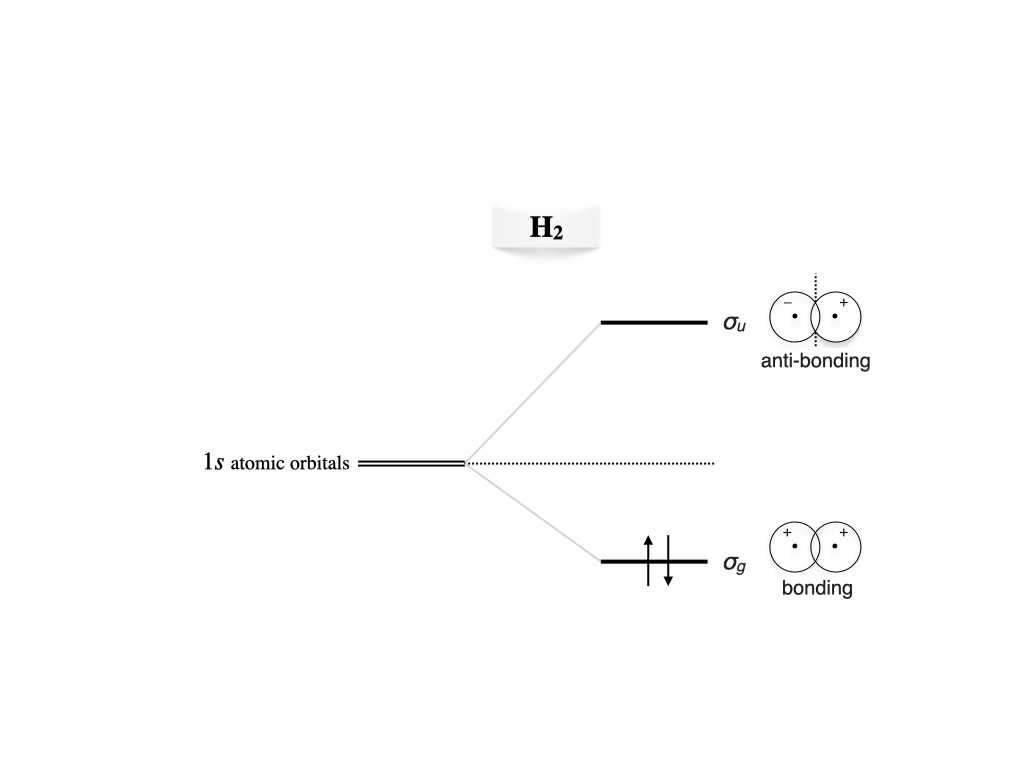
\includegraphics[width=0.7\linewidth]{./img/OEP_figure5} 

}

\caption{Molecular orbitals diagram for the hydrogen molecule.}\label{fig:Fig5c12}
\end{figure}

As for the many-electron atoms, the Hartree-Fock method is just an approximation to the exact solution. The accurate theoretical value for the bond energy at the bond distance of \(R_e=1.4\;a_0\) is \(E= -0.17447\;E_h\). The variational result obtained with the wave function in eq. \eqref{eq:bond12} is \(E= -0.12778\;E_h\), which is \(\sim 73 \%\) of the exact value. The variational coefficient (i.e., the orbital exponent, \(c_0\), that enters the \(1s\) orbital formula \(\psi_{100}=\frac{1}{\pi}\exp[c_0r]\)) is optimized at \(c_0=1.1695\), a value that shows how the orbitals significantly contract due to spherical polarization.

If we scan the Born-Oppenheimer energy landscape using the wave function in eq. \eqref{eq:bond12} as we have done for \(\mathrm{H}_2^+\), we obtain the plot in figure \ref{fig:Fig6c12}.

\begin{figure}

{\centering 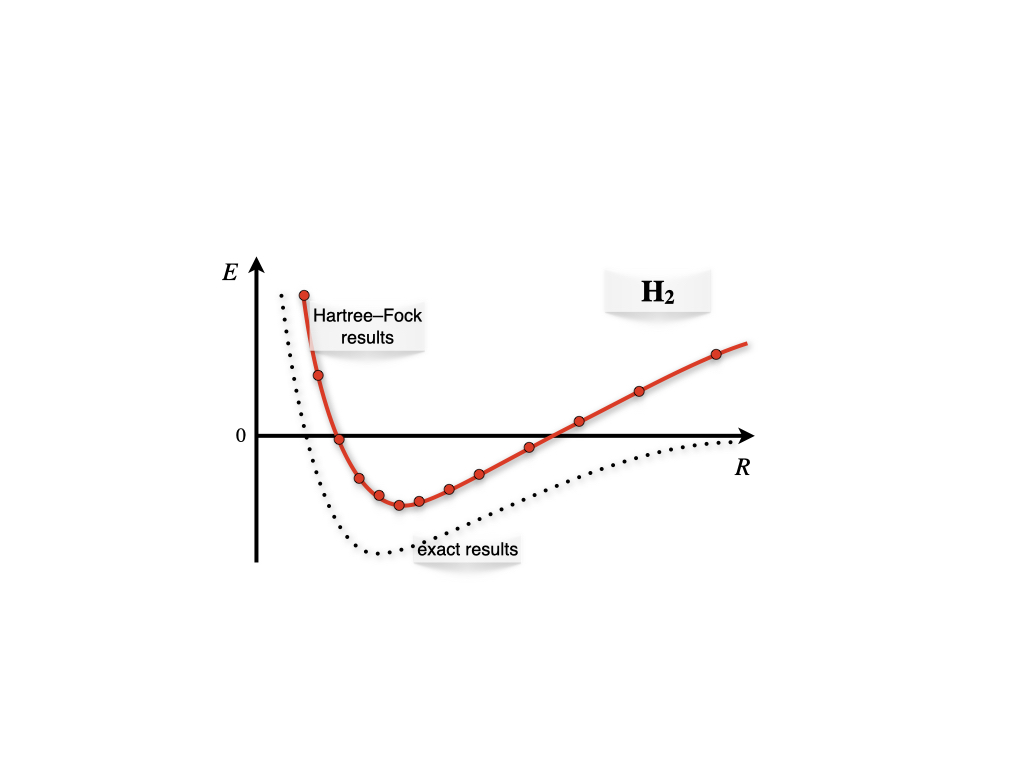
\includegraphics[width=0.7\linewidth]{./img/OEP_figure6} 

}

\caption{Born-Oppenheimer energy landscape for the hydrogen molecule.}\label{fig:Fig6c12}
\end{figure}

As we can see, the Hartree-Fock results for \(\mathrm{H}_2\) describes the formation of the bond qualitatively around the bond distance (minimum of the curve), but they fail to describe the molecule at dissociation. This happens because in eq. \eqref{eq:bond12} both electrons are in the same orbital with opposite spin (electrons are coupled), and the orbital is shared among both centers. At dissociation, this corresponds to an erroneous ionic dissociation state where both electron are localized on either one of the two centers (this center is therefore negatively charged), with the other proton left without electrons. This is in contrast with the correct dissociation, where each electron should be localized around each center (and therefore, it should be uncoupled from the other electron). This error is once again the result of the approximations that are necessary to treat the TISEq of a many-electron system. It is obviously not a failure of quantum mechanics, and it can be easily corrected using more accurate approximations on modern computers.

\hypertarget{Spectroscopy}{%
\chapter{Spectroscopy}\label{Spectroscopy}}

The primary method of measuring the energy levels of a material is through the use of electromagnetic radiation. Experiments involving electromagnetic radiation---matter interaction are called spectroscopies. Since the energy levels of atoms and molecules are discontinuous, they absorb or emit light only at specific energies. These specific values correspond to the energy level difference between the initial and final states and they can be measured as signals in spectroscopic experiments. The intensity of the experimental signals depends on the population of the initial state involved in the transition.

Depending on the type of radiation, as well as the shape of the molecules and the inner details of the instrument that is used, some transition might be visible by the experiment (allowed), while others might not be (forbidden). The analysis of allowed and forbidden transition for each type of spectroscopy results into some mathematical formula that are called \textbf{selection rules}.

To summarize, spectroscopy is mainly the result of the following three effects:

\begin{itemize}
\tightlist
\item
  The energy levels of the atoms or molecules (determining the position of the signals).
\item
  The population of the energy levels (determining the intensity of the signals).
\item
  The selection rules that account for the symmetry and the interaction with the instrument.
\end{itemize}

Spectroscopy is the most important experimental verification of quantum mechanics, since we can use it to validate its theoretical results on the energy levels of atoms and molecules.

\hypertarget{rotational-spectroscopy}{%
\section{Rotational Spectroscopy}\label{rotational-spectroscopy}}

Rotational spectroscopy is concerned with the measurement of the energies of transitions between quantized rotational states of molecules in the gas phase. Rotational transitions of molecules are usually measured in the range \(1-10\; \text{cm}^{-1}\) (microwave radiation) and rotational spectroscopy is therefore usually referred to as \emph{microwave spectroscopy}.

Rotational spectroscopy is actively used by astrophysicists to explore the chemical composition of the interstellar medium using radio telescopes.

The rotational energies are derived theoretically by considering the molecules to be rigid rotors and applying the same treatment that we saw in chapter \ref{Models}. Correction terms might be applied to account for deviation from the ideal rigid rotor case. As we saw in chapter \ref{Models}, the quantized rotational energy levels of a rigid rotor depend on the angular moment of inertia, which in turn depends on the masses of the nuclei and the internuclear distance. Reversing the theoretical procedure of obtaining the energy levels from the distances, we can use the experimental energy levels to derive very precise values of molecular bond lengths (and in some complex case, also of angles). We will discuss below the simplest case of a diatomic molecule. For non-linear molecules, the moments of inertia are multiple, and only a few analytical method of solving the TISEq are available. For the most complicated cases, numerical methods can be used.

\hypertarget{rotation-of-diatomic-molecules}{%
\subsection{Rotation of diatomic molecules}\label{rotation-of-diatomic-molecules}}

Transitions between rotational states can be observed in molecules with a permanent electric dipole moment. The rigid rotor is a good starting point from which to construct a model of a rotating molecule. It is assumed that component atoms are point masses connected by rigid bonds. A linear molecule lies on a single axis and each atom moves on the surface of a sphere around the center of mass. The two degrees of rotational freedom correspond to the spherical coordinates, \(\theta\) and \(\varphi\), which describe the direction of the molecular axis. The quantum state is determined by two quantum numbers \(J\) and \(M\). \(J\) defines the magnitude of the rotational angular momentum, and \(M\) its component about an axis fixed in space, such as an external electric or magnetic field. In the absence of external fields, the energy depends only on \(J\). Under the rigid rotor model, the rotational energy levels, \(F(J)\), of the molecule can be expressed as:

\begin{equation}
F\left(J\right)=BJ\left(J+1\right)\qquad J=0,1,2,\ldots
\label{eq:rot1}
\end{equation}

where \(B\) is the rotational constant of the molecule and is related to its moment of inertia. In a diatomic molecule the moment of inertia about an axis perpendicular to the molecular axis is unique, so:

\begin{equation}
B={\frac{h}{8\pi ^{2}cI_{B}}}={\frac{h}{8\pi ^{2}cI_{C}}},
\label{eq:rot2}
\end{equation}

with:

\begin{equation}
 I=\frac{m_1m_2}{m_1 +m_2}d^2 
 \label{eq:rot3}
\end{equation}

where \(m_1\) and \(m_2\) are the masses of the atoms and \(d\) is the distance between them.

The selection rule for rotational spectroscopy dictate that during emission or absorption the rotational quantum number has to change by unity:

\begin{equation}
 \Delta J = J^{{\prime }} - J^{{\prime \prime }} = \pm 1,
 \label{eq:rot4}
\end{equation}

where \(J^{{\prime }}\) denotes the lower level and \(J^{{\prime \prime }}\) denotes the upper level involved in the transition. Thus, the locations of the lines in a rotational spectrum will be given by

\begin{equation}
{\tilde  \nu }_{{J^{{\prime }}\leftrightarrow J^{{\prime \prime }}}}=F\left(J^{{\prime }}\right)-F\left(J^{{\prime \prime }}\right)=2B\left(J^{{\prime \prime }}+1\right)\qquad J^{{\prime \prime }}=0,1,2,\ldots
\label{eq:rot5}
\end{equation}

The diagram illustrates rotational transitions that obey the \(\Delta J=1\) selection rule is in figure .\footnote{This diagram is taken from \href{https://en.wikipedia.org/wiki/Rotational_spectroscopy\#/media/File:Rotational_spectrum_example.png}{Wikipedia} by user Nnrw, and distributed under CC BY\_SA 3.0 license.} The dashed lines show how these transitions map onto features that can be observed experimentally. Adjacent \(J^{{\prime \prime}}{\leftarrow}J^{{\prime }}\) transitions are separated by \(2B\) in the observed spectrum. Frequency or wavenumber units can also be used for the \(x\) axis of this plot.

\begin{figure}

{\centering 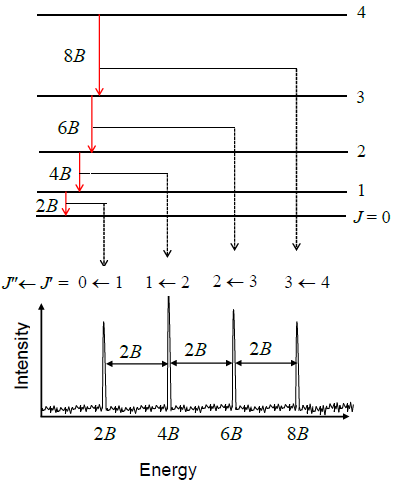
\includegraphics[width=0.5\linewidth]{./img/OEP_wiki5} 

}

\caption{Rotational energy levels and line positions calculated in the rigid rotor approximation.}\label{fig:Fig1c13}
\end{figure}

The probability of a transition taking place is the most important factor influencing the intensity of an observed rotational line. This probability is proportional to the population of the initial state involved in the transition. The population of a rotational state depends on two factors. The number of molecules in an excited state with quantum number \(J\), relative to the number of molecules in the ground state, \(N_J/N_0\) is given by the Boltzmann distribution:

\begin{equation}
\frac{N_J}{N_0}=e^{-\frac{E_J}{kT}} =e^{-\frac {BhcJ(J+1)}{kT}},
\label{eq:rot6}
\end{equation}

where \(k\) is the Boltzmann constant and \(T\) is the absolute temperature. This factor decreases as \(J\) increases. The second factor is the degeneracy of the rotational state, which is equal to \(2J+1\). This factor increases as \(J\) increases. Combining the two factors we obtain:

\begin{equation}
\mathrm{population} \propto (2J+1)e^{-\frac{E_J}{kT}},
\label{eq:rot7}
\end{equation}

in agreement with the experimental shape of rotational spectra of diatomic molecules.

\hypertarget{vibrational-spectroscopy}{%
\section{Vibrational Spectroscopy}\label{vibrational-spectroscopy}}

Vibrational spectroscopy is concerned with the measurement of the energies of transitions between quantized vibrational states of molecules in the gas phase. These transitions usually occur in the middle infrared (IR) region of the electromagnetic wave at approximately \(4,000-400\;\text{cm}^{-1}\) (\(2.5-25\;\mu \text{m}\)). In the gas phase, vibrational transitions are almost always accompanied by changes in rotational energy. Transitions involving changes in both vibrational and rotational states are usually abbreviated as rovibrational transitions. Since changes in rotational energy levels are typically much smaller than changes in vibrational energy levels, changes in rotational state are said to give fine structure to the vibrational spectrum. For a given vibrational transition, the same theoretical treatment that we saw in the previous section for pure rotational spectroscopy gives the rotational quantum numbers, energy levels, and selection rules.

As we have done in the previous section, we will discuss below the simplest case of a diatomic molecule. For non-linear molecules the spectra becomes complicated to calculate, but their interpretation remains an important tool for the analysis of chemical structures.

\hypertarget{vibration-of-heteronuclear-diatomic-molecules}{%
\subsection{Vibration of heteronuclear diatomic molecules}\label{vibration-of-heteronuclear-diatomic-molecules}}

Diatomic molecules with the general formula \(\mathrm{AB}\) have one normal mode of vibration involving stretching of the \(\mathrm{A}-\mathrm{B}\) bond. The vibrational term values, \(G(v)\) can be calculated with the harmonic approximation that we discussed in chapter \ref{Models}. The resulting equidistant energy levels depend on one vibrational quantum number \(v\):

\begin{equation}
G(v) = \omega_e \left( v + \frac{1}{2} \right),
\label{eq:vib1}
\end{equation}

where \(\omega_e\) is the harmonic frequency around equilibrium. When the molecule is in the gas phase, it can rotate about an axis, perpendicular to the molecular axis, passing through the center of mass of the molecule. As we discussed in the previous section, the rotational energy is also quantized, and depend on the rotational quantum number \(J\). The values of the ro-vibrational states are found (in wavenumbers) by combining the expressions for vibration and rotation:

\begin{equation}
G(v)+F_{v}(J)=\left[\omega_e \left(v + \frac{1}{2} \right) +B_{v}J(J+1)\right],
\label{eq:vib2}
\end{equation}

where \(F_{v}(J)\) are the rotational levels at each vibrational state \(v\).\footnote{This is just a first approximation to rovibrational spectroscopy. Corrections for anharmonicity centrifugal distortion are necessary to closely match experimental spectra.}

The selection rule for electric dipole allowed ro-vibrational transitions, in the case of a diamagnetic diatomic molecule is:

\begin{equation} 
\Delta v=\pm 1\ (\pm 2,\pm 3,\ldots),\; \Delta J=\pm 1.
\label{eq:vib3}
\end{equation}

The transition with \(\Delta v =\pm 1\) is known as the \emph{fundamental transition}, while the others are called \emph{overtones}. The selection rule has two consequences:

\begin{enumerate}
\def\labelenumi{\arabic{enumi}.}
\tightlist
\item
  Both the vibrational and rotational quantum numbers must change. The transition \(\Delta v=\pm 1,\;\Delta J=0\) (Q-branch) is forbidden.
\item
  The energy change of rotation can be either subtracted from or added to the energy change of vibration, giving the P- and R- branches of the spectrum, respectively.
\end{enumerate}

\begin{figure}

{\centering 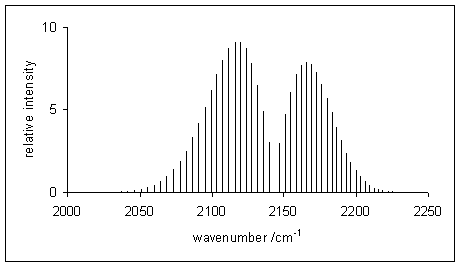
\includegraphics[width=0.5\linewidth]{./img/OEP_wiki6} 

}

\caption{Simulated vibration-rotation line spectrum of carbon monoxide. The P-branch is to the left of the gap at 2140 1/cm, the R-branch on the right.}\label{fig:Fig2c13}
\end{figure}

A typical rovibrational spectrum is reported in figure \ref{fig:Fig2c13} for the \(\mathrm{CO}\) molecule.\footnote{This picture is taken from \href{https://en.wikipedia.org/wiki/Rotational–vibrational_spectroscopy\#/media/File:Vib_rot_CO.png}{Wikipedia} of anonimous user, and distributed under CC BY 3.0 license.} The intensity of the signals is---once again---proportional to the initial population of the levels. Notice how the signals in the spectrum are divided among two sides, the P-branch to the left, and the R-branch to the right. These signals correspond to the transitions reported in figure \ref{fig:Fig3c13}.\footnote{This picture is taken from \href{https://en.wikipedia.org/wiki/Rotational–vibrational_spectroscopy\#/media/File:Vibrationrotationenergy.svg}{Wikipedia} by user David-i98, and under public domain.} Notice how the transitions corresponding to the Q-branch are forbidden by the selection rules, and therefore not observed in the experimental spectrum. The position of the missing Q-branch, however, can be easily obtained from the experimental spectrum as the missing signal between the P- and R- branches. Since the Q-branch transitions do not involve changes in the rotational energy level, their value is directly proportional to \(\omega_e\). This fact makes rovibrational spectroscopy an important experimental tool in the determination of bond distances of diatomic molecules.

\begin{figure}

{\centering 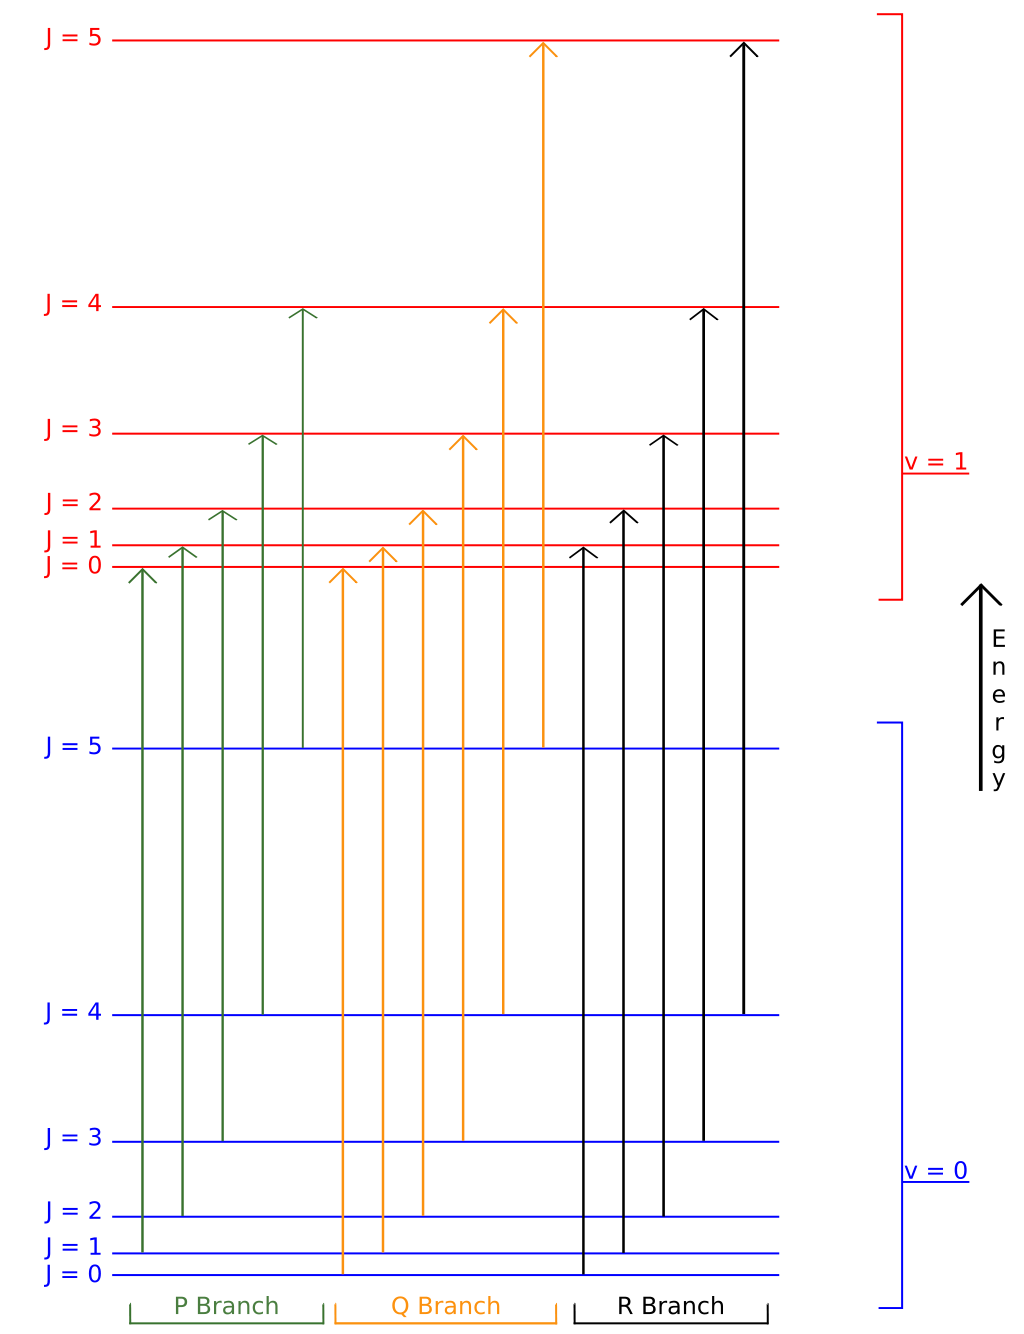
\includegraphics[width=0.5\linewidth]{./img/OEP_wiki7} 

}

\caption{Schematic rovibrational energy level diagram for a linear molecule.}\label{fig:Fig3c13}
\end{figure}

\hypertarget{vibration-of-homonuclear-diatomic-molecules}{%
\subsection{Vibration of homonuclear diatomic molecules}\label{vibration-of-homonuclear-diatomic-molecules}}

The quantum mechanics for homonuclear diatomic molecules is qualitatively the same as for heteronuclear diatomic molecules, but the selection rules governing transitions are different. Since the electric dipole moment of the homonuclear diatomics is zero, the fundamental vibrational transition is electric-dipole-forbidden and the molecules are infrared inactive.

The spectra of these molecules can be observed by a type of IR spectroscopy that is subject to different selection rules. This technique is called \textbf{Raman spectroscopy}, and allows identification of the rovibrational spectra of homonuclear diatomic molecules because their molecular vibration is Raman-allowed.

\hypertarget{electronic-spectroscopy}{%
\section{Electronic Spectroscopy}\label{electronic-spectroscopy}}

Electronic spectroscopy is concerned with the measurement of the energies of transitions between quantized electronic states of molecules. Electronic transitions are always associated with simultaneous changes in vibrational levels. In the gas phase vibronic transitions are also accompanied by changes in rotational energy.

Electronic transitions are typically observed in the visible and ultraviolet regions, in the wavelength range approximately \(200-700\; \text{nm }\) (\(50,000-14,000\; \text{cm}^{-1}\)). When the electronic and vibrational energy changes are drastically different, vibronic coupling (mixing of electronic and vibrational wave functions) can be neglected and the energy of a vibronic level can be taken as the sum of the electronic and vibrational (and rotational) energies; that is, the Born--Oppenheimer approximation applies. The overall molecular energy depends not only on the electronic state but also on the vibrational and rotational quantum numbers, \(v\) and \(J\). In this context, it is conventional to add a double prime \(\left(v^{\prime\prime},J^{\prime\prime}\right)\) for levels of the electronic ground state and a single prime \(\left(v^{\prime},J^{\prime}\right)\) for electronically excited states.

Each electronic transition may show vibrational coarse structure, and for molecules in the gas phase, rotational fine structure. This is true even when the molecule has a zero dipole moment and therefore has no vibration-rotation infrared spectrum or pure rotational microwave spectrum.

It is necessary to distinguish between absorption and emission spectra. With absorption the molecule starts in the ground electronic state, and usually also in the vibrational ground state \(v^{\prime\prime}=0\) because at ordinary temperatures the energy necessary for vibrational excitation is large compared to the average thermal energy. The molecule is excited to another electronic state and to many possible vibrational states \(v^{\prime}=0,1,2,3,ldots\). With emission, the molecule can start in various populated vibrational states, and finishes in the electronic ground state in one of many populated vibrational levels. The emission spectrum is more complicated than the absorption spectrum of the same molecule because there are more changes in vibrational energy level.

As we did for the previous two cases, we will concentrate below on the electronic absorption spectroscopy of diatomic molecules.

\hypertarget{electronic-spectroscopy-of-diatomic-molecules}{%
\subsection{Electronic spectroscopy of diatomic molecules}\label{electronic-spectroscopy-of-diatomic-molecules}}

The vibronic spectra of diatomic molecules in the gas phase also show rotational fine structure. Each line in a vibrational progression will show P- and R- branches. For some electronic transitions there will also be a Q-branch. The transition energies of the lines for a particular vibronic transition are given (in wavenumbers) by:

\begin{equation}
G(J^{\prime },J^{{\prime \prime }})={\bar  \nu }_{{v^{\prime }-v^{{\prime \prime }}}}+B^{\prime }J^{\prime }(J^{\prime }+1)-B^{{\prime \prime }}J^{{\prime \prime }}(J^{{\prime \prime }}+1).
\label{eq:elec1}
\end{equation}

The values of the rotational constants, \(B^{\prime}\) and \(B^{\prime\prime}\) may differ appreciably because the bond length in the electronic excited state may be quite different from the bond length in the ground state. The rotational constant is inversely proportional to the square of the bond length. Usually \(B^{\prime}<B^{\prime\prime}\), as is true when an electron is promoted from a bonding orbital to an antibonding orbital, causing bond lengthening.

The treatment of rotational fine structure of vibronic transitions is similar to the treatment of rotation-vibration transitions and differs principally in the fact that the ground and excited states correspond to two different electronic states as well as to two different vibrational levels. For the P-branch \(J^{\prime }=J^{{\prime \prime}}-1\), so that:

\begin{equation}
\begin{aligned}
{\bar  \nu }_{P}&={\bar  \nu}_{{v^{\prime}-v^{\prime\prime}}}+B^{\prime}(J^{\prime\prime}-1)J^{\prime\prime}-B^{\prime\prime}J^{\prime\prime}(J^{\prime\prime}+1) \\
&={\bar  \nu }_{{v^{\prime}-v^{\prime\prime}}}-(B^{\prime}+B^{\prime\prime})J^{\prime\prime}+(B^{\prime}-B^{\prime\prime}){J^{\prime\prime}}^{2}.
\end{aligned}
\label{eq:elec2}
\end{equation}

Similarly, for the R-branch \(J^{\prime\prime }=J^{{\prime }}-1\), and:

\begin{equation}
\begin{aligned}
{\bar  \nu }_{R} &={\bar  \nu}_{{v^{\prime}-v^{\prime\prime}}}+B^{\prime}J^{\prime}(J^{\prime}+1)-B^{\prime\prime}J^{\prime}(J^{\prime}-1) \\
&={\bar  \nu }_{{v^{\prime}-v^{\prime\prime}}}+(B^{\prime}+B^{\prime\prime})J^{\prime}+(B^{\prime}-B^{\prime\prime}){J^{\prime}}^{2}.
\end{aligned}
\label{eq:elec3}
\end{equation}

Thus, the wavenumbers of transitions in both P- and R- branches are given, to a first approximation, by the single formula:

\begin{equation}
{\bar  \nu }_{{P,R}}={\bar  \nu }_{{v^{\prime },v^{{\prime \prime }}}}+(B^{\prime }+B^{{\prime \prime }})m+(B^{\prime }-B^{{\prime \prime }})m^{2},\quad m=\pm 1,\pm 2\, \ldots.
\label{eq:elec4}
\end{equation}

Here positive \(m\) values refer to the R-branch (with \(m=+J^{\prime}=J^{\prime\prime}+1\)) and negative values refer to the P-branch (with \(m=-J^{\prime\prime}\)).

The intensity of allowed vibronic transitions is governed by the Franck-Condon principle, which states that during an electronic transition, a change from one vibrational energy level to another will be more likely to happen if the two vibrational wave functions overlap more significantly. A diagrammatic representation of electronic spectroscopy and the Frack-Condon principle for a diatomic molecule is presented in figure \ref{fig:Fig4c13}.\footnote{This picture is taken from \href{https://en.wikipedia.org/wiki/Franck–Condon_principle\#/media/File:Franck_Condon_Diagram.svg}{Wikipedia} by user Samoza, and distributed under CC BY-SA 3.0 license.}

\begin{figure}

{\centering 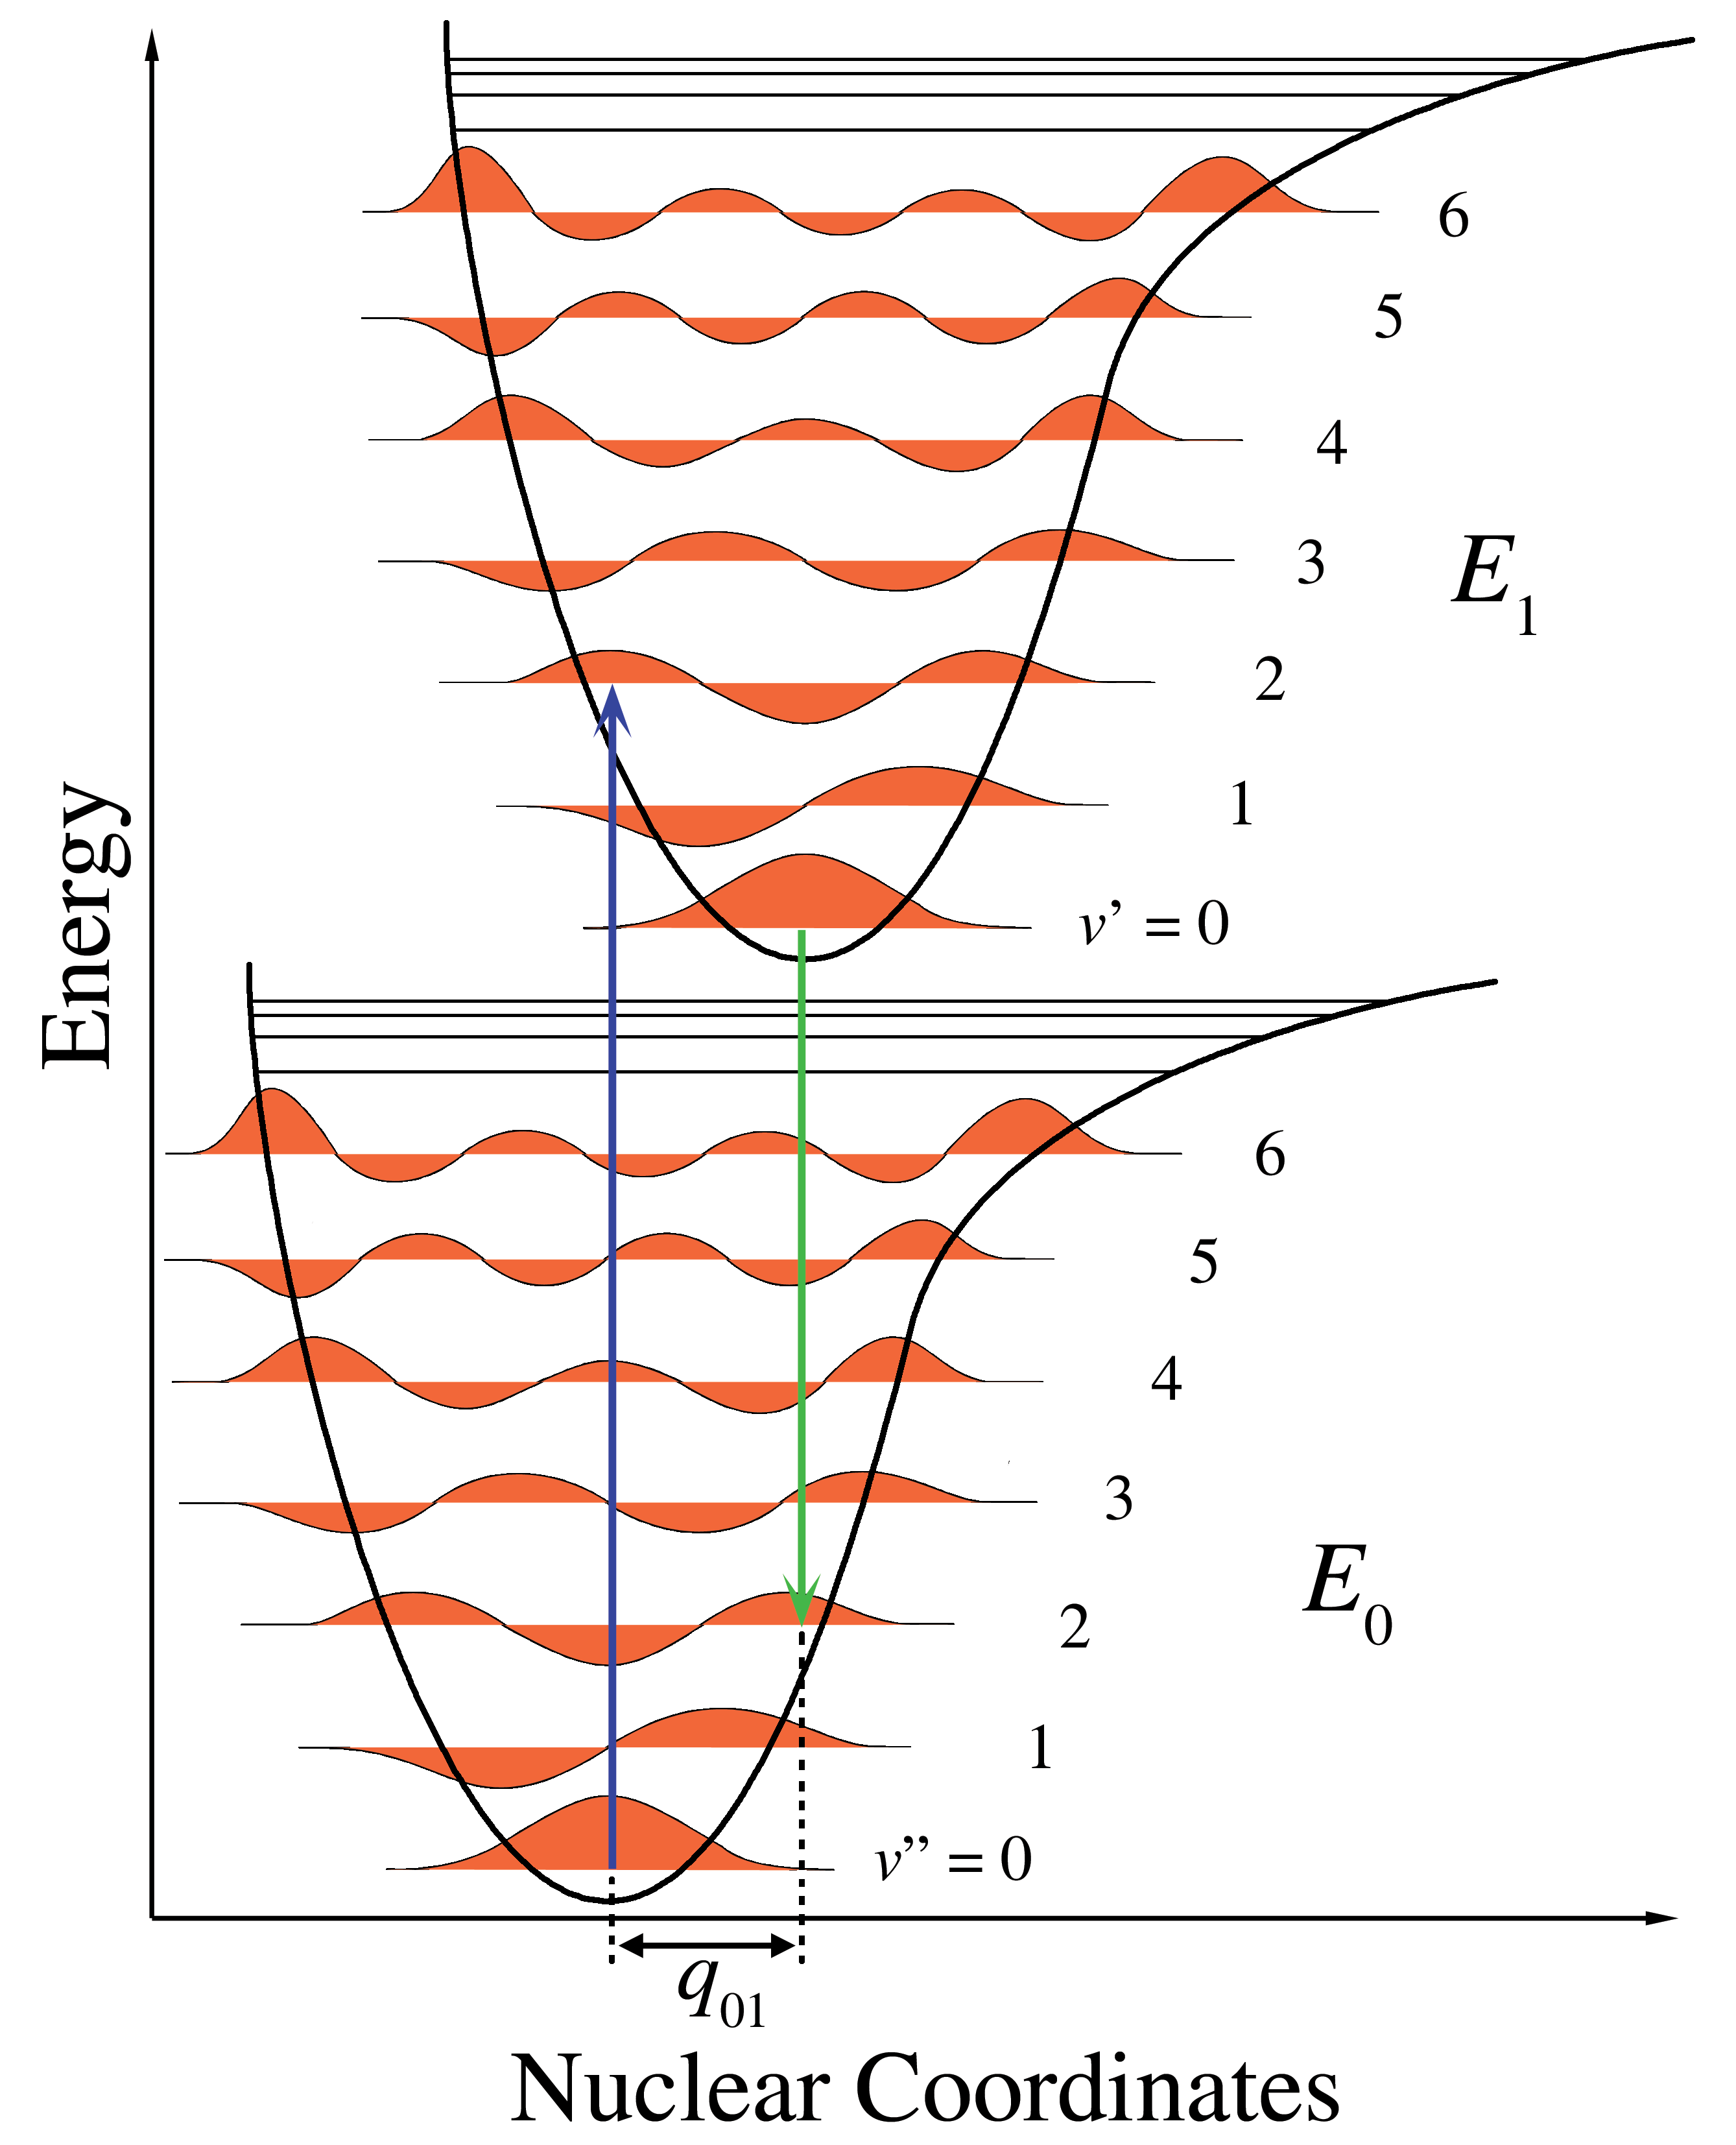
\includegraphics[width=0.7\linewidth]{./img/OEP_wiki8} 

}

\caption{Energy level diagram illustrating the Franck–Condon principle.}\label{fig:Fig4c13}
\end{figure}

\end{document}
